\chapter{Special Functions Defined by Eigenvalue Problems}

\section{Preliminary Discussion of Linear Second Order Differential Equations}
In the present chapter we shall investigate certain classes of functions which have already been defined, Bessel functions, Legendre functions, and general Laplace spherical harmonics. Our point of view will be somewhat more general than in the preceding chapters; we shall permit the independent variable to assume complex values and use the methods of function theory. Furthermore, we shall consider not only the functions mentioned but also the totality of solutions of the corresponding differential equations. We assume it to be known that: linear differential equations of this type, even in the case of a complex independent variable $z=x+iy$, possess two linearly independent solutions, the general solution is a linear combination of these solutions with constant coefficients, and all solutions are regular analytic functions of $z$ except at certain fixed singular points determined by the coefficients. Many important classes of functions can be defined as solutions of such linear differential equations with analytic coefficients.

To obtain solutions of a linear differential equation
\[
L[u]+\mu u=0
\]
in the form of an integral representation, the \emph{method of integral transformation} is often useful; we start with a general outline of this method. In place of the unknown function $u(z)$ we introduce a new unknown function $v(\zeta)$ of the complex variable $\zeta=\xi+i\eta$ by means of equation
\begin{equation}\tag{1}
u(z)=\int_CK(z,\zeta)v(\zeta)\,d\zeta,
\end{equation}
where the transformation kernel $K(z,\zeta)$ (assumed analytic in each of the complex variables) and the path of integration $C$ are to be suitably determined. The differential equation takes the form
\[
\int_C\bigl(L[K]+\mu K\bigr)v(\zeta)\,d\zeta=0;
\]
here the differentiation process $L$ refers to the variable $z$ and it is assumed that the process $L$ is interchangeable with integration.

Now we specify $K$ by subjecting $K(z,\zeta)$ to a partial differential equation
\[
L[K]=A[K]
\]
where $A[K]$ is a linear differential expression containing differentiation only with respect to the variable $\zeta$. Integrating by parts we eliminate these derivatives. The above integral takes the form
\[
\int_CK(z,\zeta)\bigl(B[v]+\mu v\bigr)\,d\zeta;
\]
here $B[v]$ denotes the differential expression adjoint to $A[v]$ (see Ch. V, \S1). In addition to this integral, a term depending on the boundary occurs, which can be made to vanish by a suitable choice of the path of integration. If the partial differential equation for $K$, which can be chosen in various ways, as well as the transformed equation
\[
B[v]+\mu v=0
\]
can be solved explicitly in such a way that the above assumptions hold, then this method leads to the solution $u(z)$ in the indicated integral form.

In analysis such integral transformations occur in various forms. For example the kernel
\[
K(z,\zeta)=e^{z\zeta}\quad\text{or}\quad e^{iz\zeta}
\]
produces the \emph{Laplace transformation}, the kernel
\[
K(z,\zeta)=(z-\zeta)^\alpha
\]
the \emph{Euler transformation} if the path of integration is suitably chosen.

\section{Bessel Functions}
First we shall discuss Bessel's equation
\begin{equation}\tag{2}
z^2u''+zu'+z^2u-\lambda^2u=0
\end{equation}
and all its solutions, considering both $z$ and the parameter $\lambda$ as complex quantities.

\subsection{Application of the Integral Transformation}
We subject equation (2) to the transformation (1). Substitution in the differential equation yields
\[
\int_C\bigl(z^2K_{zz}+zK_z+z^2K-\lambda^2K\bigr)v(\zeta)\,d\zeta=0.
\]
We now require that $K$ satisfy the equation
\[
z^2K_{zz}+zK_z+z^2K+K_{\zeta\zeta}=0,
\]
for which the function
\[
K(z,\zeta)=e^{\pm iz\sin\zeta}
\]
is a single-valued regular solution throughout the $z$- and $\zeta$-planes. Equation (2) becomes
\[
\int_C\bigl(K_{\zeta\zeta}+\lambda^2K\bigr)v(\zeta)\,d\zeta=0
\]
or, integrating by parts,
\[
\int_CK(z,\zeta)\bigl(v''+\lambda^2v\bigr)\,d\zeta
+\int_C\frac{\partial}{\partial\zeta}\{K_\zeta v-Kv'\}\,d\zeta=0.
\]
Since the transformed equation $v''+\lambda^2v=0$ has the solutions $e^{\pm i\lambda\zeta}$, we have only to choose the path of integration in a suitable way. We notice that on the vertical portions of the paths denoted by $L_1$ and $L_2$ in Figures 9 and 10, the real part of $-iz\sin\zeta$ is negative for $\Re(z)>0$ and approaches $-\infty$ exponentially with increasing $|\zeta|$. Therefore, if we set $K(z,\zeta)=e^{-iz\sin\zeta}$, the expression $K_\zeta v-Kv'$ tends to zero in both directions on $L_1$ and $L_2$, and we obtain the integrals

\begin{center}
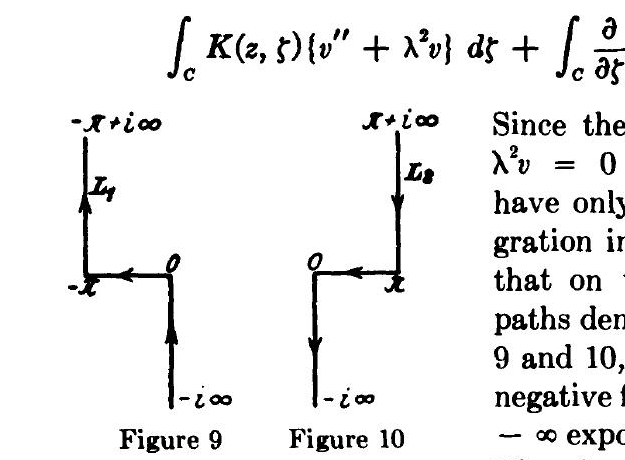
\includegraphics[width=0.44\textwidth]{figures/ch07_fig9_10.png}
\end{center}

\begin{equation}\tag{3}
H_\lambda^1(z)=-\frac1\pi\int_{L_1}e^{-iz\sin\zeta+i\lambda\zeta}\,d\zeta,
\qquad
H_\lambda^2(z)=-\frac1\pi\int_{L_2}e^{-iz\sin\zeta+i\lambda\zeta}\,d\zeta,
\end{equation}
as the two solutions of equation (2), the so-called \emph{Hankel functions}. It can be easily verified that these integrals converge for $\Re(z)>0$ and satisfy the assumptions necessary for their differentiation.

\subsection{Hankel Functions}
The Hankel functions $H_\lambda^1(z)$ and $H_\lambda^2(z)$ are defined by the integrals (3) only in the right half-plane $\Re(z)>0$. However, it is easy to continue them analytically:

If, for fixed $z=x+iy$, we set
\[
f(\zeta)=-iz\sin\zeta+i\lambda\zeta,
\qquad
\zeta=\xi+i\eta,
\qquad
\lambda=a+ib,
\]
then
\[
\Re f(\zeta)=y\sin\xi\cosh\eta+x\cos\xi\sinh\eta-b\xi-a\eta,
\]
\[
\Im f(\zeta)=-x\sin\xi\cosh\eta+y\cos\xi\sinh\eta+a\xi-b\eta.
\]
If, instead of $0$ and $-\pi$, we take the abscissas $\xi_0$ and $-\pi-\xi_0$ for the vertical portions of the path $L_1$, the integral $\int_{L_1'}e^{f(\zeta)}\,d\zeta$ taken over the new path $L_1'$ remains convergent for those $z$ for which
\[
y\sin\xi_0-x\cos\xi_0<0
\]
holds, i.e. for all $z$ in the half-plane bounded by the line
\[
y\sin\xi_0-x\cos\xi_0=0.
\]
Both paths of integration may be used in that part of this half-plane which also lies in the half-plane $x>0$. It is clear from Cauchy's integral theorem that they give the same result. In the remaining part, however, the integral over the new path furnishes the analytic continuation of the function $H_\lambda^1(z)$. If, in an appropriate way, we let $\xi_0$ run through an unbounded sequence of positive and, similarly, through a sequence of negative values, we gradually obtain the complete analytic continuation of the function $H_\lambda^1(z)$; i.e. we obtain a Riemann surface with a branch point at the origin the order of which depends on $\lambda$.

For $\xi_0=-\pi/2$ the horizontal segment of the path of integration vanishes, and for $H_\lambda^1(z)$ we obtain the integral
\[
H_\lambda^1(z)=\frac{e^{-i\lambda\pi/2}}{\pi i}\int_{-\infty}^{\infty}e^{iz\cosh\eta-\lambda\eta}\,d\eta.
\]

% --- printed p.470 ---
which represents the function in the upper half-plane $\Im(z)>0$.
If we permit $z$ to become infinite in the sector
\[
\delta\le \arg z\le \pi-\delta,
\]
the integrand tends to zero over the entire path of integration; hence the function $H_\lambda^1(z)$ also tends to zero since the integral converges uniformly in every subset $\Im(z)\ge \rho>0$. Similarly, we find the function $H_\lambda^2(z)$ tends to zero as $z$ approaches infinity in the sector
\[
-\pi+\delta\le \arg z\le -\delta.
\]
We therefore have the result:

\emph{The Hankel function $H_\lambda^1(z)$ tends to zero when the variable $z$ tends to infinity in a sector $\delta\le \arg z\le \pi-\delta$ of the upper half-plane. The Hankel function $H_\lambda^2(z)$ tends to zero when $z$ tends to infinity in a sector $-\pi+\delta\le \arg z\le -\delta$ of the lower half-plane.}

From the behavior of the Hankel functions at infinity, it follows that:\footnote{This statement is true only for the initial branches of the functions $H_\lambda^1(z)$ and $H_\lambda^2(z)$; the remaining branches are obtained as linear combinations of the original branches, and do not exhibit the described behavior.}
\emph{neither the function $H_\lambda^1(z)$ nor the function $H_\lambda^2(z)$ vanishes identically, and they are linearly independent for every $\lambda$.}

To prove this, we show that, as $|z|$ increases, the functions $H_\lambda^2(z)$ and $H_\lambda^1(z)$ increase without limit on the positive and negative imaginary axes, respectively.

We obtain a representation of $H_\lambda^2(z)$ which converges on the positive imaginary axis by taking the values $-\xi_0$ and $\pi+\xi_0$ for the abscissas of the portions of the path $L_2'$, where $\xi_0$ is any number in the interval $0<\xi_0\le \pi/2$. Since the integrals $\int e^{f(\zeta)}\,d\zeta$ over these portions converge to zero with increasing $y$, we need only investigate the remaining integral
\[
\int_{\pi+\xi_0}^{-\xi_0}e^{y\sin\xi-b\xi+ia\xi}\,d\xi;
\]
substituting $\xi=\xi'+\pi/2$, this integral becomes
\[
\int_0^{(\pi/2)+\xi_0}\cosh b\xi\,e^{y\cos\xi}\cos a\xi\,d\xi.
\]

% --- printed p.471 ---
But this integral increases without limit as $y\to\infty$; this is immediately clear if $|a|\le1$ and can be seen by somewhat more precise estimates\footnote{Let $\xi_0$ be chosen in such a way that $\pi/2+\xi_0$ is an integral multiple of $\pi/2a$. Then the integral in question becomes
\[
\int_0^{n\pi/2a}\cosh b\xi\,e^{y\cos\xi}\cos a\xi\,d\xi
=\frac1a\int_0^{\pi/2}\cos\xi\left\{\sum_{\nu=0}^{n-1}(-1)^\nu\cosh\frac ba\left(\xi+\nu\frac\pi2\right)e^{y\cos\frac1a\left(\xi+\nu\frac\pi2\right)}\right\}\,d\xi.
\]
Here the first term of the sum dominates as $y$ increases, since the exponent $\cos(\xi/a)$ is larger by at least the amount $1-\cos(\pi/2a)$ than any of the following exponents $\cos\frac1a(\xi+\nu\pi/2)$; this term increases with $y$ beyond all bounds.} if $|a|>1$.

The discussion is analogous for the function $H_\lambda^1(z)$ and the negative imaginary axis.

The linear independence of the functions $H_\lambda^1(z)$ and $H_\lambda^2(z)$ implies that the Hankel functions yield the totality of solutions of Bessel's equation. For, every solution may be represented as a linear combination
\[
c_1H_\lambda^1(z)+c_2H_\lambda^2(z).
\]
We observe, in addition, that \emph{the Hankel functions $H_\lambda^1(z)$ and $H_\lambda^2(z)$ are determined uniquely, up to a factor not containing $z$, by their behavior at infinity and by equation (2).} For, if there were two linearly independent solutions of Bessel's equation having the described property, say for the upper half-plane, then every solution---and, in particular, $H_\lambda^2(z)$---would have to have this property. But this contradicts the fact just proved that $|H_\lambda^2(z)|$ increases without limit on the positive imaginary axis.

Finally, we consider the Hankel functions, for fixed $z\ne0$, with respect to their \emph{dependence on the parameter $\lambda$}. Since the integrand in (3) depends analytically on $\lambda$ and the integrals converge uniformly in every finite $\lambda$-domain, it follows that \emph{the Hankel functions are analytic functions of $\lambda$}; in fact, \emph{they are integral transcendental functions.}

\subsection{Bessel and Neumann Functions}
The solutions of equation (2) which are real for real $\lambda$ and $z$ are of particular interest in physics. In order to find expressions for them, we write
\begin{equation}\tag{4}
H_\lambda^1(z)=J_\lambda(z)+iN_\lambda(z),\qquad
H_\lambda^2(z)=J_\lambda(z)-iN_\lambda(z),
\end{equation}

% --- printed p.472 ---
where
\begin{equation}\tag{5}
J_\lambda(z)=\frac12\bigl(H_\lambda^1(z)+H_\lambda^2(z)\bigr)
\end{equation}
is called the \emph{Bessel function} of index $\lambda$ and
\begin{equation}\tag{5'}
N_\lambda(z)=\frac1{2i}\bigl(H_\lambda^1(z)-H_\lambda^2(z)\bigr)
\end{equation}
the corresponding \emph{Neumann function}. Since the determinant
\[
\begin{vmatrix}
\frac12&\frac12\\[2pt]
\frac1{2i}&-\frac1{2i}
\end{vmatrix}=\frac i2
\]
of the substitution is different from zero, \emph{the functions $J_\lambda(z)$ and $N_\lambda(z)$ are linearly independent for all $\lambda$.}

For real $z$ and real $\lambda$ the Hankel functions $H_\lambda^1(z)$ and $H_\lambda^2(z)$ are complex conjugates of each other. For, if we replace $\zeta$ by $-\bar\zeta$ in the representation
\[
\overline{H_\lambda^1(z)}=-\frac1\pi\int_{\bar L_1}e^{iz\sin\bar\zeta-i\lambda\bar\zeta}\,d\bar\zeta,
\]
where $\bar L_1$ is the reflection of $L_1$ across the real axis, we have
\[
\overline{H_\lambda^1(z)}=\frac1\pi\int_{-\bar L_1}e^{-iz\sin\zeta+i\lambda\zeta}\,d\zeta;
\]
since the path $-\bar L_1$ is the same as $L_2$ taken in the negative sense, we obtain
\[
\overline{H_\lambda^1(z)}=-\frac1\pi\int_{L_2}e^{-iz\sin\zeta+i\lambda\zeta}\,d\zeta=H_\lambda^2(z).
\]
Hence, $J_\lambda(z)$ is the real and $N_\lambda(z)$ the imaginary part of the Hankel function $H_\lambda^1(z)$ for real $\lambda$ and $z$, and therefore $J_\lambda(z)$ and $N_\lambda(z)$ are real.

The function $H_{-\lambda}^\nu(z)$ ($\nu=1,2$) is a solution of Bessel's equation for every value of $\lambda$ for which $H_\lambda^\nu(z)$ is a solution, since only $\lambda^2$ appears in the differential equation. The functions $H_\lambda^\nu(z)$ and $H_{-\lambda}^\nu(z)$ cannot be linearly independent because, by subsection 2, they show the same behavior at infinity.

% --- printed p.473 ---
In fact, if we introduce the new variable of integration $-\zeta-\pi$ in the representation
\[
H_{-\lambda}^1(z)=-\frac1\pi\int_{L_1}e^{-iz\sin\zeta-i\lambda\zeta}\,d\zeta,
\]
we at once obtain the relation
\begin{equation}\tag{6}
H_{-\lambda}^1(z)=e^{i\lambda\pi}H_\lambda^1(z)
\end{equation}
and, by means of a similar calculation,
\begin{equation}\tag{6'}
H_{-\lambda}^2(z)=e^{-i\lambda\pi}H_\lambda^2(z).
\end{equation}
For the Bessel and Neumann functions of negative index one obtains
\begin{equation}\tag{7}
J_{-\lambda}(z)=\frac{e^{i\lambda\pi}H_\lambda^1(z)+e^{-i\lambda\pi}H_\lambda^2(z)}{2}
\end{equation}
and
\begin{equation}\tag{7'}
N_{-\lambda}(z)=\frac{e^{i\lambda\pi}H_\lambda^1(z)-e^{-i\lambda\pi}H_\lambda^2(z)}{2i};
\end{equation}
unlike the Hankel functions, they are not linearly dependent on the functions $J_\lambda(z)$ and $N_\lambda(z)$, respectively, for every $\lambda$, but only for those values of $\lambda$ for which the determinant
\[
\frac14\begin{vmatrix}
e^{i\lambda\pi}&e^{-i\lambda\pi}\\
1&1
\end{vmatrix}=\frac i2\sin\lambda\pi
\]
vanishes, in other words, only when $\lambda$ is an integer $n$. In this case we have
\begin{equation}\tag{8}
J_{-n}(z)=(-1)^nJ_n(z)
\end{equation}
and
\begin{equation}\tag{8'}
N_{-n}(z)=(-1)^nN_n(z).
\end{equation}
The \emph{general solution} of equation (2) can therefore be represented in the form
\[
c_1J_\lambda(z)+c_2J_{-\lambda}(z)
\]

% --- printed p.474 ---
when $\lambda$ is not an integer $n$. On the other hand, if $\lambda=n$ we use the sum
\[
c_1J_n(z)+c_2N_n(z).
\]
It will be seen later, however, that even in this case $N_n(z)$ can be calculated easily from $J_n(z)$ and $J_{-n}(z)$ (see subsection 9).

\subsection{Integral Representations of Bessel Functions}
If we add the integrals (3) for $H_\lambda^1(z)$ and $H_\lambda^2(z)$, the paths of integration over the negative imaginary axis cancel and in the right half-plane $\Re(z)>0$ we obtain the representation
\begin{equation}\tag{9}
J_\lambda(z)=-\frac1{2\pi}\int_L e^{-iz\sin\zeta+i\lambda\zeta}\,d\zeta
\end{equation}
for $J_\lambda(z)$, where $L$ is the path indicated in Figure 11.

\begin{center}
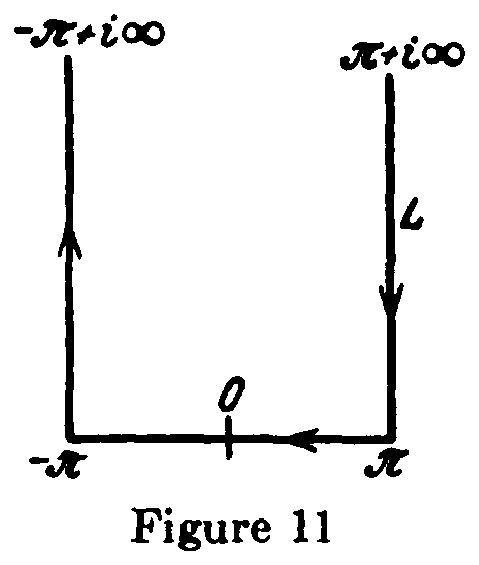
\includegraphics[width=0.29\textwidth]{figures/ch07_fig11.png}
\end{center}

In particular, if $\lambda=n$ is an integer the integrals over the vertical portions of the path $L$ also cancel, because of the periodicity of the integrand. It follows that
\begin{equation}\tag{10}
J_n(z)=\frac1{2\pi}\int_{-\pi}^{\pi}e^{iz\sin\zeta-in\zeta}\,d\zeta
\end{equation}
or, since the real part of the integrand is an even function and the imaginary part is odd,
\begin{equation}\tag{10'}
J_n(z)=\frac1\pi\int_0^\pi\cos(z\sin\zeta-n\zeta)\,d\zeta.
\end{equation}
By means of these integrals $J_n(z)$ is defined for all $z$. We see that \emph{the Bessel functions with integral index are regular and single-valued in the whole plane and hence are integral functions.}

The representation (10) implies also that $J_n(z)$ is the $n$-th Fourier coefficient in the Fourier expansion of
\begin{equation}\tag{11}
e^{iz\sin\zeta}=\sum_{-\infty}^{\infty}J_n(z)e^{in\zeta}
\end{equation}
with respect to $\zeta$. This expansion can be considered as the definition of the function $J_n(z)$ for integral $n$ by means of a \emph{generating function} $e^{iz\sin\zeta}$.

% --- printed p.475 ---
For real $z$ and $\zeta$, (11) yields the relations
\[
\cos(z\sin\zeta)=\sum_{-\infty}^{\infty}J_n(z)\cos n\zeta,
\]
\[
\sin(z\sin\zeta)=\sum_{-\infty}^{\infty}J_n(z)\sin n\zeta,
\]
which also hold for complex $z$ and $\zeta$.
If we observe that
\[
J_{-n}(z)=(-1)^nJ_n(z)
\]
we obtain
\begin{equation}\tag{12}
\begin{aligned}
\cos(z\sin\zeta)&=J_0(z)+2\sum_{1}^{\infty}J_{2n}(z)\cos2n\zeta,\\
\sin(z\sin\zeta)&=2\sum_{1}^{\infty}J_{2n-1}(z)\sin(2n-1)\zeta;
\end{aligned}
\end{equation}
in particular for $\zeta=\pi/2$ we have
\[
\cos z=J_0(z)-2J_2(z)+2J_4(z)-+\cdots,
\]
\[
\sin z=2J_1(z)-2J_3(z)+ -\cdots.
\]
If the new variable of integration $\zeta'=e^{-i\zeta}$ is introduced in (9), it follows that
\begin{equation}\tag{13}
J_\lambda(z)=\frac1{2\pi i}\int_L e^{z(\zeta-\zeta^{-1})/2}\zeta^{-\lambda-1}\,d\zeta,
\end{equation}
where $L$ is the path shown in Figure 12. It extends on both sides of the negative real axis up to the point $\zeta=-1$ and then circles the origin along the unit circle.\footnote{We could have obtained this representation directly, on the basis of the method outlined in \S1, by requiring the transformation kernel to satisfy the differential equation
\[
z^2K_{zz}+zK_z+z^2K-\zeta(\zeta K_\zeta)_\zeta=0,
\]
which is solved by the function $K=e^{z(\zeta-\zeta^{-1})/2}$. The transformed differential equation is then $[\zeta(\zeta v)']'-\lambda^2v=0$; it has the solution $v=\zeta^{\pm\lambda-1}$.}

\begin{center}
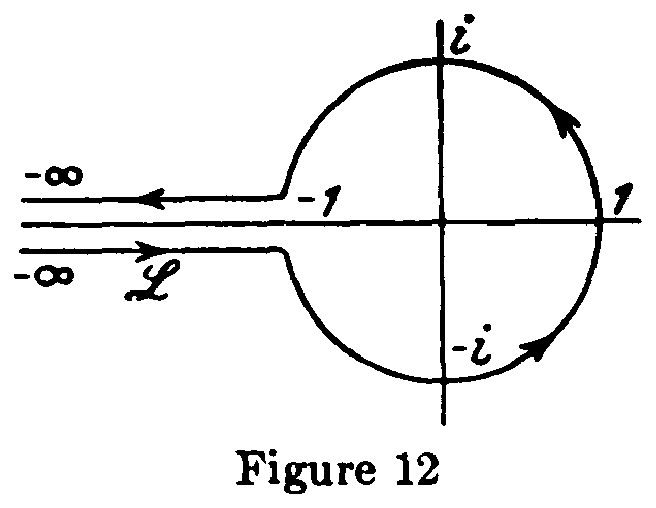
\includegraphics[width=0.31\textwidth]{figures/ch07_fig12.png}
\end{center}

% --- printed p.476 ---
For integral $\lambda=n$ the integrals on the straight portions cancel, and we have
\begin{equation}\tag{14}
J_n(z)=\frac1{2\pi i}\oint e^{z(\zeta-\zeta^{-1})/2}\zeta^{-n-1}\,d\zeta.
\end{equation}
Thus $J_n(z)$ is the $n$-th coefficient in the Laurent expansion
\begin{equation}\tag{15}
e^{z(\zeta-\zeta^{-1})/2}=\sum_{-\infty}^{\infty}J_n(z)\zeta^n.
\end{equation}
This expansion could also have been employed in the definition of $J_n(z)$ for integral $n$.

If we make the transformation $\zeta=2v/z$ in (13)---at first under the assumption of real $z>0$---taking the same path of integration we find
\begin{equation}\tag{16}
J_\lambda(z)=\frac1{2\pi i}\left(\frac z2\right)^\lambda\int_L e^{v-z^2/4v}v^{-(\lambda+1)}\,dv.
\end{equation}
But since the integral on the right converges for all values of $z$, (16) furnishes a representation of the Bessel functions for all $z$. In particular, we see that \emph{the quotient $J_\lambda(z)/z^\lambda$ is an integral function of $z$ for every $\lambda$.}

\subsection{Another Integral Representation of the Hankel and Bessel Functions}
Another integral representation for the Bessel functions is obtained by considering the differential equation for $J_\lambda(z)/z^\lambda$ and applying the Laplace transformation. (Indeed, it seems reasonable to expect that in this way we shall arrive at particularly simple results, since $J_\lambda(z)/z^\lambda$ is a single-valued function of $z$.) For this purpose, we introduce in the equation
\[
u''+\frac1zu'+\left(1-\frac{\lambda^2}{z^2}\right)u=0
\]
the new variable $\omega(z)$ by means of
\[
u=\omega z^\lambda,
\]
from which we obtain
\begin{equation}\tag{17}
z\omega''+(2\lambda+1)\omega'+z\omega=0.
\end{equation}
Writing
\[
\omega(z)=\int_CK(z,\zeta)v(\zeta)\,d\zeta,\qquad K=e^{z\zeta},
\]

% --- printed p.477 ---
we obtain
\[
\int_C\{zK_{zz}+(2\lambda+1)K_z+zK\}v(\zeta)\,d\zeta=0.
\]
In the special case of the Laplace transformation we have
\[
K_z=\zeta K,
\qquad
K_\zeta=zK,
\]
and hence $zK_{zz}=\zeta^2K_\zeta$; we therefore obtain
\[
\int_C\{(1+\zeta^2)K_\zeta+(2\lambda+1)\zeta K\}v(\zeta)\,d\zeta
\]
\[
=-\int_C K(z,\zeta)\{(1+\zeta^2)v'-(2\lambda-1)\zeta v\}\,d\zeta
+\int_C\frac{\partial}{\partial\zeta}\bigl(Kv(1+\zeta^2)\bigr)\,d\zeta=0.
\]
Thus the differential equation is solved if $v(\zeta)$ and $C$ are determined in such a way that
\[
(1+\zeta^2)v'(\zeta)-(2\lambda-1)\zeta v(\zeta)=0
\]
and $e^{z\zeta}v(\zeta)(1+\zeta^2)$ takes equal values at the ends of $C$. From
\[
\frac{v'(\zeta)}{v(\zeta)}=\frac{2\lambda-1}{1+\zeta^2}\,\zeta
\]
we have
\[
v(\zeta)=c(1+\zeta^2)^{\lambda-1/2}.
\]
Thus
\[
\omega(z)=c\int_C e^{z\zeta}(1+\zeta^2)^{\lambda-1/2}\,d\zeta
\]
or, if we introduce $i\zeta$ as a new variable of integration, include $i(-1)^{\lambda-1/2}$ among the constants, and denote the path of integration by $C$, we have
\[
\omega(z)=c\int_C e^{iz\zeta}(\zeta^2-1)^{\lambda-1/2}\,d\zeta.
\]
In order to find an admissible path of integration, we first construct the Riemann surface of the integrand which is one-valued on the

% --- printed p.478 ---
Riemann surface of $\log(\zeta-1)+\log(\zeta+1)=\chi$. If we cut the $\zeta$-plane along two rays parallel to the positive imaginary axis, starting at $\zeta=+1$ and $\zeta=-1$ and ending at $\zeta=+i\infty$, we obtain a simply connected domain in which a branch of $\chi$ is uniquely determined by the value of the imaginary part of $\chi$ on the positive real axis of the $\zeta$-plane. We define two branches $B_1$ and $B_2$ of $\chi$ such that the imaginary part of $\chi$ is zero on $B_1$ and equals $2\pi i$ on $B_2$ for real positive values of $\zeta$. A path crossing either of the branch cuts from the right-hand side to the left-hand side leads from $B_1$ into $B_2$.

\begin{center}
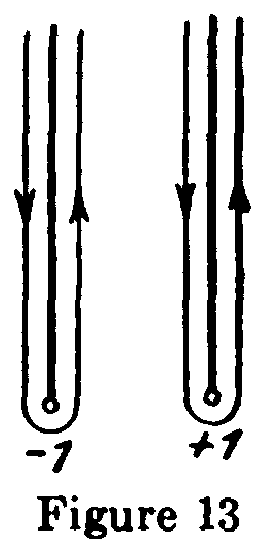
\includegraphics[width=0.16\textwidth]{figures/ch07_fig13.png}
\end{center}

Now let $C_1$ and $C_2$ denote paths lying in the branches $B_1$ and $B_2$, respectively, such that $C_1$ encloses the ray starting from $\zeta=+1$ and $C_2$ encloses the ray starting from $\zeta=-1$ without intersecting either of these rays (see Figure 13). Instead of introducing rays through $\zeta=\pm1$ which are parallel to the imaginary axis, we can introduce rays making an angle $\alpha$ with the positive real axis (where $0<\alpha<2\pi$) and then define $C_1$ and $C_2$ as before.

The integral $\omega(z)$ converges on $C_1$ or $C_2$ for those $z$ for which $\Re(iz\zeta)$ tends to $-\infty$ along the ray. At the same time the expression
\[
Kv(\zeta^2-1)=(\zeta^2-1)^{\lambda+1/2}e^{iz\zeta}
\]
tends to zero at both ends of the path of integration; in other words, $\omega(z)$ is a solution of (17). If the ray makes the angle $\alpha$ with the $\xi$-axis, this will be the case when
\[
y\cos\alpha+x\sin\alpha>0
\]
and thus when $z=x+iy$ lies in one of the half-planes bounded by the line $y\cos\alpha+x\sin\alpha=0$. However, we can continue the integrals analytically, as in subsection 2, by letting $\alpha$ run through an unbounded sequence of positive values and a similar sequence of negative values in a suitable way. In particular, if for both paths we choose $\alpha=\pi/2$ as in Figure 13, both integrals converge in the right half-plane $\Re(z)>0$. If we rotate the path $C_1$ so that it lies along the positive real axis, then the corresponding integral converges in the upper half-plane and tends to zero as $z$ increases without limit in the sector
\[
\delta\le \arg z\le\pi-\delta\qquad(0<\delta<\pi/2).
\]

% --- printed p.479 ---
According to the observation of subsection 2, the integral must therefore coincide, up to a factor independent of $z$, with $H_\lambda^1(z)/z^\lambda$. We find
\[
H_\lambda^1(z)=a_1z^\lambda\int_{C_1}e^{iz\zeta}(\zeta^2-1)^{\lambda-1/2}\,d\zeta
\]
and similarly
\[
H_\lambda^2(z)=a_2z^\lambda\int_{C_2}e^{iz\zeta}(\zeta^2-1)^{\lambda-1/2}\,d\zeta.
\]
The coefficients $a_1$ and $a_2$, which can depend only on $\lambda$, are equal but have opposite signs. This follows---at first for real $\lambda$---from the remark that the Hankel functions are complex conjugates of each other for real $\lambda$ and $z$ (see subsection 3).

We find\footnote{In order to insure convergence on the positive real axis, we take $C_1$ and $C_2$ parallel to the imaginary axis (see Figure 13).} for real values of $\lambda$ and $z$:
\[
\overline{H_\lambda^{(2)}(z)}=\bar a_2z^\lambda\int_{C_1}e^{iz\zeta}(\zeta^2-1)^{\lambda-1/2}\,d\zeta.
\]
This can be verified by observing that for large values of $|\zeta|$ in the proper branches of $B_1$ and $B_2$, the imaginary part of $\log(\zeta^2-1)$ on the four parallels to the imaginary axis in Figure 13 is approximately (i.e. for $|\zeta|\to\infty$ and for $\zeta$ approaching the branch cuts from different sides), from left to right, $-\pi i$, $\pi i$, $-\pi i$, $\pi i$. Therefore we have
\[
\overline{H_\lambda^{(2)}(z)}=\frac{\bar a_2}{a_1}H_\lambda^{(1)}(z)=H_\lambda^{(1)},
\]
that is $\bar a_2=a_1$. Now we shall show that $a_2=-a_1$ by proving that $a_1$ and $a_2$ are pure imaginary if $\lambda$ is real and $\lambda>-\tfrac12$. Since $a_1$ and $a_2$ depend analytically on $\lambda$, $a_1+a_2=0$ for all values of $\lambda$.

That $a_1$ is pure imaginary can be seen by taking $z=iy$, $y>0$ and by turning the path $C_1$ into a path along the positive real axis from $\zeta=1$ to $\zeta=+\infty$. Then
\[
H_\lambda^{(1)}(iy)=a_1\bigl(1-e^{-2\pi i(\lambda-1/2)}\bigr)(iy)^\lambda
\int_1^\infty e^{-y\zeta}(\zeta^2-1)^{\lambda-1/2}\,d\zeta.
\]
From the formula
\[
H_\lambda^1(iy)=\frac{e^{-\pi i\lambda/2}}{\pi i}\int_{-\infty}^{\infty}e^{-y\cosh\eta-\lambda\eta}\,d\eta
\]

% --- printed p.480 ---
we find that
\[
a_1(\lambda)\cos\pi\lambda=\frac{b(\lambda)}{\pi i}
\]
where $b(\lambda)$ is real and positive for real $\lambda>-\tfrac12$. For such $\lambda$ we have, therefore, $\bar a_1=-a_1$, so that $a_2=-a_1$.

Now since by subsection 2 the Hankel functions and, as we see immediately, also the integrals $\int e^{iz\zeta}(\zeta^2-1)^{\lambda-1/2}\,d\zeta$ depend analytically on $\lambda$, the coefficients $a_1(\lambda)$ and $a_2(\lambda)$ are analytic functions of $\lambda$. In other words, the relation $a_1=-a_2=c$ holds generally.

If we add the two integral representations for the Hankel functions, we can deform the resulting path of integration into the figure eight $\mathfrak A$ of Figure 14, which circles $+1$ in the positive sense and $-1$ in the negative sense. We obtain a representation of the Bessel functions
\[
J_\lambda(z)=cz^\lambda\int_{\mathfrak A}e^{iz\zeta}(\zeta^2-1)^{\lambda-1/2}\,d\zeta,
\]
which, for $\lambda\ne n+\tfrac12$ ($n=0,\pm1,\cdots$), is valid in the entire $z$-plane, since the path of integration lies in the finite part of the plane.

\begin{center}
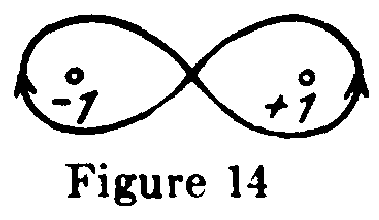
\includegraphics[width=0.23\textwidth]{figures/ch07_fig14.png}
\end{center}

To determine the constant $c$, we compare this representation with the integral representation (16) and find for $z=0$ the relation
\[
\int_{\mathfrak A}(\zeta^2-1)^{\lambda-1/2}\,d\zeta
=\frac1{2^\lambda}\frac1{2\pi i}\int_L e^v v^{-\lambda-1}\,dv.
\]
As will be seen in the next subsection, the integral on the left has the value
\[
\int_{\mathfrak A}(\zeta^2-1)^{\lambda-1/2}\,d\zeta
=2\pi i\frac{\Gamma(\tfrac12)}{\Gamma(\lambda+1)\Gamma(\tfrac12-\lambda)}.
\]
In order to evaluate the integral on the right, we consider the integral
\[
\frac1{2\pi i}\int_L e^v v^{t-1}\,dv,
\]
in particular for positive real values of $t$. Since this integral represents an analytic function of $t$, it is sufficient to reduce it to known analytic functions for such $t$.

% --- printed p.481 ---
Under the assumption $t>0$ we can contract the unit circle to the origin; since the exponent $t-1$ is greater than $-1$, the integral is convergent up to the origin. By Cauchy's theorem, the value of the integral does not change if, instead of integrating over $L$, we integrate from $-\infty$ to $0$ below the real axis and then integrate from $0$ to $-\infty$ above the real axis (see Figure 15):
\[
\frac1{2\pi i}\int_L e^v v^{t-1}\,dv
=\frac1{2\pi i}\int_{-\infty}^{0}e^v v^{t-1}\,dv
+\frac1{2\pi i}\int_0^{-\infty}e^v v^{t-1}\,dv\qquad(t>0),
\]
where the first integral is taken below and the second above the real axis.

\begin{center}
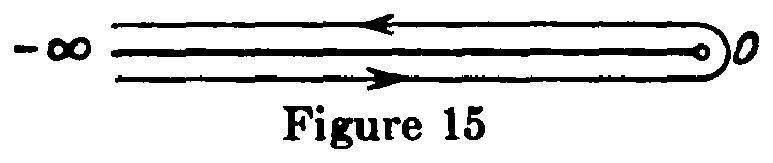
\includegraphics[width=0.37\textwidth]{figures/ch07_fig15.png}
\end{center}

If we set $v=-w$, the first integral becomes
\[
\frac1{2\pi i}\int_\infty^0 w^{t-1}e^{-(t-1)\pi i}e^{-w}(-dw)
=\frac1{2\pi i}\int_0^\infty w^{t-1}e^{-(t-1)\pi i}e^{-w}\,dw,
\]
the second becomes
\[
\frac1{2\pi i}\int_0^\infty w^{t-1}e^{(t-1)\pi i}e^{-w}(-dw);
\]
thus their sum is
\[
\frac1{2\pi i}\int_0^\infty w^{t-1}e^{-w}\bigl(e^{t\pi i}-e^{-t\pi i}\bigr)\,dw.
\]
Since $e^{t\pi i}-e^{-t\pi i}=2i\sin\pi t$ and, by definition,
\[
\int_0^\infty w^{t-1}e^{-w}\,dw=\Gamma(t),
\]
the sum of the integrals has the value
\[
\frac{\sin\pi t}{\pi}\Gamma(t).
\]
From the supplementary theorem for the gamma function,
\[
\Gamma(t)\Gamma(1-t)=\frac\pi{\sin\pi t},
\]
it follows that
\[
\frac{\sin\pi t}{\pi}\Gamma(t)=\frac1{\Gamma(1-t)}.
\]

% --- printed p.482 ---
We have, therefore,
\[
\frac1{2\pi i}\int_L v^{t-1}e^v\,dv=\frac1{\Gamma(1-t)}.
\]
Hence for the constant $c$ we find the value
\[
c=\frac1{2\pi i}\frac1{2^\lambda}\frac{\Gamma(\tfrac12-\lambda)}{\Gamma(\tfrac12)}
\]
and finally obtain for $J_\lambda(z)$ the representation
\begin{equation}\tag{18}
J_\lambda(z)=\frac{\Gamma(\tfrac12-\lambda)}{2\pi i\Gamma(\tfrac12)}
\left(\frac z2\right)^\lambda
\int_{\mathfrak A}e^{iz\zeta}(\zeta^2-1)^{\lambda-1/2}\,d\zeta.
\end{equation}
This representation holds for all $\lambda$ except $\lambda=n+\tfrac12$, where $n$ is an integer $\ge0$.

Corresponding formulas are found for the Hankel functions:
\begin{equation}\tag{18'}
\begin{aligned}
H_\lambda^1(z)&=\frac1{\pi i}\frac{\Gamma(\tfrac12-\lambda)}{\Gamma(\tfrac12)}
\left(\frac z2\right)^\lambda\int_{C_1}e^{iz\zeta}(\zeta^2-1)^{\lambda-1/2}\,d\zeta,\\
H_\lambda^2(z)&=-\frac1{\pi i}\frac{\Gamma(\tfrac12-\lambda)}{\Gamma(\tfrac12)}
\left(\frac z2\right)^\lambda\int_{C_2}e^{iz\zeta}(\zeta^2-1)^{\lambda-1/2}\,d\zeta.
\end{aligned}
\end{equation}
If $\Re(\lambda)>-\tfrac12$, one can derive from (18) the very useful representation
\begin{equation}\tag{19}
J_\lambda(z)=\frac1{\Gamma(\tfrac12)\Gamma(\lambda+\tfrac12)}
\left(\frac z2\right)^\lambda
\int_{-1}^{+1}e^{iz\zeta}(1-\zeta^2)^{\lambda-1/2}\,d\zeta.
\end{equation}
Setting $\zeta=\sin\tau$, we find, for $\Re(\lambda)>-\tfrac12$,
\begin{equation}\tag{20}
J_\lambda(z)=\frac1{\Gamma(\tfrac12)\Gamma(\lambda+\tfrac12)}
\left(\frac z2\right)^\lambda
\int_{-\pi/2}^{+\pi/2}\cos(z\sin\tau)(\cos\tau)^{2\lambda}\,d\tau.
\end{equation}

\subsection{Power Series Expansion of Bessel Functions}
One can obtain a power series expansion for $J(z)/z^\lambda$, which is single-valued and analytic in the entire $z$-plane, on the basis of elementary considerations. As in Chapter V, we could make the substitution
\[
u(z)=z^\lambda\sum_0^\infty a_\nu z^\nu
\]
in the differential equation (2) and successively determine the coefficients $a_\nu$. However, in the framework of our present approach

% --- printed p.483 ---
the power series expansions will be obtained from integral representations.

We begin with the integral representation (18) and expand the function $e^{iz\zeta}$ in its power series; to be able to apply (18) we must assume that $\lambda$ is not of the form $n+\tfrac12$ ($n=0,\pm1,\pm2,\cdots$). Since this series converges uniformly in every finite $\zeta$-domain, we can integrate term by term and obtain
\[
J_\lambda(z)=\frac{\Gamma(\tfrac12-\lambda)}{2\pi i\Gamma(\tfrac12)}
\left(\frac z2\right)^\lambda
\sum_{n=0}^{\infty}\frac{z^n}{n!}i^n
\int_{\mathfrak A}\zeta^n(\zeta^2-1)^{\lambda-1/2}\,d\zeta.
\]
In evaluating the integral $\int_{\mathfrak A}\zeta^n(\zeta^2-1)^{\lambda-1/2}\,d\zeta$, we note that we deal with analytic functions of $\lambda$ and that it is therefore sufficient to determine these functions for all $\lambda$ such that $\Re(\lambda)>0$. In fact, in this case we can deform the path of integration into the interval $-1\le\zeta\le1$, traversed in both directions.

For the integrand we find the value
\[
e^{\pi i(\lambda-1/2)}\zeta^n(1-\zeta^2)^{\lambda-1/2}\quad\text{above the real axis},
\]
\[
e^{-\pi i(\lambda-1/2)}\zeta^n(1-\zeta^2)^{\lambda-1/2}\quad\text{below the real axis},
\]
and therefore
\[
\int_{\mathfrak A}\zeta^n(\zeta^2-1)^{\lambda-1/2}\,d\zeta
=-2i\sin\pi\left(\lambda-\tfrac12\right)
\int_{-1}^{1}\zeta^n(1-\zeta^2)^{\lambda-1/2}\,d\zeta.
\]
The integral on the right vanishes for odd $n$; for even values of $n$ we find
\[
\int_{\mathfrak A}\zeta^{2n}(\zeta^2-1)^{\lambda-1/2}\,d\zeta
=4i\sin\pi\left(\lambda+\tfrac12\right)
\int_0^1\zeta^{2n}(1-\zeta^2)^{\lambda-1/2}\,d\zeta.
\]
Using the transformation $\zeta^2=u$ this becomes
\[
\int_{\mathfrak A}\zeta^{2n}(\zeta^2-1)^{\lambda-1/2}\,d\zeta
=2i\sin\pi\left(\lambda+\tfrac12\right)
\int_0^1u^{n-1/2}(1-u)^{\lambda-1/2}\,du.
\]
The integral on the right is an Euler integral of the first kind. From the well-known relation
\[
B(p,q)=\int_0^1x^{p-1}(1-x)^{q-1}\,dx=\frac{\Gamma(p)\Gamma(q)}{\Gamma(p+q)}
\]

% --- printed p.484 ---
we obtain
\[
\int_{\mathfrak A}\zeta^{2n}(\zeta^2-1)^{\lambda-1/2}\,d\zeta
=2i\sin\pi\left(\lambda+\tfrac12\right)
B\left(n+\tfrac12,\lambda+\tfrac12\right)
\]
\[
=2i\sin\pi\left(\lambda+\tfrac12\right)
\frac{\Gamma(n+\tfrac12)\Gamma(\lambda+\tfrac12)}{\Gamma(\lambda+n+1)}.
\]
But $\Gamma(x)\Gamma(1-x)=\pi/\sin\pi x$, hence
\[
\Gamma\left(\lambda+\tfrac12\right)\sin\pi\left(\lambda+\tfrac12\right)
=\frac\pi{\Gamma(\tfrac12-\lambda)}.
\]
Therefore we have
\[
\int_{\mathfrak A}\zeta^{2n}(\zeta^2-1)^{\lambda-1/2}\,d\zeta
=2\pi i\frac{\Gamma(n+\tfrac12)}{\Gamma(\tfrac12-\lambda)\Gamma(n+\lambda+1)}
\]
and in particular, for $n=0$,
\[
\int_{\mathfrak A}(\zeta^2-1)^{\lambda-1/2}\,d\zeta
=2\pi i\frac{\Gamma(\tfrac12)}{\Gamma(\lambda+1)\Gamma(\tfrac12-\lambda)}.
\]
Substitution of the values obtained in our series for $J_\lambda(z)$ yields
\[
J_\lambda(z)=\frac1{\Gamma(\tfrac12)}\left(\frac z2\right)^\lambda
\sum_{n=0}^{\infty}\frac{(-1)^n}{(2n)!}z^{2n}
\frac{\Gamma(n+\tfrac12)}{\Gamma(n+\lambda+1)}
\]
or, since
\[
\Gamma\left(n+\frac12\right)=\frac{(2n)!}{2^{2n}n!}\Gamma\left(\frac12\right),
\]
we have
\begin{equation}\tag{21}
J_\lambda(z)=\left(\frac z2\right)^\lambda
\sum_{n=0}^{\infty}\frac{(-1)^n}{n!}\left(\frac z2\right)^{2n}
\frac1{\Gamma(n+\lambda+1)}.
\end{equation}
If $\lambda$ is not an integer, none of the coefficients $1/\Gamma(n+\lambda+1)$ vanish. However, if $\lambda$ is an integer, then
\[
\frac1{\Gamma(n+\lambda+1)}=0\qquad\text{for }n+\lambda+1\le0,
\]
\[
\frac1{\Gamma(n+\lambda+1)}=\frac1{(n+\lambda)!}\qquad\text{for }n+\lambda+1>0.
\]
The above assumption $\lambda\ne n+\tfrac12$ is seen to be unnecessary for the validity of the expansion (21), since the series (21) converges uniformly also for the values $\lambda=n+\tfrac12$ and, as we have already seen, $J_\lambda(z)$ depends analytically on $\lambda$.

% --- printed p.485 ---
The series in (21) converges for all $z$ and therefore $J_\lambda(z)/z^\lambda$ is an \emph{integral transcendental function}, unless it is a polynomial or a constant. But the latter is impossible, since $\Gamma(n+\lambda+1)$ is finite for negative integral $\lambda$ in all but a finite number of cases. Hence the coefficient of $z^{2n}$ cannot vanish, and the series for $J_\lambda(z)/z^\lambda$ always has infinitely many nonvanishing terms.

It is immediately apparent from the series expansion (21) that $J_\lambda(z)$ is real for real values of $\lambda$ and $z$, since the gamma function has real values for real arguments.

\subsection{Relations Between Bessel Functions}
Now that we have derived power series expansions and integral representations for the Bessel functions, we shall develop a number of general properties of Bessel functions with the aid of the integral representation. We have equation (16)
\[
J_\lambda(z)=\frac1{2\pi i}\left(\frac z2\right)^\lambda
\int_Lv^{-(\lambda+1)}e^{v-z^2/4v}\,dv,
\]
in which $L$ denotes the path of integration of Figure 12, page 475; therefore
\[
\frac{J_\lambda(z)}{z^\lambda}=\frac1{2^\lambda}\frac1{2\pi i}
\int_Lv^{-(\lambda+1)}e^{v-z^2/4v}\,dv.
\]
We differentiate with respect to $z^2$, taking the derivative on the right side under the integral sign in a formal way,
\[
\frac{d^k}{d(z^2)^k}\frac{J_\lambda(z)}{z^\lambda}
=\frac1{2^\lambda}\frac1{2\pi i}\int_Lv^{-(\lambda+1)}
\left(-\frac1{4v}\right)^k e^{v-z^2/4v}\,dv.
\]
Differentiation under the integral sign is permissible since the inequality $|v|\ge1$ holds on the path $L$ and hence, for $|z|\le h$, the function
\[
\left|e^{-z^2/4v}\right|\le e^{|z^2/4v|}\le e^{h^2}
\]
is uniformly bounded. The right side is therefore a uniformly convergent integral of an analytic function of $z^2$.

When the last equation is multiplied on both sides by $z^{\lambda+2k}$ another Bessel function is obtained on the right, so that we have relation
\begin{equation}\tag{22}
\frac{d^k}{d(z^2)^k}\frac{J_\lambda(z)}{z^\lambda}
=\left(-\frac12\right)^k\frac{J_{\lambda+k}(z)}{z^{\lambda+k}}
\end{equation}

% --- printed p.486 ---
or, in a different form,
\[
\left(\frac d{z\,dz}\right)^k\frac{J_\lambda(z)}{z^\lambda}
=(-1)^k\frac{J_{\lambda+k}(z)}{z^{\lambda+k}}.
\]
In particular, for $k=1$ we have
\begin{equation}\tag{23}
\frac d{dz}\frac{J_\lambda(z)}{z^\lambda}=-\frac{J_{\lambda+1}(z)}{z^\lambda},
\end{equation}
in other words, the recursion formula
\begin{equation}\tag{24}
\frac{dJ_\lambda(z)}{dz}=\frac\lambda zJ_\lambda(z)-J_{\lambda+1}(z),
\end{equation}
which for $\lambda=0$ assumes the special form
\[
J_1(z)=-\frac{dJ_0(z)}{dz}.
\]
The cases $\lambda=-\tfrac12$, $\lambda=\tfrac12$ will be investigated further. By (21) we have
\[
J_{-1/2}(z)=\left(\frac z2\right)^{-1/2}
\sum_{n=0}^{\infty}\frac{(-1)^n}{n!\Gamma(n+\tfrac12)}\left(\frac z2\right)^{2n}
\]
and, since
\[
\Gamma\left(n+\tfrac12\right)=\left(n-\tfrac12\right)\left(n-\tfrac32\right)\cdots\frac32\cdot\frac12\Gamma\left(\tfrac12\right)
\]
\[
=\left(n-\tfrac12\right)\left(n-\tfrac32\right)\cdots\frac32\cdot\frac12\sqrt\pi,
\]
this yields
\[
J_{-1/2}(z)=\sqrt{\frac2{\pi z}}\sum_{n=0}^{\infty}\frac{(-1)^n}{(2n)!}z^{2n}
=\sqrt{\frac2{\pi z}}\cos z.
\]
Using formula (23) for $\lambda=-\tfrac12$,
\[
\frac d{dz}\frac{J_{-1/2}(z)}{z^{-1/2}}=-\frac{J_{1/2}(z)}{z^{-1/2}},
\]
we have
\[
\frac d{dz}\sqrt{\frac2\pi}\cos z=-\sqrt{\frac2\pi}\sin z=-\frac{J_{1/2}(z)}{z^{-1/2}},
\]

% --- printed p.487 ---
or, in other words,
\begin{equation}\tag{25}
J_{1/2}(z)=\sqrt{\frac2{\pi z}}\sin z;
\end{equation}
dividing, we obtain
\[
\frac{J_{-1/2}(z)}{J_{1/2}(z)}=\cot z.
\]
Thus the Bessel functions for $\lambda=-\tfrac12$, $\lambda=\tfrac12$ may be expressed simply by trigonometric functions.

From the formulas
\[
J_\lambda(z)=\frac{H_\lambda^1(z)+H_\lambda^2(z)}2,
\]
\[
J_{-\lambda}(z)=\frac{H_\lambda^1(z)e^{i\lambda\pi}+H_\lambda^2(z)e^{-i\lambda\pi}}2
\]
we obtain, for $\lambda=\tfrac12$,
\[
J_{1/2}(z)=\frac{H_{1/2}^1(z)+H_{1/2}^2(z)}2
\]
and
\[
J_{-1/2}(z)=\frac{i\bigl(H_{1/2}^1(z)-H_{1/2}^2(z)\bigr)}2
\]
or
\[
-iJ_{-1/2}(z)=\frac{H_{1/2}^1(z)-H_{1/2}^2(z)}2.
\]
Adding the two expressions we obtain
\begin{equation}\tag{26}
\begin{aligned}
H_{1/2}^1(z)&=J_{1/2}(z)-iJ_{-1/2}(z)
=\sqrt{\frac2{\pi z}}(\sin z-i\cos z)\\
&=-i\sqrt{\frac2{\pi z}}e^{iz},
\end{aligned}
\end{equation}
subtracting,
\begin{equation}\tag{26'}
\begin{aligned}
H_{1/2}^2(z)&=J_{1/2}(z)+iJ_{-1/2}(z)
=\sqrt{\frac2{\pi z}}(\sin z+i\cos z)\\
&=i\sqrt{\frac2{\pi z}}e^{-iz}.
\end{aligned}
\end{equation}

% --- printed p.488 ---
These formulas show again that \emph{the relation between the Bessel, Neumann, and Hankel functions is similar to that between the sine, cosine, and exponential functions.} This analogy will be apparent, also in connection with the theorems on the distribution of zeros which will be derived later (see subsection 8).

If we apply relation (22)
\[
\frac{d^k}{d(z^2)^k}\frac{J_\lambda(z)}{z^\lambda}
=\left(-\frac12\right)^k\frac{J_{\lambda+k}(z)}{z^{\lambda+k}}
\]
derived on page 485 to the case $\lambda=\tfrac12$,
\[
\frac{d^k}{d(z^2)^k}\sqrt{\frac2\pi}\frac{\sin z}{z}
=\left(-\frac12\right)^k\frac{J_{k+1/2}(z)}{z^{k+1/2}},
\]
it follows that
\[
J_{k+1/2}(z)=(-1)^k\frac{(2z)^{k+1/2}}{\sqrt\pi}
\frac{d^k}{d(z^2)^k}\frac{\sin z}{z};
\]
in other words, every Bessel function $J_{k+1/2}(z)$ may be expressed as a rational function of trigonometric functions and of $z$, multiplied by $\sqrt z$.

A different recursion formula is obtained by differentiating under the integral sign in the relation
\[
J_\lambda(z)=\frac1{2\pi i}\int_L e^{z(\zeta-\zeta^{-1})/2}\zeta^{-\lambda-1}\,d\zeta.
\]
This yields
\[
J_\lambda'(z)=\frac1{4\pi i}\left\{\int_L e^{z(\zeta-\zeta^{-1})/2}\zeta^{-\lambda}\,d\zeta
-\int_L e^{z(\zeta-\zeta^{-1})/2}\zeta^{-\lambda-2}\,d\zeta\right\},
\]
\begin{equation}\tag{27}
J_\lambda'(z)=\frac12\{J_{\lambda-1}(z)-J_{\lambda+1}(z)\}.
\end{equation}
If we subtract from this the expression
\[
J_\lambda'(z)=\frac\lambda zJ_\lambda(z)-J_{\lambda+1}(z),
\]
it follows that
\begin{equation}\tag{28}
J_{\lambda-1}(z)+J_{\lambda+1}(z)=\frac{2\lambda}{z}J_\lambda(z).
\end{equation}

% --- printed p.489 ---
The last relation can also be written as
\[
\frac{J_{\lambda-1}(z)}{J_\lambda(z)}
=\frac{2\lambda}{z}-\cfrac1{\dfrac{J_\lambda(z)}{J_{\lambda+1}(z)}}
=\frac{2\lambda}{z}-\cfrac1{\dfrac{2\lambda+2}{z}-\cfrac1{\dfrac{2\lambda+4}{z}-\ddots}}.
\]
$J_{\lambda-1}(z)/J_\lambda(z)$ is thus represented by an infinite continued fraction; however, we cannot investigate the question of its convergence here. If we multiply through by $z$, the continued fraction assumes the form
\begin{equation}\tag{29}
z\frac{J_{\lambda-1}(z)}{J_\lambda(z)}
=2\lambda-\cfrac{z^2}{2\lambda+2-\cfrac{z^2}{2\lambda+4-\ddots}}.
\end{equation}
For $\lambda=\tfrac12$ this reduces to
\begin{equation}\tag{30}
z\frac{J_{-1/2}(z)}{J_{1/2}(z)}=z\cot z
=1-\cfrac{z^2}{3-\cfrac{z^2}{5-\ddots}},
\end{equation}
which represents an \emph{infinite continued fraction for $\cot z$}, known in the 18th century and used by Lambert\footnote{J. H. Lambert, \emph{Mémoire sur quelques propriétés remarquables des quantités transcendentes circulaires et logarithmiques}, Acad. sc. Berlin, Mém., Vol. 17 (1761), 1768, pp. 265--322, in particular p. 269.} to prove the irrationality of $\pi$, for which purpose he set $z=\pi/4$.

The following \emph{functional relation} holds for Bessel functions of integral index $n$:
\begin{equation}\tag{31}
J_n(a+b)=\sum_{\nu=-\infty}^{\infty}J_\nu(a)J_{n-\nu}(b).
\end{equation}
The proof is obtained directly by considering the generating function $e^{i(a+b)\sin\zeta}=e^{ia\sin\zeta}e^{ib\sin\zeta}$. We have accordingly
\[
\sum_{n=-\infty}^{\infty}J_n(a+b)e^{in\zeta}
=\sum_{n=-\infty}^{\infty}\left(\sum_{\nu=-\infty}^{\infty}J_\nu(a)J_{n-\nu}(b)\right)e^{in\zeta},
\]
from which the assertion follows.

There is a generalization of this formula which, for $n=0$, reads:
\begin{equation}\tag{32}
\begin{aligned}
J_0\!\left(\sqrt{a^2+b^2+2ab\cos\alpha}\right)
&=J_0(a)J_0(b)\\
&\quad+2\sum_{\nu=1}^{\infty}J_\nu(a)J_{-\nu}(b)\cos\nu\alpha.
\end{aligned}
\end{equation}

% --- printed p.490 ---
To prove it, we make use of the integral representation (10) and write the product $J_\nu(a)J_{n-\nu}(b)$ as a double integral,
\[
\frac{1}{4\pi^2}\int_{-\pi}^{\pi}d\zeta_1\int_{-\pi}^{\pi}
 e^{i(a\sin\zeta_1+b\sin\zeta_2)-i\nu(\zeta_1-\zeta_2)}\,d\zeta_2.
\]
With a little manipulation this can be brought into the form
\[
\frac{1}{2\pi}\int_{-\pi}^{\pi}
J_0\!\left(\sqrt{a^2+b^2+2ab\cos\alpha}\right)e^{-i\nu\alpha}\,d\alpha,
\]
which proves relation (32).

Finally, we note that a function $f(r)$, subject to certain assumptions, can be represented with the aid of Bessel functions in a way similar to that in which it can be represented (according to Fourier's integral theorem) in terms of exponential functions (see Ch. II, \S6 and Ch. V, \S12). \emph{Let $f(r)$ be continuous and piecewise smooth, and let}
\[
\int_0^\infty r\,|f(r)|\,dr<\infty.
\]
\emph{Then for every integer $n$ and $r>0$, $f(r)$ is represented by formula}
\begin{equation}\tag{33}
 f(r)=\int_0^\infty s\,ds\int_0^\infty t f(t)J_n(st)J_n(sr)\,dt.
\end{equation}
This formula is derived in the following way: We set
\[
x=r\cos\theta,\qquad y=r\sin\theta
\]
and consider the function
\[
g(x,y)=f(r)e^{in\theta},
\]
which, under the above assumptions on $f(r)$, is certainly continuous and---except in the neighborhood of the origin---has piecewise continuous derivatives. If we apply Fourier's integral theorem for two dimensions (see Ch. II, \S6, 2) to $g(x,y)$ and interchange the order of integration of the two inner integrals---which requires justification---we obtain
\[
g(x,y)=\frac1{4\pi^2}\int_{-\infty}^{\infty}\int_{-\infty}^{\infty}
 e^{i(ux+vy)}\,du\,dv
 \int_{-\infty}^{\infty}\int_{-\infty}^{\infty}
 g(\xi,\eta)e^{-i(u\xi+v\eta)}\,d\xi\,d\eta.
\]
We now introduce polar coordinates for the variables of integration $\xi,\eta;u,v$:

% --- printed p.491 ---
\[
\xi=s\cos\alpha,\qquad u=t\cos\beta,
\]
\[
\eta=s\sin\alpha,\qquad v=t\sin\beta,
\]
and obtain
\[
f(r)e^{in\theta}=\frac1{4\pi^2}\int_0^\infty t\,dt
\int_{-\pi}^{\pi}e^{irt\cos(\beta-\theta)}\,d\beta
\int_0^\infty s f(s)\,ds
\int_{-\pi}^{\pi}e^{in\alpha}e^{-ist\cos(\alpha-\beta)}\,d\alpha.
\]
If we make the substitution
\[
\beta-\theta=\frac\pi2+\beta',
\]
\[
\alpha-\beta=\alpha'-\frac\pi2,
\]
this expression becomes
\[
f(r)e^{in\theta}=\frac{e^{in\theta}}{4\pi^2}\int_0^\infty t\,dt
\int_{-\pi}^{\pi}e^{-irt\sin\beta'+in\beta'}\,d\beta'
\int_0^\infty s f(s)\,ds
\int_{-\pi}^{\pi}e^{-ist\sin\alpha'+in\alpha'}\,d\alpha',
\]
since the exponential functions are periodic. The asserted relation
\[
f(r)=\int_0^\infty tJ_n(rt)\,dt\int_0^\infty s f(s)J_n(st)\,ds
\]
follows immediately if we apply formula (10) and integrate with respect to $\alpha'$ and $\beta'$.

Instead of justifying the inversion of the order of integration, a proof similar to that for the Fourier integral theorem can be given for the integral formula (33). We employ relation
\begin{equation}\tag{34}
 f(r)=\lim_{v\to\infty}\int_0^a s f(s)P_v(s,r)\,ds,
 \qquad
 P_v(s,r)=\int_0^v tJ_n(st)J_n(rt)\,dt,
\end{equation}
which holds for every piecewise smooth function $f(r)$ vanishing at the origin; $a$ denotes any positive number $a>r>0$. This relation corresponds exactly to the Dirichlet integral of Chapter II and is proved in a similar way. We shall show that, under the assumption that the integral $\int_0^\infty r|f(r)|\,dr$ exists, the integration with respect

% --- printed p.492 ---
to $s$ can be extended to infinity. For, the identity
\begin{equation}\tag{35}
P_v(r,s)=\frac{v}{s^2-r^2}
\left\{sJ_n(vr)J_{n+1}(vs)-rJ_n(vs)J_{n+1}(vr)\right\},
\end{equation}
valid for $r\ne s$, which is obtained from (36) of the next subsection using recursion formula (24), implies that, for fixed $r\ne0$, $P_v(r,s)$ tends to zero with increasing $s$ uniformly in $v$ (e.g. using the asymptotic expansions of the Bessel functions for large arguments---see Ch. V, \S11, 2 or Ch. VII, \S6, 2). Hence the integral
\[
\int_a^b s f(s)P_v(r,s)\,ds
\]
also becomes arbitrarily small, uniformly in $v$ and $b$, for sufficiently large $a$. Our assertion---relation (33)---follows.

\subsection{Zeros of Bessel Functions}
Finally, we shall derive some theorems concerning the zeros of the Bessel functions.\footnote{Cf. the related results in Ch. VI, \S2, 4.}

The Bessel function $J_\lambda(z)$ satisfies the differential equation
\[
J_\lambda''(z)+\frac1zJ_\lambda'(z)+\left(1-\frac{\lambda^2}{z^2}\right)J_\lambda(z)=0.
\]
If we set
\[
z=\xi_1t,\qquad \xi_1=\text{const.}\ne0,
\]
we obtain
\[
J_\lambda''(\xi_1t)+\frac1{\xi_1t}J_\lambda'(\xi_1t)
+\left(1-\frac{\lambda^2}{\xi_1^2t^2}\right)J_\lambda(\xi_1t)=0.
\]
Similarly, for
\[
z=\xi_2t,\qquad \xi_2=\text{const.}\ne0,
\]
we have
\[
J_\lambda''(\xi_2t)+\frac1{\xi_2t}J_\lambda'(\xi_2t)
+\left(1-\frac{\lambda^2}{\xi_2^2t^2}\right)J_\lambda(\xi_2t)=0.
\]
If we multiply the first of these equations by $\xi_1^2tJ_\lambda(\xi_2t)$, the second by $-\xi_2^2tJ_\lambda(\xi_1t)$, and add the resulting expressions, we obtain

% --- printed p.493 ---
\[
\begin{aligned}
&t\{\xi_1^2J_\lambda''(\xi_1t)J_\lambda(\xi_2t)-\xi_2^2J_\lambda''(\xi_2t)J_\lambda(\xi_1t)\}\\
&\quad+\{\xi_1J_\lambda'(\xi_1t)J_\lambda(\xi_2t)-\xi_2J_\lambda'(\xi_2t)J_\lambda(\xi_1t)\}\\
&\quad+(\xi_1^2-\xi_2^2)tJ_\lambda(\xi_1t)J_\lambda(\xi_2t)=0.
\end{aligned}
\]
The first two terms taken together are equal to the derivative of the function
\[
t\{\xi_1J_\lambda'(\xi_1t)J_\lambda(\xi_2t)-\xi_2J_\lambda'(\xi_2t)J_\lambda(\xi_1t)\}
\]
with respect to $t$. If this function exists over the interval $(0,1)$, we obtain, integrating the last equation from $0$ to $1$,
\begin{equation}\tag{36}
\left.t\{\xi_1J_\lambda'(\xi_1t)J_\lambda(\xi_2t)-\xi_2J_\lambda'(\xi_2t)J_\lambda(\xi_1t)\}\right|_0^1
+(\xi_1^2-\xi_2^2)\int_0^1tJ_\lambda(\xi_1t)J_\lambda(\xi_2t)\,dt=0.
\end{equation}
Since $J_\lambda(z)/z^\lambda$ is an entire function of $z$ it is not difficult to show that
\[
t\{\xi_1J_\lambda'(\xi_1t)J_\lambda(\xi_2t)-\xi_2J_\lambda'(\xi_2t)J_\lambda(\xi_1t)\}=t^{2\lambda+2}g(t),
\]
where $g(t)$ is an entire function of $t$. Therefore, if $\lambda>-1$, this expression vanishes at $t=0$ and (36) leads to
\begin{equation}\tag{37}
\{\xi_1J_\lambda'(\xi_1)J_\lambda(\xi_2)-\xi_2J_\lambda'(\xi_2)J_\lambda(\xi_1)\}
+(\xi_1^2-\xi_2^2)\int_0^1tJ_\lambda(\xi_1t)J_\lambda(\xi_2t)\,dt=0.
\end{equation}
From this equation, conclusions may be drawn about the distribution of the zeros of $J_\lambda(z)$ (see Ch. VI, \S6).

Let $\xi$ be a zero of $J_\lambda(z)$ which is different from zero. We set $\xi_1=\xi$, $\xi_2=\bar\xi$, where $\bar\xi$ denotes the complex conjugate of $\xi$. Thus $\xi_1$ and $\xi_2$ coincide only for real $\xi$.

Let $\lambda$ be real, so that $J_\lambda(z)$ takes on real values for real $z$. The coefficients of the power series (21) are real; hence if $J_\lambda(\xi)$ vanishes, then $J_\lambda(\bar\xi)$ also vanishes. If in equation (37) we set $J_\lambda(\xi_1)=J_\lambda(\xi_2)=0$ the expression in large parentheses vanishes, and the second term becomes
\[
(\xi^2-\bar\xi^{\,2})\int_0^1t\,|J_\lambda(\xi t)|^2\,dt=0.
\]

% --- printed p.494 ---
It was assumed that $\xi\ne0$. Since the Bessel function does not vanish identically,\linebreak[1] $\int_0^1t|J_\lambda(\xi t)|^2\,dt\ne0$ and hence $\xi^2-\bar\xi^{\,2}=(\xi-\bar\xi)(\xi+\bar\xi)=0$, which implies
\[
\xi=\bar\xi\qquad\text{or}\qquad \xi=-\bar\xi.
\]
Hence $\xi$ is either real or pure imaginary. For real $\lambda>-1$ the Bessel function $J_\lambda(z)$ has only real or pure imaginary zeros.

In order to investigate the pure imaginary zeros of the Bessel functions, we consider the power series expansion
\[
\frac{J_\lambda(z)}{z^\lambda}=\frac1{2^\lambda}\sum_{n=0}^{\infty}
\frac{(-1)^n}{n!}\left(\frac z2\right)^{2n}\frac1{\Gamma(n+\lambda+1)}.
\]
The substitution $z=ai$, $a$ real $\ne0$, yields
\[
\frac{J_\lambda(z)}{z^\lambda}=\frac1{2^\lambda}\sum_{n=0}^{\infty}
\left(\frac a2\right)^{2n}\frac1{n!\Gamma(n+\lambda+1)}.
\]
Since $\lambda$ is real, $n+\lambda+1$ is positive for all $n$ with a finite number of exceptions, and since the gamma function takes on positive values for positive arguments, all the coefficients of the power series are positive except perhaps for a finite number at the beginning of the series. For large $|a|$ the higher powers prevail, and since $(a/2)^{2n}>0$ for $a\ne0$, we have $J_\lambda(z)/z^\lambda>0$ for all sufficiently large $|a|$. Thus zeros of the function $J_\lambda(z)/z^\lambda$ can occur only on a finite piece of the imaginary axis; hence, as an integral transcendental function, $J_\lambda(z)/z^\lambda$ can have only a finite number of pure imaginary zeros. $J_\lambda(z)/z^\lambda$ has no pure imaginary zeros for $\lambda>-1$, since in this case for all $n$
\[
n+\lambda+1>0,
\]
\[
\Gamma(n+\lambda+1)>0.
\]
Thus all coefficients of the series are positive, and the value of the series itself is positive. In particular for $\lambda=0,1,2,\ldots$ there are no pure imaginary zeros.

We have the result: \emph{For real $\lambda>-1$, $J_\lambda(z)$ has only real zeros. For any real value of $\lambda$, $J_\lambda(z)$ has only a finite number of pure imaginary zeros. Actually it can be proved that, for real $\lambda$, the total number of zeros not on the real axis is always finite.}

The function $J_\lambda(z)$ has infinitely many real zeros; for every real

% --- printed p.495 ---
positive integer $\lambda$ this is clear from the discussion of the preceding chapter, since the zeros of $J_n(z)$ furnish the system of the eigenvalues of a differential equation.

We add a few remarks about the position of the real zeros of Bessel functions.

Suppose $\lambda$ is real and set
\[
\frac{J_\lambda(z)}{z^\lambda}=v,\qquad J_\lambda(z)=vz^\lambda;
\]
then we have (17)
\[
zv''+(2\lambda+1)v'+zv=0.
\]
If $\xi$ is a positive zero of $v'$, for $z=\xi$ the differential equation takes the form
\[
\xi v''(\xi)+\xi v(\xi)=0,
\]
and hence
\[
v''(\xi)+v(\xi)=0.
\]
It follows that at the point $\xi$ the second derivative $v''(\xi)$ cannot also vanish. For, if it did, we would have $v(\xi)=0$, from which, together with $v'(\xi)=0$, the identical vanishing of the solution $v(z)$ of (17) would follow. We therefore conclude that $v(\xi)$ and $v''(\xi)$ are of opposite sign.

Now let $\xi_1$ and $\xi_2(>\xi_1)$ be two adjacent positive zeros of $v'(z)$, so that $v'(z)\ne0$ for $\xi_1<z<\xi_2$. By Rolle's theorem there must then be an odd number of zeros of $v''$ between $\xi_1$ and $\xi_2$; consequently $v''(\xi_1)$ and $v''(\xi_2)$, and hence also $v(\xi_1)$ and $v(\xi_2)$, are of opposite sign. Therefore an odd number of zeros of $v$ must lie between $\xi_1$ and $\xi_2$, hence at least one; but by Rolle's theorem there can be only one since an odd number of zeros of $v'$ lies between two adjacent zeros of $v$, and by hypothesis $v'$ has no zeros between $\xi_1$ and $\xi_2$. Accordingly, $v$ has precisely one zero between $\xi_1$ and $\xi_2$. In other words, between two adjacent positive zeros of $v'$ there is one and only one zero of $v$. \emph{The positive zeros of $v$ and $v'$ separate each other, the same is true of the negative zeros.}

In subsection 7 we derived relation (23)
\[
\frac{d}{dz}\frac{J_\lambda(z)}{z^\lambda}=-\frac{J_{\lambda+1}(z)}{z^\lambda}
\]

% --- printed p.496 ---
or
\[
v'=-\frac{J_{\lambda+1}(z)}{z^\lambda}.
\]
Since the zeros of $v$ and $v'$ separate each other, and since moreover
\[
v=\frac{J_\lambda(z)}{z^\lambda},\qquad v'=-\frac{J_{\lambda+1}(z)}{z^\lambda},
\]
and hence all positive and negative zeros of $v$ and $v'$ are also zeros of $J_\lambda(z)$ and $J_{\lambda+1}(z)$, we find in addition: \emph{The zeros of $J_\lambda(z)$ and $J_{\lambda+1}(z)$ separate each other.}

For $\lambda=-\tfrac12$, $\lambda=\tfrac12$ we found that
\[
J_{-1/2}(z)=\sqrt{\frac2{\pi z}}\cos z,\qquad
J_{1/2}(z)=\sqrt{\frac2{\pi z}}\sin z.
\]
The zeros of these functions are given by
\[
\pm\frac\pi2,\qquad \pm\frac{3\pi}2,\qquad \pm\frac{5\pi}2,\qquad\ldots,\qquad
\pm\frac{(2n+1)\pi}{2},\qquad\ldots
\]
and
\[
0,\qquad\pm\pi,\qquad\pm2\pi,\qquad\ldots,\qquad\pm n\pi,\qquad\ldots,
\]
respectively; thus they do, in fact, separate each other.

In this respect, too, the Bessel functions reveal a relationship to trigonometric functions.

\subsection{Neumann Functions}
If $\lambda$ is not an integer, relations (5)
\[
J_\lambda(z)=\tfrac12\{H_\lambda^1(z)+H_\lambda^2(z)\}
\]
and (7)
\[
J_{-\lambda}(z)=\tfrac12\{e^{i\lambda\pi}H_\lambda^1(z)+e^{-i\lambda\pi}H_\lambda^2(z)\}
\]
may be solved for $H_\lambda^1(z)$ and $H_\lambda^2(z)$. We obtain
\begin{equation}\tag{38}
H_\lambda^1(z)=-\frac1{i\sin\lambda\pi}\{J_\lambda(z)e^{-i\lambda\pi}-J_{-\lambda}(z)\},
\end{equation}
\begin{equation}\tag{38'}
H_\lambda^2(z)=\frac1{i\sin\lambda\pi}\{J_\lambda(z)e^{i\lambda\pi}-J_{-\lambda}(z)\},
\end{equation}
and hence
\begin{equation}\tag{39}
N_\lambda(z)=\frac1{2i}\{H_\lambda^1(z)-H_\lambda^2(z)\}
=\frac{J_\lambda(z)\cos\lambda\pi-J_{-\lambda}(z)}{\sin\lambda\pi}.
\end{equation}

% --- printed p.497 ---
This representation of the Neumann functions by means of $J_\lambda$ and $J_{-\lambda}$ fails, however, if $\lambda$ is an integer. For, considered as functions of $\lambda$, both the numerator $J_\lambda\cos\lambda\pi-J_{-\lambda}$ and the denominator $\sin\lambda\pi$ have simple zeros in this case. But since for $z\ne0$ both numerator and denominator are regular analytic functions of $\lambda$, we may differentiate them both in order to determine the value of the function for integral $\lambda$. Passing to the limit, we find from the quotient
\[
\frac{\dfrac{\partial J_\lambda(z)}{\partial\lambda}\cos\lambda\pi
-J_\lambda(z)\pi\sin\lambda\pi
-\dfrac{\partial J_{-\lambda}(z)}{\partial\lambda}}
{\pi\cos\lambda\pi}
\]
that for integral $\lambda$
\begin{equation}\tag{40}
N_\lambda(z)=\frac1\pi\left\{\frac{\partial J_\lambda(z)}{\partial\lambda}
-(-1)^\lambda\frac{\partial J_{-\lambda}(z)}{\partial\lambda}\right\}
\end{equation}
holds. It is easy to verify directly that the expression just obtained represents a solution of the differential equation for integral $\lambda$. In fact, if we differentiate Bessel's equation
\[
\frac{d^2J_\lambda(z)}{dz^2}+\frac1z\frac{dJ_\lambda(z)}{dz}
+\left(1-\frac{\lambda^2}{z^2}\right)J_\lambda(z)=0,
\]
which represents an identity in $\lambda$, with respect to $\lambda$, we obtain
\[
\frac{d^2}{dz^2}\frac{\partial J_\lambda(z)}{\partial\lambda}
+\frac1z\frac d{dz}\frac{\partial J_\lambda(z)}{\partial\lambda}
+\left(1-\frac{\lambda^2}{z^2}\right)\frac{\partial J_\lambda(z)}{\partial\lambda}
=\frac{2\lambda}{z^2}J_\lambda(z).
\]
Similarly, for $-\lambda$ we find
\[
\frac{d^2}{dz^2}\frac{\partial J_{-\lambda}(z)}{\partial\lambda}
+\frac1z\frac d{dz}\frac{\partial J_{-\lambda}(z)}{\partial\lambda}
+\left(1-\frac{\lambda^2}{z^2}\right)\frac{\partial J_{-\lambda}(z)}{\partial\lambda}
=\frac{2\lambda}{z^2}J_{-\lambda}(z).
\]
We multiply the second equation by $(-1)^\lambda$ and subtract the resulting expression from the first equation; from the relation $J_\lambda(z)=(-1)^\lambda J_{-\lambda}(z)$ we see that the right side of the resulting equation vanishes for integral $\lambda$, and we obtain, as a further solution of Bessel's equation, the function
\[
\frac{\partial J_\lambda(z)}{\partial\lambda}
-(-1)^\lambda\frac{\partial J_{-\lambda}(z)}{\partial\lambda}
=\pi N_\lambda(z)\qquad(\text{integral }\lambda).
\]
The relations just derived between the Neumann function $N_\lambda(z)$

% --- printed p.498 ---
and the functions $J_\lambda(z)$ and $J_{-\lambda}(z)$ enable us to find corresponding representations for $N_\lambda(z)$ from the representations for the Bessel functions. Thus, for example, one finds from the integral representation (9) for $\lambda\ne n$,
\begin{equation}\tag{41}
N_\lambda(z)=-\frac1{2\pi\sin\pi\lambda}\int_L e^{-iz\sin\zeta}
\{e^{i\lambda\zeta}\cos\pi\lambda-e^{-i\lambda\zeta}\}\,d\zeta,
\end{equation}
and for $\lambda=n$,
\begin{equation}\tag{42}
N_n(z)=-\frac{i}{\pi^2}\int_L\zeta e^{-iz\sin\zeta}\cos n\zeta\,d\zeta
\qquad(n\text{ even}),
\end{equation}
\begin{equation}\tag{42'}
N_n(z)=\frac1{\pi^2}\int_L\zeta e^{-iz\sin\zeta}\sin n\zeta\,d\zeta
\qquad(n\text{ odd}).
\end{equation}
Making use of the integral formula (20) of subsection 5, it follows, e.g. for $N_0(z)$, in virtue of
\[
N_0(z)=\frac2\pi\left(\frac{\partial J_\lambda}{\partial\lambda}\right)_{\lambda=0}
\]
that
\begin{equation}\tag{43}
\pi N_0(z)=2(C+\log2)J_0(z)+\frac2\pi\int_0^\pi
\cos(z\cos\zeta)\log(z\sin^2\zeta)\,d\zeta,
\end{equation}
where $C$ is the well-known Euler constant.

Similarly, series expansions for $N_\lambda(z)$ may be obtained from those for $J_\lambda(z)$ and $J_{-\lambda}(z)$. We shall consider in greater detail the case of integral $\lambda$. We have (21)
\[
J_\lambda(z)=\left(\frac z2\right)^\lambda\sum_{n=0}^{\infty}
\frac{(-1)^n}{n!}\left(\frac z2\right)^{2n}\frac1{\Gamma(n+\lambda+1)}
\]
and, since we may differentiate with respect to $\lambda$ under the summation sign,
\[
\frac{\partial J_\lambda(z)}{\partial\lambda}=\log\frac z2\,J_\lambda(z)
+\left(\frac z2\right)^\lambda\sum_{n=0}^{\infty}\frac{(-1)^n}{n!}
\left(\frac z2\right)^{2n}
\left(\frac d{dt}\frac1{\Gamma(t)}\right)_{t=n+\lambda+1},
\]
\begin{equation}\tag{44}
\frac{\partial J_{-\lambda}(z)}{\partial\lambda}=-\log\frac z2\,J_{-\lambda}(z)
-\left(\frac z2\right)^{-\lambda}\sum_{n=0}^{\infty}\frac{(-1)^n}{n!}
\left(\frac z2\right)^{2n}
\left(\frac d{dt}\frac1{\Gamma(t)}\right)_{t=n-\lambda+1}.
\end{equation}

% --- printed p.499 ---
First we determine the values of the derivatives $d[1/\Gamma(t)]/dt$ for positive integers $t$. The gamma function satisfies the functional equation
\[
\Gamma(t+1)=t\Gamma(t)\qquad\text{for }t\ne0,-1,-2,\ldots.
\]
By logarithmic differentiation we find
\[
\frac{\Gamma'(t+1)}{\Gamma(t+1)}=\frac1t+\frac{\Gamma'(t)}{\Gamma(t)}
\]
and, repeating $k$ times,
\[
\frac{\Gamma'(t+k+1)}{\Gamma(t+k+1)}
=\frac1{t+k}+\frac1{t+k-1}+\cdots+\frac1t+\frac{\Gamma'(t)}{\Gamma(t)}
\qquad(k=0,1,2,\ldots).
\]
We have
\[
\frac d{dt}\frac1{\Gamma(t)}=-\frac{\Gamma'(t)}{\Gamma^2(t)}
=-\frac1{\Gamma(t)}\frac{\Gamma'(t)}{\Gamma(t)};
\]
if we set $t=1$, $k=n-1$ we obtain the above formula
\[
\frac{\Gamma'(n+1)}{\Gamma(n+1)}
=\frac1n+\frac1{n-1}+\cdots+1+\frac{\Gamma'(1)}{\Gamma(1)}
\]
\[
=\frac1n+\frac1{n-1}+\cdots+1-C
\]
for $n=1,2,3,\ldots$. Knowing the value of $\Gamma'(t)/\Gamma(t)$ for the positive integers, we also know the desired value of the derivative $d[1/\Gamma(t)]/dt$ at these points:
\[
\left(\frac d{dt}\frac1{\Gamma(t)}\right)_{t=1}=C;
\]
\[
\frac d{dt}\frac1{\Gamma(t)}
=-\frac1{(t-1)!}\left\{\frac1{t-1}+\frac1{t-2}+\cdots+1-C\right\}
\qquad\text{for }t=2,3,\ldots.
\]
In order to determine in addition the value of the derivative for negative integral values $t$, we solve the equation
\[
\frac{\Gamma'(t+k+1)}{\Gamma(t+k+1)}
=\frac1{t+k}+\frac1{t+k-1}+\cdots+\frac1t+\frac{\Gamma'(t)}{\Gamma(t)}
\]

% --- printed p.500 ---
for $\Gamma'(t)/\Gamma(t)$. Multiplying by $-1/\Gamma(t)$ we obtain
\[
-\frac1{\Gamma(t)}\frac{\Gamma'(t)}{\Gamma(t)}
=\frac1{\Gamma(t)}\left\{\frac1t+\frac1{t+1}+\cdots+\frac1{t+k-1}+\frac1{t+k}\right\}
-\frac1{\Gamma(t)}\frac{\Gamma'(t+k+1)}{\Gamma(t+k+1)}.
\]
If we let $t$ converge to $-k$ ($k=0,1,2,\ldots$), the left side, and hence also the right side, converges to the derivative $(d[1/\Gamma(t)]/dt)_{t=-k}$. Now as $t\to-k$ the expression $1/\Gamma(t)$ tends to zero, and since
\[
1/t+1/(t+1)+\cdots+1/(t+k-1)
\]
and
\[
\Gamma'(t+k+1)/\Gamma(t+k+1)
\]
remain finite, all that is left on the right is the term $1/\Gamma(t)(t+k)$. If we multiply top and bottom by $t(t+1)\cdots(t+k-1)$ and use the functional equation of the gamma function, we see that the denominator becomes equal to $\Gamma(t+k+1)$ and converges to $\Gamma(1)=1$ as $t\to-k$; since the numerator tends to $(-1)^kk!$, we obtain
\[
\left(\frac d{dt}\frac1{\Gamma(t)}\right)_{t=-k}=(-1)^kk!.
\]
If we substitute the value of the derivative $d[1/\Gamma(t)]/dt$ at integral values of $t$ into the series (44), it follows for $\lambda=1,2,\ldots$ that
\[
\pi N_\lambda(z)=\frac{\partial J_\lambda(z)}{\partial\lambda}
-(-1)^\lambda\frac{\partial J_{-\lambda}(z)}{\partial\lambda}
\]
\begin{equation}\tag{45}
\begin{aligned}
={}&2J_\lambda(z)\left(\log\frac z2+C\right)
-\left(\frac z2\right)^{-\lambda}\sum_{n=0}^{\lambda-1}
\frac{(\lambda-n-1)!}{n!}\left(\frac z2\right)^{2n}\\
&-\left(\frac z2\right)^\lambda\frac1{\lambda!}
\left\{\frac1\lambda+\frac1{\lambda-1}+\cdots+1\right\}\\
&-\left(\frac z2\right)^\lambda\sum_{n=1}^{\infty}
\frac{(-1)^n(z/2)^{2n}}{n!(n+\lambda)!}
\left\{\frac1{n+\lambda}+\frac1{n+\lambda-1}+\cdots+1
+\frac1n+\frac1{n-1}+\cdots+1\right\}.
\end{aligned}
\end{equation}

% --- printed p.501 ---
and for $\lambda=0$ that
\[
\pi N_0(z)=2J_0(z)\left(\log\frac z2+C\right)
-2\sum_{n=1}^{\infty}\frac{(-1)^n}{(n!)^2}\left(\frac z2\right)^{2n}
\left\{\frac1n+\frac1{n-1}+\cdots+1\right\}.
\]
From the last expansion we get an idea of the \emph{singularities} which can occur in connection with the solutions of Bessel's equation. With the exception of the point $z=\infty$, which is an essential singularity for all nonidentically vanishing solutions, the origin is the only point at which the solutions of Bessel's equation can be singular. If $\lambda$ is not an integer, the most general solution can be represented with the aid of the functions $J_\lambda(z)$ and $J_{-\lambda}(z)$ and thus at the origin can exhibit singularities only of the form $z^\lambda$ and $z^{-\lambda}$, respectively. If $\lambda=n$ is an integer, besides a pole of order $n$ at the origin the solutions can have only a logarithmic singularity of the form $z^n\log z$. For, every solution may be expressed as a linear combination of the functions $J_n(z)$ and $N_n(z)$, and these have no other singularities.

The Bessel functions $J_n(z)$ with integral index $n$, in particular, are just those solutions which remain regular at the origin.

\section{Legendre Functions}
The Legendre functions and the higher spherical functions obtained from them by differentiation have already\footnote{In Ch. II, \S8 and Ch. V, \S10, 2.} been investigated as functions of a real variable and many of their properties have been derived. Now we shall develop integral representations for these functions by going over to complex variables $z=x+iy$; at the same time we shall try to find the remaining solutions of Legendre's equation. In the process it will become clear that the parameter $n$ in the Legendre function $P_n(z)$ need not be restricted to positive integral values.\footnote{In connection with this paragraph, see in particular E. T. Whittaker and G. N. Watson, \emph{A Course of Modern Analysis}, pp. 302--336, 4th ed., Cambridge University Press, Cambridge, 1927.}

\subsection{Schl\"afli's Integral}
From the representation (Ch. II, \S8)
\[
P_n(z)=\frac1{2^nn!}\frac{d^n}{dz^n}(z^2-1)^n
\]

% --- printed p.502 ---
of the $n$th Legendre polynomial, one immediately obtains the expression
\begin{equation}\tag{46}
P_n(z)=\frac1{2\pi i}\int_C\frac{(\zeta^2-1)^n}{2^n(\zeta-z)^{n+1}}\,d\zeta
\end{equation}
for arbitrary complex $z$, using Cauchy's integral formula. Here the path of integration $C$ in the plane of the complex variable $\zeta=\xi+i\eta$ is taken in the positive sense about the point $\zeta=z$. From this expression, which is due to Schl\"afli, important consequences and generalizations can be derived. First we observe that Legendre's equation
\[
\frac d{dz}\left((1-z^2)\frac{dP_n}{dz}\right)+n(n+1)P_n=0
\]
is a direct consequence of the integral representation (46). Indeed, differentiation under the integral sign gives the expression
\[
\frac{n+1}{2\pi i\,2^n}\int_C\frac{(\zeta^2-1)^n}{(\zeta-z)^{n+3}}
\{(n+2)(1-z^2)-2z(\zeta-z)+n(\zeta-z)^2\}\,d\zeta
\]
\[
=\frac{n+1}{2\pi i\,2^n}\int_C\frac{(\zeta^2-1)^n}{(\zeta-z)^{n+3}}
\{2(n+1)\zeta(\zeta-z)-(n+2)(\zeta^2-1)\}\,d\zeta
\]
\[
=\frac{n+1}{2\pi i\,2^n}\int_C\frac d{d\zeta}
\left(\frac{(\zeta^2-1)^{n+1}}{(\zeta-z)^{n+2}}\right)d\zeta
\]
for the left side of the differential equation. Because the path of integration is closed and $(\zeta^2-1)^{n+1}/(\zeta-z)^{n+2}$ is single-valued, this expression vanishes identically in $\zeta$. We can use this direct verification of Legendre's equation in order to extend the definition of $P_n(z)$ to arbitrary values of $n$ which are not positive integers. Evidently Schl\"afli's integral (46) must represent a solution of Legendre's equation for arbitrary $n$ whenever $(\zeta^2-1)^{n+1}/(\zeta-z)^{n+2}$ returns to its starting value as the path of integration is traversed once; for example, when the path is closed on the Riemann surface of the integrand. In this case, however, the function $P_n(z)$ will not in general be an integral rational---not even a single-valued analytic---function of $z$. Paths of this kind can be obtained in the following way: We cut the $\zeta$-plane along the real axis from $-1$ to $-\infty$ and along an arbitrary path from the point $1$ to the point $z$; the $z$-plane is cut analogously. For $C$ we choose a closed curve, oriented in the

% --- printed p.503 ---
positive sense, which encloses the points $\zeta=z$ and $\zeta=+1$ but excludes the point $\zeta=-1$. The function
\begin{equation}\tag{47}
P_\nu(z)=\frac1{2\pi i}\int_C\frac{(\zeta^2-1)^\nu}{2^\nu(\zeta-z)^{\nu+1}}\,d\zeta
\end{equation}
so defined, which is single-valued in the cut $z$-plane, is also called the \emph{Legendre function of index $\nu$}. It satisfies Legendre's differential equation
\begin{equation}\tag{48}
\bigl((1-z^2)u'\bigr)'+\nu(\nu+1)u=0
\end{equation}
and may be characterized as that uniquely determined solution which for $z=1$ is finite and has the value\footnote{In fact, the second integral $Q_\nu$, which will be defined in subsection 3, becomes logarithmically infinite at $z=1$. Hence the same is true of any integral which is linearly independent of $P_\nu$.}
\[
P_\nu(1)=1.
\]
This property immediately becomes evident from the integral representation when $z$ is allowed to approach $1$. Since the above differential equation is transformed into itself by the substitution of $-\nu-1$ for $\nu$, we have the identity
\[
P_\nu(z)=P_{-\nu-1}(z),
\]
which is not easy to verify by calculation.

As can be seen from the representation, $P_\nu(z)$ satisfies the recursion formulas
\begin{equation}\tag{49}
\begin{aligned}
P'_{\nu+1}(z)-zP'_\nu(z)&=(\nu+1)P_\nu(z),\\
(\nu+1)P_{\nu+1}(z)-z(2\nu+1)P_\nu(z)+\nu P_{\nu-1}(z)&=0,
\end{aligned}
\end{equation}
the second of which was derived in Ch. II, \S8, 3 for integral $\nu$.

\subsection{Integral Representations of Laplace}
If the real part of $z$ is positive and $z\ne1$, as we shall now assume, we can take for $C$ the circle of radius $|\sqrt{z^2-1}|$ about the point $z$. This circle has the properties required above, as we see from the inequality $|z-1|^2<|z+1||z-1|$ which holds for $\Re(z)>0$, $z\ne1$. If we introduce the real variable of integration $\varphi$ by setting $\zeta=z+\sqrt{z^2-1}e^{i\varphi}$, $|\varphi|\le\pi$, Schl\"afli's integral yields at once the first integral repre-

% --- printed p.504 ---
sentation of Laplace, valid also for $z=1$:
\begin{equation}\tag{50}
P_\nu(z)=\frac1\pi\int_0^\pi\left(z+\sqrt{z^2-1}\cos\varphi\right)^\nu\,d\varphi,
\end{equation}
in which the multiple-valued function $(z+\sqrt{z^2-1}\cos\varphi)^\nu$ is to be determined in such a way that for $\varphi=\pi/2$ it is equal to $z^\nu$; here $z^\nu$ denotes the principal value of $z^\nu$, in particular, a real value for positive $z$ and real $\nu$.

The formula $P_\nu=P_{-\nu-1}$ immediately yields the second Laplace representation
\begin{equation}\tag{51}
P_\nu(z)=\frac1\pi\int_0^\pi\frac{d\varphi}{\left(z+\sqrt{z^2-1}\cos\varphi\right)^{\nu+1}}.
\end{equation}
It should be noted that for those $z$ for which the expression $z+\sqrt{z^2-1}\cos\varphi$ vanishes on the path of integration the first representation fails to be valid only for $\nu\le-1$, and the second only for $\nu\ge0$. Therefore, at least one representation defines a single-valued branch of $P_\nu$ in the plane (except on a cut along the real axis from $-1$ to $\infty$.)

\subsection{Legendre Functions of the Second Kind}
The differential equation (48) must also have a second solution which is linearly independent of $P_\nu(z)$. This solution can be obtained easily from Schl\"afli's integral by taking a path of integration different from that used above. Such a path is given by the path $\mathfrak A$ in the form of a figure eight (see Figure 14, page 480), provided this path does not enclose the point $z$. Legendre's equation is again satisfied by the analytic function $Q_\nu(z)$ which is defined by the integral
\begin{equation}\tag{52}
Q_\nu(z)=-\frac1{4i\sin\nu\pi}\int_{\mathfrak A}
\frac1{2^\nu}\frac{(\zeta^2-1)^\nu}{(z-\zeta)^{\nu+1}}\,d\zeta,
\end{equation}
where $\arg(\zeta^2-1)=0$ on the intersection of $\mathfrak A$ with the positive real axis at the right of $\zeta=1$. It is called a \emph{Legendre function of the second kind}, and is regular and single-valued in the $z$-plane which has been cut along the real axis from $+1$ to $-\infty$. At first we explicitly assume that in this representation $\nu$ is not an integer, since otherwise the normalizing factor $1/\sin\nu\pi$ would become infinite. In case the real part of $\nu+1$ is positive, we can contract the path of

% --- printed p.505 ---
integration and write (compare the calculation on page 483)
\begin{equation}\tag{53}
Q_\nu(z)=\frac1{2^{\nu+1}}\int_{-1}^{1}\frac{(1-\zeta^2)^\nu}{(z-\zeta)^{\nu+1}}\,d\zeta.
\end{equation}
This formula is now applicable for non-negative integral $\nu$ also.

From representation (52) it is easily seen that $Q_\nu$ becomes logarithmically infinite at $z=1$ and $z=-1$, since the path must pass through the lines joining $z$ to the points $+1$ and $-1$.

An integral representation analogous to the Laplace integrals for $P_\nu(z)$ holds also for the functions $Q_\nu(z)$. In the above integral (53) we set
\[
\zeta=\frac{e^\varphi\sqrt{z+1}-\sqrt{z-1}}
{e^\varphi\sqrt{z+1}+\sqrt{z-1}}
\]
and consider first real $z>1$. After some calculation, we obtain
\begin{equation}\tag{54}
Q_\nu(z)=\int_0^\infty\frac{d\varphi}
{\left(z+\sqrt{z^2-1}\cosh\varphi\right)^{\nu+1}}
\qquad(\nu>-1),
\end{equation}
in which the value of the integrand is determined in the same way as above.

\subsection{Associated Legendre Functions. (Legendre functions of higher order.)}
For the Legendre functions of higher order, which we define by means of the equations
\[
P_{\nu,h}(z)=(1-z^2)^{h/2}\frac{d^h}{dz^h}P_\nu(z),
\]
\[
Q_{\nu,h}(z)=(1-z^2)^{h/2}\frac{d^h}{dz^h}Q_\nu(z)
\]
(see Ch. V, \S10, 2, p. 327), we likewise obtain integral formulas by differentiating Schl\"afli's integral representation (47) and then substituting $\zeta=z+\sqrt{z^2-1}e^{i\varphi}$ (see subsection 2). Explicitly we write
\begin{equation}\tag{55}
P_{\nu,h}(z)=(i)^h\frac{(\nu+1)(\nu+2)\cdots(\nu+h)}\pi
\int_0^\pi\left(z+\sqrt{z^2-1}\cos\varphi\right)^\nu\cos h\varphi\,d\varphi.
\end{equation}
From this expression we see immediately, for example, that all the Legendre functions $P_{\nu,h}(z)$ with $h>0$ vanish for $z=1$.

% --- printed p.506 ---
\section{Application of the Method of Integral Transformation to Legendre, Tchebycheff, Hermite, and Laguerre Equations}
The theory of the Legendre equation, as well as that of the orthogonal functions discussed in Chapter II, can be developed with the methods of the integral transformation described in \S1. In the following we shall sketch briefly how this is done.

\subsection{Legendre Functions}
In the Legendre equation
\begin{equation}\tag{56}
L[u]=(1-z^2)u''-2zu'=-\lambda(\lambda+1)u
\end{equation}
we are led, by means of the transformation
\[
u(z)=\int_CK(z,\zeta)v(\zeta)\,d\zeta,
\]
to the condition
\[
\int_C\{(1-z^2)K_{zz}-2zK_z+\lambda(\lambda+1)K\}v(\zeta)\,d\zeta=0.
\]
If we require the transformation kernel to satisfy the differential equation
\begin{equation}\tag{57}
(1-z^2)K_{zz}-2zK_z+\zeta(\zeta K)_{\zeta\zeta}=0,
\end{equation}
of which the function $K=1/\sqrt{1-2z\zeta+\zeta^2}$ is a solution, and replace $L[K]$ by $-\zeta(\zeta K)_{\zeta\zeta}$ in the integral, we can transform the resulting integral using integration by parts; we obtain for $v(\zeta)$ the differential equation
\[
\zeta(\zeta v)''-\lambda(\lambda+1)v=0,
\]
which has the solutions $v=\zeta^\lambda$ and $v=\zeta^{-\lambda-1}$. This leads to the integrals
\begin{equation}\tag{58}
\begin{aligned}
P_\lambda(z)&=\frac1{2\pi i}\int_{C_1}\frac{\zeta^{-\lambda-1}}{\sqrt{1-2z\zeta+\zeta^2}}\,d\zeta,\\
Q_\lambda(z)&=\frac1{4i\sin\pi\lambda}\int_{C_2}\frac{\zeta^{-\lambda-1}}{\sqrt{1-2z\zeta+\zeta^2}}\,d\zeta,
\end{aligned}
\end{equation}
where $C_1$ and $C_2$ (see Figures 16 and 17) denote the curves on the Riemann surface of the integrand.

By means of the transformation
\[
\zeta=z+\sqrt{z^2-1}\cos\varphi
\]

% --- printed p.507 ---
and a suitable deformation of the path of integration, we at once obtain the Laplace integrals (51) and (54)
\[
P_\lambda(z)=\frac1\pi\int_0^\pi\left(z+\sqrt{z^2-1}\cos\varphi\right)^{-\lambda-1}\,d\varphi,
\]
\[
Q_\lambda(z)=\int_0^\infty\left(z+\sqrt{z^2-1}\cosh\varphi\right)^{-\lambda-1}\,d\varphi
\qquad(\lambda<-1).
\]

\begin{center}
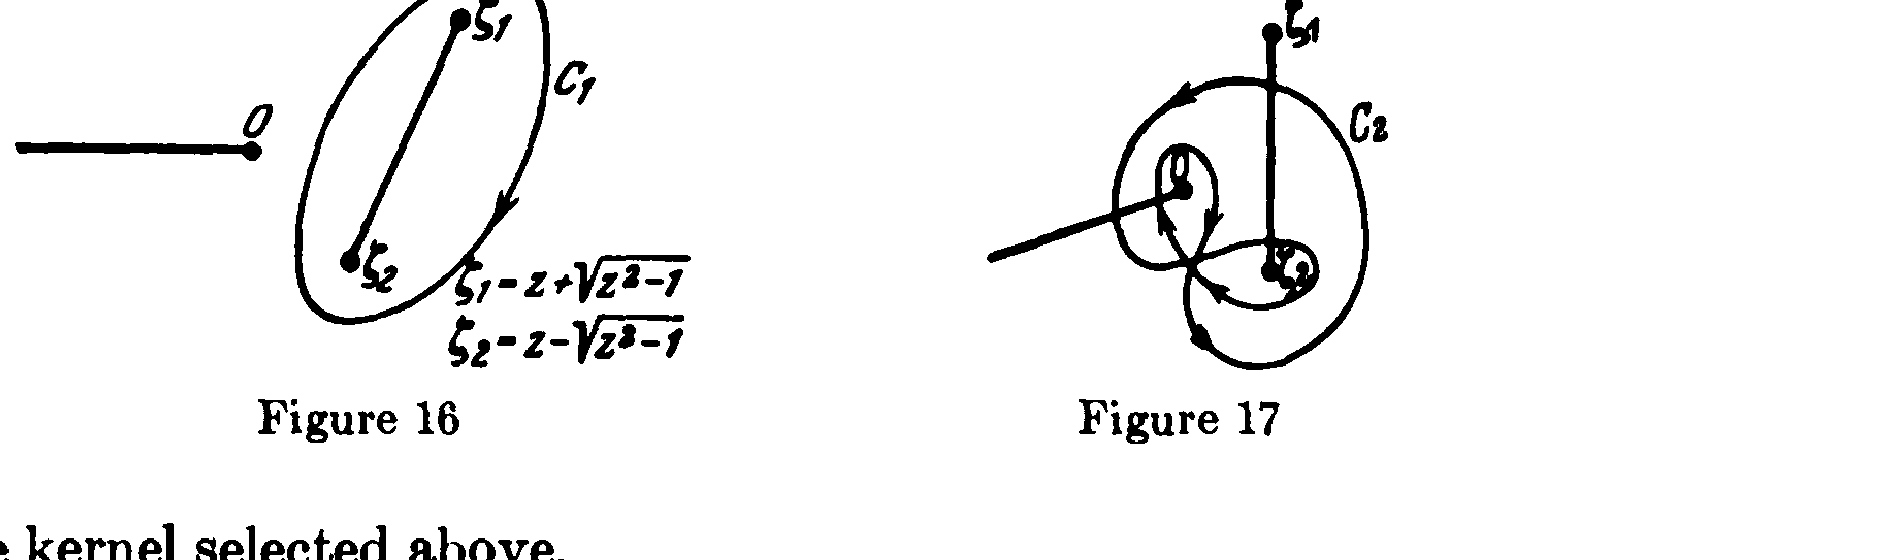
\includegraphics[width=0.78\textwidth]{figures/ch07_fig16_17.png}
\end{center}

The kernel selected above,
\[
K(z,\zeta)=\frac1{\sqrt{1-2z\zeta+\zeta^2}},
\]
as well as any other which satisfies equation (57), is a generating function of the Legendre equation. For, the coefficient $u_n(z)$ in the series expansion
\[
K(z,\zeta)=\sum_{0}^{\infty}u_n(z)\zeta^n
\]
of such a kernel is an integral of the above form,
\[
u_n(z)=\frac1{2\pi i}\oint\frac{K(z,\zeta)}{\zeta^{n+1}}\,d\zeta;
\]
since the path of integration is closed, $u_n(z)$ is a solution of equation (56) for $\lambda=n$.

\subsection{Tchebycheff Functions}
In the case of Tchebycheff's equation
\begin{equation}\tag{59}
L[u]=(1-z^2)u''-zu'=-\lambda^2u,
\end{equation}
we take $K$ to be a solution of the differential equation
\begin{equation}\tag{60}
(1-z^2)K_{zz}-zK_z+\zeta(\zeta K_\zeta)_\zeta=0;
\end{equation}
for example, we take $K(z,\zeta)=1-\zeta^2/(1-2z\zeta+\zeta^2)$, which leads to

% --- printed p.508 ---
solutions of the form
\begin{equation}\tag{61}
\begin{aligned}
P_\lambda(z)&=\frac1{2\pi i}\int_{C_1}
\frac{1-\zeta^2}{1-2z\zeta+\zeta^2}\,\zeta^{-\lambda-1}\,d\zeta,\\
Q_\lambda(z)&=\frac1{2\pi i}\int_{C_2}
\frac{1-\zeta^2}{1-2z\zeta+\zeta^2}\,\zeta^{-\lambda-1}\,d\zeta.
\end{aligned}
\end{equation}
Here $C_1$ and $C_2$ are closed curves on the Riemann surface of the integrand and enclose the zeros of the denominator
\[
\zeta_1=z+\sqrt{z^2-1};\qquad \zeta_2=z-\sqrt{z^2-1}
\]
(see Figure 18). Application of Cauchy's integral theorem yields
\begin{equation}\tag{62}
\begin{aligned}
P_\lambda(z)&=(z+\sqrt{z^2-1})^\lambda,\\
Q_\lambda(z)&=(z-\sqrt{z^2-1})^\lambda.
\end{aligned}
\end{equation}

\begin{center}
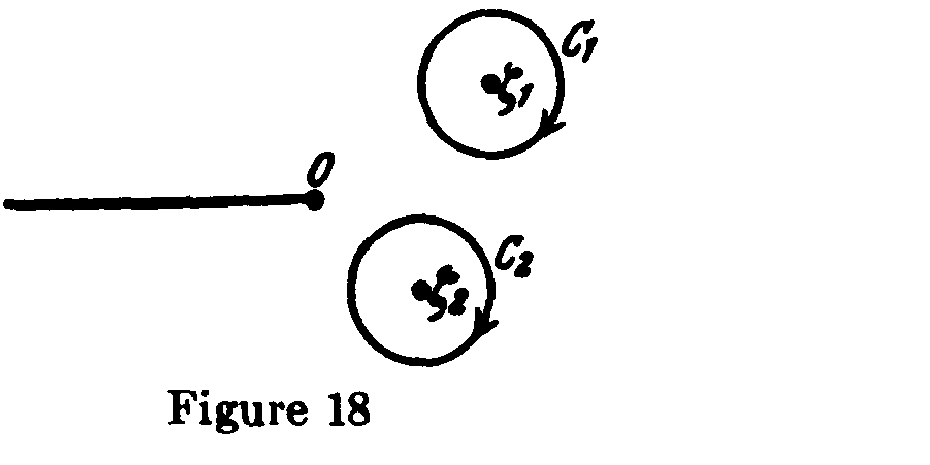
\includegraphics[width=0.33\textwidth]{figures/ch07_fig18.png}
\end{center}

The sum
\[
T_\lambda(z)=\frac1{2^\lambda}(P_\lambda(z)+Q_\lambda(z))
=\frac{(z+\sqrt{z^2-1})^\lambda+(z-\sqrt{z^2-1})^\lambda}{2^\lambda},
\]
which is represented also by the integral
\[
T_\lambda(z)=\frac1{2^\lambda}\frac1{2\pi i}\int_C
\frac{1-\zeta^2}{1-2z\zeta+\zeta^2}\,\zeta^{-\lambda-1}\,d\zeta
\]
in which $C$ now encloses both points $\zeta_1$ and $\zeta_2$, goes over into the $n$-th Tchebycheff polynomial for $\lambda=n$.

\subsection{Hermite Functions}
In the case of the Hermite equation
\begin{equation}\tag{63}
L[u]=u''-2zu'=-2\lambda u
\end{equation}
we require $K$ to satisfy equation
\begin{equation}\tag{64}
K_{zz}-2zK_z+2\zeta K_\zeta=0,
\end{equation}
which has the function $e^{2z\zeta-\zeta^2}$ as a solution. If for $C$ we take one of the curves represented in Figure 19, we obtain the solutions
\begin{equation}\tag{65}
\begin{aligned}
P_\lambda(z)&=\frac1{\pi i}\int_{C_1}\frac{e^{-\zeta^2+2z\zeta}}{\zeta^{\lambda+1}}\,d\zeta,\\
Q_\lambda(z)&=\frac1{\pi i}\int_{C_2}\frac{e^{-\zeta^2+2z\zeta}}{\zeta^{\lambda+1}}\,d\zeta.
\end{aligned}
\end{equation}

% --- printed p.509 ---
Their arithmetic mean,
\[
H_\lambda(z)=\tfrac12(P_\lambda(z)+Q_\lambda(z)),
\]
in other words, the integral
\[
H_\lambda(z)=\frac1{2\pi i}\int_C\frac{e^{-\zeta^2+2z\zeta}}{\zeta^{\lambda+1}}\,d\zeta,
\]
where $C$ is the loop in Figure 21, becomes the Hermite polynomial $H_n(z)$ for $\lambda=n$.

If $\Re(\lambda)<0$, we can contract the path of integration to the origin and obtain as solutions---up to factors independent of $z$---the integrals
\begin{equation}\tag{66}
\int_0^\infty\frac{e^{-\zeta^2+2z\zeta}}{\zeta^{\lambda+1}}\,d\zeta
\end{equation}
and
\begin{equation}\tag{67}
\int_{-\infty}^0\frac{e^{-\zeta^2+2z\zeta}}{\zeta^{\lambda+1}}\,d\zeta.
\end{equation}

\begin{center}
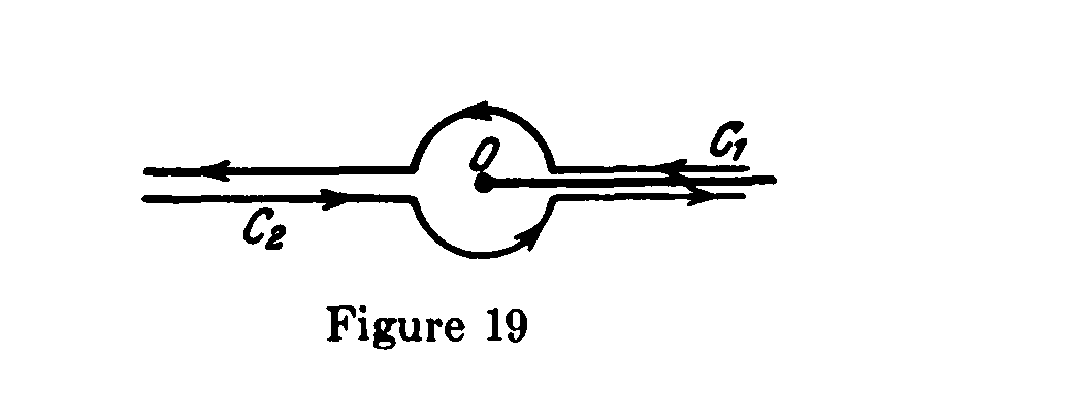
\includegraphics[width=0.43\textwidth]{figures/ch07_fig19.png}
\end{center}

\subsection{Laguerre Functions}
Correspondingly, in the Laguerre equation
\begin{equation}\tag{68}
L[u]=zu''+(1-z)u'=-\lambda u
\end{equation}
we impose on $K(z,\zeta)$ the partial differential equation
\begin{equation}\tag{69}
zK_{zz}+(1-z)K_z+\zeta K_\zeta=0
\end{equation}
and arrive at integrals of the form
\begin{equation}\tag{70}
\int_C\frac{e^{-z\zeta/(1-\zeta)}}{1-\zeta}\,\zeta^{-\lambda-1}\,d\zeta.
\end{equation}
In the choice of the path of integration $C$, it must be noted that the integrand has an essential singularity at the point $\zeta=1$. In particular if we take for $C$ the curve shown in Figure 20, the integral
\begin{equation}\tag{71}
L_\lambda(z)=\frac1{2\pi i}\int_C\frac{e^{-z\zeta/(1-\zeta)}}{1-\zeta}\,\zeta^{-\lambda-1}\,d\zeta
\end{equation}
represents solutions which are essentially identical with the Laguerre polynomials in the case $\lambda=n$.

By means of the transformation
\[
u=\frac\zeta{1-\zeta},
\]

% --- printed p.510 ---
(71) acquires the form
\begin{equation}\tag{72}
L_\lambda(z)=\frac{1}{2\pi i}\int_C\frac{e^{-uz}}{u^{\lambda+1}}(1+u)^\lambda\,du;
\end{equation}
now $C$ denotes the path in Figure 21.

Furthermore, we note that, as in the case of Legendre's equation, every solution of the partial differential equation associated with each equation discussed here can be considered as a \emph{generating function} of a family of solutions of the original differential equation. In particular, the special kernels we have used define, by their power series expansions, the Tchebycheff, Hermite, and Laguerre polynomials.

\begin{center}
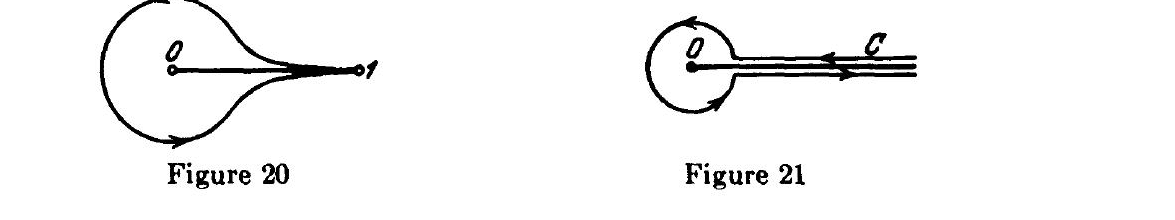
\includegraphics[width=0.76\textwidth]{figures/ch07_fig20_21.png}
\end{center}

\section{Laplace Spherical Harmonics}
The Laplace spherical harmonics $Y_n(\theta,\varphi)$ were introduced in Ch. V, \S8, p. 314 as the everywhere-regular eigenfunctions, corresponding to the eigenvalues $\lambda=n(n+1)$, of the differential equation
\begin{equation}\tag{73}
\Delta^*Y+\lambda Y
=\frac{1}{\sin^2\theta}Y_{\varphi\varphi}
+\frac{1}{\sin\theta}(\sin\theta\,Y_\theta)_\theta
+\lambda Y=0
\end{equation}
on the sphere. We see that the functions $r^nY_n=U_n$ are then polynomials in the rectangular coordinates $x,y,z$ which satisfy the differential equation $\Delta U=0$ and are homogeneous of degree $n$. Conversely, every integral rational solution $U_n$ of the differential equation $\Delta U=0$ which is homogeneous of degree $n$ becomes a Laplace spherical harmonic when divided by $r^n$. Since a polynomial which is homogeneous of degree $n$ has $(n+1)(n+2)/2$ coefficients, and since the condition $\Delta U_n=0$ determines $(n-1)n/2$ linear homogeneous relations between these coefficients---for, $\Delta U_n$ is homogeneous of $(n-2)$-nd degree---, the $U_n$ have at least
\[
\frac{(n+1)(n+2)}{2}-\frac{(n-1)n}{2}=2n+1
\]

% --- printed p.511 ---
independent coefficients; therefore there must be at least $2n+1$ linearly independent spherical harmonics of $n$-th order.

In this paragraph it will be shown that the aforementioned conditions are mutually independent, so that there exist precisely $2n+1$ linearly independent spherical harmonics of $n$-th order. It will be shown also that these functions $Y_n$ really represent all the eigenfunctions of our eigenvalue problem, and hence that the values $\lambda=n(n+1)$ represent all the eigenvalues. Finally, these functions will be expressed explicitly in terms of associated Legendre functions, with which we are familiar from \S3 and Ch. V, \S10, 2, p. 327. We begin with the last point.

\subsection{Determination of $2n+1$ Spherical Harmonics of $n$-th Order}
We again obtain special spherical harmonics by means of the familiar trial substitution $Y(\theta,\varphi)=p(\varphi)q(\theta)$. We make this substitution in equation (73) for $\lambda=n(n+1)$, and denote differentiation with respect to $\varphi$ by a prime, and differentiation with respect to $\theta$ by a dot; equation (73) then becomes
\[
\frac{p''(\varphi)}{p(\varphi)}
=-\frac{(\sin\theta\,\dot q)^{\boldsymbol\cdot}\sin\theta}{q}
-n(n+1)\sin^2\theta=-\rho,
\]
in which $\rho$ must be a constant. Thus we obtain for $q$ the equation
\[
(\sin\theta\,\dot q)^{\boldsymbol\cdot}
+\left(n(n+1)\sin\theta-\frac{\rho}{\sin\theta}\right)q=0,
\]
in which the parameter $\rho$ must be determined in such a way that a solution exists which is regular for $\theta=0$ and $\theta=\pi$. Substituting $z=\cos\theta$, and denoting differentiation with respect to $z$ by a prime, this equation immediately becomes
\[
\bigl((1-z^2)q'\bigr)'
+\left(n(n+1)-\frac{\rho}{1-z^2}\right)q=0
\]
with the boundary condition of regularity for $z=+1$ and $z=-1$; this problem is familiar to us, in a somewhat different form, from Ch. V, \S10, 2, p. 327. We already know the solutions $\rho=h^2$ and $q=P_{n,h}(z)$, where $P_{n,h}(z)$ is the Legendre function of $h$-th order, and
\[
P_{n,h}=(1-z^2)^{h/2}\frac{d^h}{dz^h}P_n(z);
\]
$h$ can assume the values $0,1,2,\ldots,n$. Since $p''(\varphi)+h^2p(\varphi)=0$, $p$ is given as $a_h\cos h\varphi+b_h\sin h\varphi$; since $Y=pq$, we at once obtain
\[
Y(\theta,\varphi)=(a_h\cos h\varphi+b_h\sin h\varphi)P_{n,h}(\cos\theta)
\]

% --- printed p.512 ---
as a solution of (73). Therefore the function
\begin{equation}\tag{74}
Y_n=\frac{a_{n,0}}{2}P_n(\cos\theta)
+\sum_{h=1}^{n}(a_{n,h}\cos h\varphi+b_{n,h}\sin h\varphi)P_{n,h}(\cos\theta)
\end{equation}
is a spherical harmonic of dimension $n$ depending upon $2n+1$ arbitrary linear parameters. It will soon be apparent that this function is the most general possible. The functions $\cos h\varphi\,P_{n,h}(\cos\theta)$, $\sin h\varphi\,P_{n,h}(\cos\theta)$ are all linearly independent, since they are mutually orthogonal; they will be called \emph{symmetric spherical harmonics of order $n$}.

\subsection{Completeness of the System of Functions}
From earlier theorems we see at once that the $2n+1$ functions $\cos h\varphi\,\allowbreak P_{n,h}(\cos\theta)$, $\sin h\varphi\,\allowbreak P_{n,h}(\cos\theta)$ form a complete orthogonal system of functions on the sphere. The functions $\sin h\varphi$, $\cos h\varphi$ form a complete system in the variable $\varphi$, and the functions $P_{n,h}(z)$ for every $h$ form a complete system in $z$ because the system of all eigenfunctions of an eigenvalue problem is always complete (see Ch. VI, \S3, 1). In order to prove that the system of functions is complete, we need only recall the theorem of Ch. II, \S1, 6, which contains a general rule for constructing a complete system of functions in two variables from two complete systems in one variable.

From this result it follows immediately that equation (73) has no eigenfunctions other than those indicated, and thus can have no eigenvalues except the values $n(n+1)$. All the questions which were raised above have thus been answered. (Note that this constitutes a transcendental proof of the algebraic fact that there exist precisely $2n+1$ linearly independent functions $Y_n$.)

This fact may, of course, be proved easily from the standpoint of algebra alone. Consider any polynomial $u$ of $x,y,z$ which is homogeneous of degree $n$:
\[
u=\sum a_{rst}x^ry^sz^t\qquad(r+s+t=n).
\]
Then every coefficient $a_{rst}$ may be represented, up to a constant factor, as a derivative of the form $\partial^n u/\partial x^r\partial y^s\partial z^t$. If $\Delta u=0$, every derivative of the form $\partial^m u/\partial x^\alpha\partial y^\beta\partial z^\gamma$ can be written in such a way that differentiation with respect to $x$ occurs no more than once; we use the differential equation $u_{xx}=-u_{yy}-u_{zz}$ to eliminate all derivatives of $u$ with respect to $x$ of order higher than one (for example, $\partial^3u/\partial x^2\partial y=-\partial^3u/\partial y^3-\partial^3u/\partial z^2\partial y$). Thus, if $\Delta u=0$, all coefficients of $u$ are linear combinations of the $2n+1$ coefficients
\[
a_{0,0,n},a_{0,1,n-1},\ldots,a_{0,n,0};\qquad
a_{1,0,n-1},a_{1,1,n-2},\ldots,a_{1,n-1,0},
\]
which may be chosen arbitrarily.

% --- printed p.513 ---
\subsection{Expansion Theorem}
Since the functions (74) represent all the eigenfunctions of our problem, our earlier theorems (see e.g. Ch. V, \S14, 5) imply that every function $g(\theta,\varphi)$ which is continuous together with its derivatives up to the second order on the sphere may be expanded in an absolutely and uniformly convergent series in terms of the spherical harmonics
\[
g(\theta,\varphi)=\sum_{n=0}^{\infty}\left[a_{n,0}P_n(\cos\theta)
+\sum_{h=1}^{n}(a_{n,h}\cos h\varphi+b_{n,h}\sin h\varphi)P_{n,h}(\cos\theta)\right],
\]
where, in view of the formulas of Ch. V, \S10, p. 327, the coefficients $a_{n,0}$, $a_{n,h}$, $b_{n,h}$ are determined from the relations
\begin{equation}\tag{75}
\begin{aligned}
a_{n,0}&=\frac{2n+1}{4\pi}\int_{-\pi}^{\pi}\int_0^\pi
 g(\theta,\varphi)P_n(\cos\theta)\sin\theta\,d\theta\,d\varphi,\\
a_{n,h}&=\frac{2n+1}{2\pi}\frac{(n-h)!}{(n+h)!}
\int_{-\pi}^{\pi}\int_0^\pi g(\theta,\varphi)P_{n,h}(\cos\theta)\cos h\varphi\sin\theta\,d\theta\,d\varphi,\\
b_{n,h}&=\frac{2n+1}{2\pi}\frac{(n-h)!}{(n+h)!}
\int_{-\pi}^{\pi}\int_0^\pi g(\theta,\varphi)P_{n,h}(\cos\theta)\sin h\varphi\sin\theta\,d\theta\,d\varphi.
\end{aligned}
\end{equation}
Extension of this result to more general functions $g(\theta,\varphi)$ need not concern us here.

\subsection{The Poisson Integral}
We can now write the solution of the boundary value problem of potential theory for a sphere of radius 1 with boundary values $g(\theta,\varphi)$ explicitly in the form
\[
u=\sum_{n=0}^{\infty}r^n\left[a_{n,0}P_n(\cos\theta)
+\sum_{h=1}^{n}(a_{n,h}\cos h\varphi+b_{n,h}\sin h\varphi)P_{n,h}(\cos\theta)\right].
\]
If we introduce the integral representations (75), we can interchange summation and integration since the convergence is uniform for $r\le r_0<1$. The summation may then be carried out in closed form; in doing this it is easiest to assume at first $\theta=0$, $\varphi=0$, and then to note that the result must hold for an arbitrary point $\theta,\varphi$, since any point on the sphere may be chosen as the north pole.

Since $P_n(1)=1$, $P_{n,h}(1)=0$ $(h=1,2,\ldots,n)$, we obtain
\[
4\pi u(r,0,0)=\int_{-\pi}^{\pi}\int_0^\pi
\left\{\sum_{n=0}^{\infty}(2n+1)r^nP_n(\cos\theta)\right\}
g(\theta,\varphi)\sin\theta\,d\theta\,d\varphi;
\]
here the sum may be obtained in closed form by using the relation
\[
\sum_{n=0}^{\infty}(2n+1)h^nP_n(z)=\frac{1-h^2}{(1-2hz+h^2)^{3/2}},
\]

% --- printed p.514 ---
which can be easily derived from the equation of definition
\[
\sum_{n=0}^{\infty}h^nP_n(z)=(1-2hz+h^2)^{-1/2}
\]
with the aid of the recursion formula (49). After carrying out the summation and again thinking of the pole of the sphere as displaced, we can write the result with complete generality in the form
\begin{equation}\tag{76}
4\pi u(r,\theta,\varphi)
=(1-r^2)\int_{-\pi}^{\pi}\int_0^\pi
\frac{g(\theta',\varphi')\sin\theta'\,d\theta'\,d\varphi'}
{\left\{r^2-2r[\cos\theta\cos\theta'+\sin\theta\sin\theta'\cos(\varphi-\varphi')]+1\right\}^{3/2}}.
\end{equation}
This so-called \emph{Poisson integral} expresses the potential function at interior points in terms of its boundary values; it no longer contains any explicit reference to the spherical harmonics. In Volume II we shall return to this integral in the framework of potential theory.

\subsection{The Maxwell-Sylvester Representation of Spherical Harmonics}
An entirely different representation for the spherical harmonics, connected with the physical meaning of a potential, was given by Maxwell.\footnote{A Treatise on Electricity and Magnetism, Vol. 1, pp. 179--214, 2nd ed., Clarendon Press, Oxford, 1881.} In this section we shall investigate the properties of spherical functions in connection with Maxwell's basic ideas and a supplementary remark of Sylvester, and thus arrive at a new development of our theory.

We begin with the potential $1/r=1/\sqrt{x^2+y^2+z^2}$ corresponding to a unit mass concentrated at the origin, and note that every derivative
\[
v=\frac{\partial^n u}{\partial x^\alpha\partial y^\beta\partial z^\gamma}
\qquad(n=\alpha+\beta+\gamma)
\]
of a potential function $u$ is again a solution of the potential equation $\Delta v=0$, since from $\Delta u=0$ we obtain by differentiation
\[
0=\frac{\partial}{\partial x}\Delta u=\Delta\frac{\partial u}{\partial x},
\]
etc. Hence, if $a,b,c$ are constants, the function
\[
a\frac{\partial(1/r)}{\partial x}
+b\frac{\partial(1/r)}{\partial y}
+c\frac{\partial(1/r)}{\partial z}
\]

% --- printed p.515 ---
is also a potential function. Using the symbolic linear form
\[
L=a\frac{\partial}{\partial x}+b\frac{\partial}{\partial y}+c\frac{\partial}{\partial z},
\]
we can write it in the form $L\frac1r$ or in the form
\[
\alpha\frac{\partial(1/r)}{\partial\nu},
\]
where $\alpha=\sqrt{a^2+b^2+c^2}$ and $\partial/\partial\nu$ stands for differentiation in that direction $\nu$ whose direction cosines are proportional to $a,b,c$.\footnote{If complex values are admitted for the $a,b,c$, necessary precautions must naturally be taken in the case of those triples for which $a^2+b^2+c^2=0$.} Physically, this potential corresponds to a dipole of moment $\alpha$ and direction $\nu$. More generally, in the expression
\begin{equation}\tag{77}
u=C\frac{\partial^n(1/r)}{\partial\nu_1\partial\nu_2\cdots\partial\nu_n}
=CL_1L_2\cdots L_n\frac1r
\end{equation}
we obtain a potential which corresponds to a ``multipole'' with the axes $\nu_1,\nu_2,\ldots,\nu_n$. The $L_i$ denote linear forms in the operators $\partial/\partial x$, $\partial/\partial y$, $\partial/\partial z$, and their coefficients $a_i,b_i,c_i$ define the axis directions $\nu_i$. It is easily seen that the potential $u$ has the form
\begin{equation}\tag{78}
u=U_n(x,y,z)r^{-2n-1},
\end{equation}
where $U_n$ is a homogeneous polynomial of degree $n$ in $x,y,z$. The function $U_n$ itself satisfies the potential equation $\Delta U_n=0$, as is seen from the following general theorem: \emph{If $u(x,y,z)$ is a solution of the potential equation, then $(1/r)u(x/r^2,y/r^2,z/r^2)$ is also a solution.}\footnote{The proof of this theorem is obtained immediately from the polar coordinate form of the potential equation (see Ch. IV, \S8, 2).} For $r=1$, such functions $U_n(x,y,z)$ according to our earlier definitions (Ch. V, \S9, 1) are spherical harmonics of order $n$.

Since each of the $n$ directions occurring in (77) is determined by two parameters, and an additional arbitrary constant factor appears in the potential $u$, there are $2n+1$ arbitrary constants in all. It may be conjectured, therefore, that all the spherical harmonics of order $n$ can in fact be represented in the form (77). We shall prove

% --- printed p.516 ---
this rigorously by first representing the $2n+1$ linearly independent symmetric spherical harmonics $P_{n,h}(\cos\theta)\sin h\varphi$, $P_{n,h}(\cos\theta)\cos h\varphi$ in terms of multipole potentials. Subsequently it will follow that every $n$-th order spherical harmonic is given by a sum of multipole potentials. Finally, we shall show that every sum of several such multipole potentials is equal to the potential of a single multipole, which can be obtained by means of a simple geometric construction.

The $2n+1$ symmetric spherical harmonics of subsection 1 are obtained easily by considering symmetric multipoles. Let $n$ axes with the directions $\nu_1,\nu_2,\ldots,\nu_n$ be arranged symmetrically in the $x,y$-plane in such a way that any two consecutive axes form the angle $2\pi/n$ with each other. If we set
\begin{equation}\tag{79}
\frac{\partial^n(1/r)}{\partial\nu_1\partial\nu_2\cdots\partial\nu_n}
=u_n=U_nr^{-2n-1}
\end{equation}
and note that the left side is invariant with respect to rotations of the sphere about the $z$-axis through the angle $2\pi/n$, we see at once that the $n$-th order spherical harmonic
\[
u_nr^{n+1}=U_nr^{-n}=Y_n(\theta,\varphi),
\]
which certainly does not vanish identically,\footnote{That no multipole potential can vanish identically will be proved on page 519.} has the period $2\pi/n$ when considered as a function of $\varphi$. By subsection 3 every spherical harmonic of order $n$ permits the representation
\[
\sum_{h=0}^{n}(a_{n,h}\cos h\varphi+b_{n,h}\sin h\varphi)P_{n,h}(\cos\theta).
\]
It follows that $Y_n(\theta,\varphi)$ has the form
\begin{equation}\tag{80}
\begin{aligned}
Y_n(\theta,\varphi)
&=[a_{n,n}\cos n\varphi+b_{n,n}\sin n\varphi]P_{n,n}(\cos\theta)
+a_{n,0}P_{n,0}(\cos\theta)\\
&=\alpha\cos n(\varphi-\varphi_0)P_{n,n}(\cos\theta)+\beta P_{n,0}(\cos\theta).
\end{aligned}
\end{equation}
The two terms in (80) are the only ones which are periodic in $\varphi$ with period $2\pi/n$. The term $P_{n,0}(\cos\theta)$ can be expressed separately in terms of a derivative of $r^{-1}$. We have
\begin{equation}\tag{80'}
\frac{\partial^n}{\partial z^n}\left(\frac1r\right)
=\frac{(-1)^n n!}{r^{n+1}}P_n(\cos\theta).
\end{equation}

% --- printed p.517 ---
The fact that the right side in (80') is a multiple of $r^{-n-1}P_{n,0}(\cos\theta)$ follows immediately from the remarks made above. The calculation of the constant factor can be carried out by induction, using the recursion formulas (49).

In order to obtain a multipole representation for the remaining spherical harmonics of $n$-th order, we note that because of (80) the potential $u_n$ can be decomposed as follows:
\[
u_n=f(x,y)g\left(\frac zr\right)r^{-n-1},
\]
where $f(x,y)=\alpha\cos n(\varphi-\varphi_0)$, $f(0,0)=0$. We replace $n$ by $h$ in this expression and then differentiate $n-h$ times with respect to $z$. The resulting potential function $u_{n,h}$ again has the form
\[
u_{n,h}=f(x,y)g\left(\frac zr\right)r^{-n-1},
\]
from which we conclude that the $n$-th order spherical harmonic
\[
Y_n(\theta,\varphi)=u_{n,h}r^{n+1}
\]
must have the form $\alpha\cos h(\varphi-\varphi_0)\omega(\theta)$. Therefore by subsection 1 it necessarily has the form
\begin{equation}\tag{81}
\text{const.}\times\cos h(\varphi-\varphi_0)P_{n,h}(\cos\theta).
\end{equation}
Conversely, since one of the axes can be chosen arbitrarily, every function of this family is obtained by our procedure.

Since according to subsection 2 every spherical harmonic of order $n$ may be expressed as a sum of $2n+1$ spherical harmonics of the form (81), it follows at once that we obtain every $n$-th order spherical harmonic by forming sums of multipole potentials
\begin{equation}\tag{82}
u=\sum_{i+j+k=n}a_{ijk}
\frac{\partial^n(1/r)}{\partial x^i\partial y^j\partial z^k}.
\end{equation}
That, conversely, every such sum is a spherical harmonic of order $n$ is obvious according to page 510. In fact, any particular spherical harmonic is represented infinitely often when we let the coefficients $a_{ijk}$ run through all possible values. We shall now elaborate this point.

We first prove that every sum of the above form is the potential

% --- printed p.518 ---
of a single multipole with suitable axes. To do this we make use of a symbolic notation, considering the homogeneous polynomial of $n$-th degree
\[
H(\xi,\eta,\zeta)=\sum_{i+k+l=n}a_{ikl}\xi^i\eta^k\zeta^l
\]
and writing our potential in the form $H/r$, in which we replace the variables $\xi,\eta,\zeta$ in $H$ by the differentiation symbols $\partial/\partial x$, $\partial/\partial y$, $\partial/\partial z$. Since with this meaning of $\xi,\eta,\zeta$ the function $(\xi^2+\eta^2+\zeta^2)/r$ is identically zero, we have $H/r=H_1/r$ provided the difference $H-H_1$, as a polynomial in the indeterminates $\xi,\eta,\zeta$, can be expressed in the form $Q\cdot(\xi^2+\eta^2+\zeta^2)$, where $Q$ denotes a homogeneous polynomial of $(n-2)$-nd degree in $\xi,\eta,\zeta$.

At this point we need a simple theorem employed by Sylvester:\footnote{J. J. Sylvester, Note on Spherical Harmonics, Phil. Mag., Vol. 2m, 1876, pp. 291--307 and 400. Collected Mathematical Papers, Vol. 3, pp. 37--51, Cambridge University Press, Cambridge, 1909.} \emph{Given any homogeneous polynomial of $n$-th degree $H(\xi,\eta,\zeta)$, we can determine $n$ linear forms $L_1,L_2,\ldots,L_n$ and a polynomial $Q(\xi,\eta,\zeta)$ of degree $n-2$ in such a way that a relation of the form}
\[
H=C\cdot L_1L_2\cdots L_n+Q\cdot(\xi^2+\eta^2+\zeta^2)
\]
\emph{holds. If $H$ is real, the linear forms $L_1,L_2,\ldots,L_n$ are determined uniquely, up to constant factors, by the condition that their coefficients be real.} The proof of this theorem, as well as the geometric characterization of the forms $L_i$, will be postponed to the end of the section so as not to interrupt the train of thought. Our assertion concerning the representation of the potential (82) by a single multipole follows at once from Sylvester's theorem. For, if $\nu_i$ denotes the axial direction perpendicular to the plane $L_i=0$, we obtain
\[
u=H\frac1r=C\frac{\partial^n(1/r)}{\partial\nu_1\partial\nu_2\cdots\partial\nu_n},
\]
which furnishes the desired representation.

Our theory is now outlined in its essential points. We shall give our discussion a somewhat different turn which avoids dependence on the results of subsections 1 and 2 and puts more stress on the

% --- printed p.519 ---
purely algebraic nature of our theorems, although at the same time it relaxes the connection with the explicit representations. First we remark that two functions $H/r$ and $H_1/r$ are identical if and only if the difference $H^*(\xi,\eta,\zeta)=H(\xi,\eta,\zeta)-H_1(\xi,\eta,\zeta)$ is divisible by $\xi^2+\eta^2+\zeta^2$. As already pointed out, the first part of the assertion is obvious. In order to prove the second part, we must show that a relation $H^*/r=0$ implies that the homogeneous polynomial $H^*(\xi,\eta,\zeta)$ is divisible by $\xi^2+\eta^2+\zeta^2$.\footnote{See the work by A. Ostrowski referred to on p. 521, footnote 2.} Now by Sylvester's theorem
\begin{equation}\tag{83}
H^*=C\cdot L_1^*L_2^*\cdots L_n^*+Q^*\cdot(\xi^2+\eta^2+\zeta^2),
\end{equation}
where $L_1^*,L_2^*,\ldots,L_n^*$ denote linear forms which, in the case of real $H^*$, may be supposed real. If one of the linear forms $L_i^*$ vanishes identically, our assertion is clear. However, if none of the linear forms vanishes identically, we have
\[
H^*\frac1r=C\cdot L_1^*L_2^*\cdots L_n^*\frac1r
=C\frac{\partial^n(1/r)}{\partial\nu_1^*\partial\nu_2^*\cdots\partial\nu_n^*},
\]
and the multipole potential on the right side, because of the singularity at the origin, can vanish in the whole space only if $C=0$. Otherwise, for suitable $m$, $0\le m<n$, we would have
\[
\frac{\partial^m(1/r)}{\partial\nu_1\cdots\partial\nu_m}=v_m\ne0,
\qquad
\frac{\partial v_m}{\partial\nu_{m+1}}=0;
\]
hence $v_m$ would have to have constant values on every parallel to the axis $\nu_{m+1}$, which is impossible because of the singularity at the origin. We thus have
\[
H^*(\xi,\eta,\zeta)=Q^*(\xi,\eta,\zeta)(\xi^2+\eta^2+\zeta^2),
\]
which is what we wished to prove.

Clearly, every homogeneous function $H(\xi,\eta,\zeta)$ of degree $n$ can be expressed in one and only one way in the form
\begin{equation}\tag{84}
H(\xi,\eta,\zeta)=G_n(\eta,\zeta)+\xi G_{n-1}(\eta,\zeta)
+(\xi^2+\eta^2+\zeta^2)\,Q(\xi,\eta,\zeta).
\end{equation}
Here $G_n$ denotes a homogeneous function of degree $n$ in $\eta,\zeta$ alone, $G_{n-1}$ a homogeneous function of degree $(n-1)$, and $Q$ a homogeneous

% --- printed p.520 ---
function of degree $(n-2)$. The difference between two functions $H(\xi,\eta,\zeta)$ and $\bar H(\xi,\eta,\zeta)$ of degree $n$ is divisible by $\xi^2+\eta^2+\zeta^2$ if and only if the associated functions $G_n,G_{n-1},\bar G_n,\bar G_{n-1}$ satisfy the relations
\[
G_n=\bar G_n,\qquad G_{n-1}=\bar G_{n-1}
\]
identically. Since we have $2n+1$ coefficients at our disposal in the functions $G_n$ and $G_{n-1}$, the lemma just proved shows that we have precisely $2n+1$ linearly independent potentials in the form $H/r$. Hence we obtain every spherical harmonic of degree $n$ as a sum of potentials of multipoles. In order actually to obtain the representation of the spherical functions in this form one must use, in addition to this pure existence proof, an argument analogous to that carried out above.

Finally we shall prove Sylvester's theorem using a simple idea from algebraic geometry. By Bezout's theorem, the $n$-th degree cone $H(\xi,\eta,\zeta)=0$ in $\xi,\eta,\zeta$-space intersects the absolute cone $\xi^2+\eta^2+\zeta^2=0$ in precisely $2n$ edges; all multiple intersections are correctly weighted. We connect the $2n$ edges by means of $n$ planes given by the equations
\[
L_i(\xi,\eta,\zeta)=a_i\xi+b_i\eta+c_i\zeta=0\qquad(i=1,2,\ldots,n)
\]
in such a way that each plane contains two of the edges and every edge is accounted for once. Multiple edges appear according to their multiplicity.\footnote{We can make the meaning of this rule more precise without referring to the difficult general algebraic elimination theory: We uniformize the form $\xi^2+\eta^2+\zeta^2=0$ by setting
\[
\xi=\frac{1-t^2}{1+t^2},\qquad \eta=\frac{2t}{1+t^2},\qquad \zeta=i=\sqrt{-1}.
\]
A homogeneous function $H(\xi,\eta,\zeta)$ of degree $n$ is then transformed by this substitution into a rational function $H^*(t)$ of degree $2n$, whose zeros determine the common edges of the cones $H(\xi,\eta,\zeta)=0$ and $\xi^2+\eta^2+\zeta^2=0$. We shall say that a common edge of these cones counts $k$-fold if on it $H^*(t)$, as a function of $t$, has a precisely $k$-fold zero. The linear forms $L_1,L_2,\ldots,L_n$ are now to be chosen in such a way that every $k$-fold curve of intersection of the cone $H=0$ with the absolute cone is also a $k$-fold edge of intersection of the family of planes $L_1,L_2,\ldots,L_n=0$. That this rule may be realized in every case is easily seen.} We now consider the bundle of cones of $n$-th order
\[
\lambda H+\mu L_1L_2\cdots L_n=0
\]

% --- printed p.521 ---
containing the two parameters $\lambda$ and $\mu$. Every cone of this bundle intersects the absolute cone in the $2n$ given fixed edges. Selecting any one edge of the absolute conic not one of the above fixed $2n$ edges, we determine the ratio $\lambda/\mu$ in such a way that the $n$-th degree cone
\[
\lambda H+\mu L_1L_2\cdots L_n=0
\]
passes also through this edge, which is certainly possible and which leads to a value for $\lambda/\mu$ different from zero and infinity. The new cone of degree $n$ then has more than $2n$ lines of intersection in common with a cone of second degree, which is impossible unless it contains the cone of second degree completely. This case arises if and only if the left side of the equation contains the expression $\xi^2+\eta^2+\zeta^2$ as a factor,\footnote{The first part of the assertion is obvious. The second is proved most simply by writing the given form, in accordance with (84), as
\[
G_n(\eta,\zeta)+\xi G_{n-1}(\eta,\zeta)+(\xi^2+\eta^2+\zeta^2)Q(\xi,\eta,\zeta).
\]
Now if $\eta,\zeta$ is any pair of values for which $\eta^2+\zeta^2\ne0$, the two equations
\[
0=G_n(\eta,\zeta)+\sqrt{-(\eta^2+\zeta^2)}\,G_{n-1}(\eta,\zeta)
\]
and
\[
0=G_n(\eta,\zeta)-\sqrt{-(\eta^2+\zeta^2)}\,G_{n-1}(\eta,\zeta)
\]
hold simultaneously. We conclude at once $G_n(\eta,\zeta)=G_{n-1}(\eta,\zeta)=0$. Thus $G_n$ and $G_{n-1}$ vanish for all pairs of values $\eta,\zeta$ with $\eta^2+\zeta^2\ne0$; hence they vanish identically in $\eta$ and $\zeta$.} i.e. if
\[
\lambda H+\mu L_1L_2\cdots L_n=Q\cdot(\xi^2+\eta^2+\zeta^2).
\]
The proof of Sylvester's theorem is now complete.\footnote{This algebraic theorem was used by Sylvester, loc. cit., without proof. The necessity of obtaining a proof for it was indicated by A. Ostrowski. See Ostrowski, Mathematische Miszellen, I, Die Maxwellsche Erzeugung der Kugelfunktionen, Deutsch. Math.-Ver. Jahresber., Vol. 33, 1925, pp. 245--251.} At the same time a simple geometric interpretation is given for the axes of the multipole associated with a spherical harmonic.

Concerning reality considerations, one must note that although all lines of intersection are imaginary for real $H$, they are pairwise complex conjugates; thus there is just one way of projecting them onto $n$ real planes.

% --- printed p.522 ---
\section{Asymptotic Expansions}
Asymptotic expressions for our functions for large values of the arguments or parameters are often useful. In the preceding chapter we considered the asymptotic behavior of Sturm-Liouville and Bessel functions, restricting the variables to the real domain. In the present section we shall develop methods of obtaining representations which depend essentially on the use of complex variables and complex integration.

\subsection{Stirling's Formula}
As a first example of an asymptotic expansion we consider Stirling's formula. It will be derived by a method which will be used frequently in the future; here, however, complex integration does not occur. For $s>0$ we have
\begin{align*}
\Gamma(s+1)
&=\int_0^\infty t^se^{-t}\,dt\\
&=s^{s+1}\int_0^\infty \tau^se^{-s\tau}\,d\tau\qquad(t=s\tau)\\
&=s^{s+1}e^{-s}\int_0^\infty e^{-s(\tau-1-\log\tau)}\,d\tau\\
&=s^{s+1}e^{-s}\int_0^\infty e^{-sf(\tau)}\,d\tau
\qquad\bigl(f(\tau)=\tau-1-\log\tau\bigr);
\end{align*}
the integrand has the value 1 for $\tau=1$, for all other values it tends to zero with increasing $s$. Hence we may expect that only the immediate neighborhood of $\tau=1$ will contribute essentially to the value of the integral when $s$ is sufficiently large. Accordingly, we replace this integral by the integral over the interval $1-\epsilon$ to $1+\epsilon$ $(0<\epsilon<\tfrac12)$, and begin by estimating the error incurred in neglecting the integrals from 0 to $1-\epsilon$ and from $1+\epsilon$ to $\infty$. For $\tfrac12\le\tau\le1$ we have
\[
\tau-1-\log\tau
=\int_\tau^1\left(\frac1u-1\right)du
\ge\int_\tau^1(1-u)\,du
=\frac12(\tau-1)^2\ge\frac18(\tau-1)^2,
\]
and for $1\le\tau\le4$
\[
\tau-1-\log\tau
=\int_1^\tau\left(1-\frac1u\right)du
\ge\frac14\int_1^\tau(u-1)\,du
=\frac18(\tau-1)^2.
\]

% --- printed p.523 ---
In the integrals
\[
\int_0^{1-\epsilon}e^{-sf(\tau)}\,d\tau,
\qquad
\int_{1+\epsilon}^{4}e^{-sf(\tau)}\,d\tau
\]
we replace the integrand by its largest value, assumed at the points $1\mp\epsilon$, and this in turn by the upper bound $e^{-s\epsilon^2/8}$. We thus obtain
\[
\int_0^{1-\epsilon}+\int_{1+\epsilon}^{4}\le4e^{-s\epsilon^2/8}.
\]
However, for $\tau\ge4$ we have $\tau-1-\log\tau\ge3\tau/4-\log\tau>\tau/4$; hence for $s>4$
\[
\int_4^\infty e^{-s(\tau-1-\log\tau)}\,d\tau
<\int_4^\infty e^{-s\tau/4}\,d\tau<e^{-s}<e^{-s\epsilon^2/8},
\]
and setting $\epsilon=s^{-2/5}$,
\[
e^s s^{-s-1}\Gamma(s+1)
=\int_{1-\epsilon}^{1+\epsilon}e^{-sf(\tau)}\,d\tau
+O\bigl(e^{-s^{1/5}/8}\bigr).
\]
In order to find an approximation for the integral on the right, we make use of the relation
\[
f(\tau)=\frac{(\tau-1)^2}{2}+(\tau-1)^3\psi(\tau),
\]
where $\psi(\tau)$ is a function, regular in the interval $\tfrac12\le\tau\le\tfrac32$, whose absolute value in this interval does not exceed a finite bound $M$. From this relation, for $1-\epsilon\le\tau\le1+\epsilon$, we conclude
\[
e^{-s(\tau-1)^2/2}e^{-Ms^{-1/5}}
\le e^{-sf(\tau)}\le
 e^{-s(\tau-1)^2/2}e^{Ms^{-1/5}}
\]
and in addition
\[
e^{-sf(\tau)}=e^{-s(\tau-1)^2/2}\bigl(1+O(s^{-1/5})\bigr).
\]
From this follows
\begin{align*}
\int_{1-\epsilon}^{1+\epsilon}e^{-sf(\tau)}\,d\tau
&=\bigl(1+O(s^{-1/5})\bigr)\int_{-\epsilon}^{+\epsilon}e^{-su^2/2}\,du\\
&=\bigl(1+O(s^{-1/5})\bigr)\sqrt{\frac2s}
\int_{-\epsilon\sqrt{s/2}}^{+\epsilon\sqrt{s/2}}e^{-v^2}\,dv.
\end{align*}
\footnote{The notation $O(g(s))$ has here the same meaning as in Ch. V, \S11.}

% --- printed p.524 ---
\[
\int_{1-\epsilon}^{1+\epsilon}e^{-sf(\tau)}\,d\tau
=\sqrt{\frac{2\pi}{s}}\bigl(1+O(s^{-1/5})\bigr)
\bigl(1+O(e^{-s\epsilon^2/2})\bigr)
=\sqrt{\frac{2\pi}{s}}\bigl(1+O(s^{-1/5})\bigr),
\]
or in other words
\begin{equation}\tag{85}
\Gamma(s+1)=s^{s+1/2}e^{-s}\sqrt{2\pi}\bigl(1+O(s^{-1/5})\bigr);
\end{equation}
hence we have
\begin{equation}\tag{86}
\Gamma(s+1)\sim\sqrt{2\pi s}\,s^se^{-s}.
\end{equation}

\subsection{Asymptotic Calculation of Hankel and Bessel Functions for Large Values of the Arguments}
In a similar manner, we can obtain an asymptotic estimate for the Hankel functions $H_\lambda^1(z)$ for large $|z|$ inside an angle $-\pi/2+\delta<\arg z<\pi/2-\delta$ by considering the integral
\[
H_\lambda^1(z)=\frac{\Gamma(\tfrac12-\lambda)(z/2)^\lambda}{\pi i\,\Gamma(\tfrac12)}
\int e^{z\tau}(\tau^2-1)^{\lambda-1/2}\,d\tau
\]
(see \S2, 5); here the path of integration is given by the right path in Fig. 13, $z$ must satisfy $-\pi/2<\arg z<\pi/2$, and $\log(\tau^2-1)$ is assumed real for $\tau>1$. Without changing the value of the integral, we can rotate the cuts in the $\tau$-plane, together with the path of integration which encloses one of them, so that it has the direction $\pi/2-\arg z$. If we then make the substitution
\[
\tau-1=i\frac uz
\]
the $u$-plane is slit by means of two cuts running horizontally from 0 to $2iz$, respectively, out to infinity, and the new path of integration surrounds the cut which runs along the positive real axis, going from right to left in the upper half-plane, in the lower half-plane from left to right. If by $u^{\lambda-1/2}$ we understand the uniquely determined branch in the cut plane which is positive on the lower edge of the positive real axis, and by $(1+iu/2z)^{\lambda-1/2}$ the branch which assumes the value 1 for $u=0$, we find
\[
H_\lambda^1(z)=\frac{\Gamma(\tfrac12-\lambda)}{\pi\sqrt{2\pi z}}
 e^{i(z+\pi\lambda/2-\pi/4)}
\int e^{-u}u^{\lambda-1/2}\left(1+\frac{iu}{2z}\right)^{\lambda-1/2}\,du.
\]

% --- printed p.525 ---
Now if $\Re(\lambda-\tfrac12)>-1$, we can contract the loop around $u=0$ and thus replace the integral over this loop by the integral taken over the lower edge of the positive real axis from 0 to $\infty$, minus the integral over the upper edge from $\infty$ to 0. But the latter equals the first integral times $e^{-2\pi i(\lambda+1/2)}$. Hence, using the supplementary formula for the gamma function, we have, after simple manipulation,
\begin{equation}\tag{87}
H_\lambda^1(z)=\left(\frac{2}{\pi z}\right)^{1/2}
\frac{e^{i(z-\lambda\pi/2-\pi/4)}}{\Gamma(\lambda+\tfrac12)}
\int_0^\infty e^{-u}u^{\lambda-1/2}
\left(1+\frac{ui}{2z}\right)^{\lambda-1/2}\,du.
\end{equation}
Taylor's theorem with Cauchy's remainder term (denoted by $R$) gives us an expression for the last factor:
\begin{equation}\tag{88}
\begin{aligned}
\left(1+\frac{ui}{2z}\right)^{\lambda-1/2}
&=\sum_{\nu=0}^{p-1}{\lambda-\tfrac12\choose\nu}
\left(\frac{ui}{2z}\right)^\nu\\
&\quad+p{\lambda-\tfrac12\choose p}\left(\frac{ui}{2z}\right)^p
\int_0^1(1-t)^{p-1}
\left(1+\frac{tui}{2z}\right)^{\lambda-1/2-p}\,dt;
\end{aligned}
\end{equation}
observe that we thus obtain a useful estimate for the remainder. Assuming that $\Re(\lambda-\tfrac12-p)<0$, which is certainly true for sufficiently large $p$, we have for positive $u$
\[
\left|1+\frac{tui}{2z}\right|>\sin\delta,
\qquad
\left|\arg\left(1+\frac{tui}{2z}\right)\right|<\pi,
\]
\[
\left|\left(1+\frac{tui}{2z}\right)^{\lambda-1/2-p}\right|
<e^{\pi|\Im\lambda|}(\sin\delta)^{\Re(\lambda-1/2-p)}=A_p,
\]
where $A_p$ is independent of $z$ and $t$. Inserting (88) in (87) and integrating term by term, we obtain
\begin{equation}\tag{89}
H_\lambda^1(z)=\left(\frac{2}{\pi z}\right)^{1/2}
\frac{e^{i(z-\lambda\pi/2-\pi/4)}}{\Gamma(\lambda+\tfrac12)}
\left[\sum_{\nu=0}^{p-1}{\lambda-\tfrac12\choose\nu}
\Gamma(\lambda+\nu+\tfrac12)\left(\frac{i}{2z}\right)^\nu+R_p\right],
\end{equation}
so that
\[
|R_p|\le A_p\,p{\lambda-\tfrac12\choose p}\left(\frac{i}{2z}\right)^p
\left\{\int_0^1(1-t)^{p-1}\,dt\int_0^\infty e^{-u}|u^{\lambda-1/2+p}|\,du\right\},
\qquad R_p=O(|z|^{-p}).
\]

% --- printed p.526 ---
Again making the substitution $\tau+1=iu/z$, we obtain
\begin{equation}\tag{90}
\begin{aligned}
H_\lambda^2(z)&=\left(\frac{2}{\pi z}\right)^{1/2}
\frac{e^{-i(z-\lambda\pi/2-\pi/4)}}{\Gamma(\lambda+\tfrac12)}\left[\sum_{\nu=0}^{p-1}{\lambda-\tfrac12\choose\nu}
\Gamma(\lambda+\nu+\tfrac12)\left(-\frac{i}{2z}\right)^\nu+S_p\right],\\
&S_p=O(|z|^{-p}).
\end{aligned}
\end{equation}
and it follows that
\begin{equation}\tag{91}
\begin{aligned}
J_\lambda(z)&=\tfrac12\bigl(H_\lambda^1(z)+H_\lambda^2(z)\bigr)\\
&=\frac1{\Gamma(\lambda+\tfrac12)}\left(\frac{2}{\pi z}\right)^{1/2}
\sum_{\nu=0}^{p-1}{\lambda-\tfrac12\choose\nu}
\frac{\Gamma(\lambda+\nu+\tfrac12)}{(2z)^\nu}\\
&\quad\times
\begin{cases}
(-1)^{\nu/2}\cos\left(z-\dfrac{\lambda\pi}{2}-\dfrac\pi4\right),&\nu\ \text{even},\\[4pt]
(-1)^{(\nu+1)/2}\sin\left(z-\dfrac{\lambda\pi}{2}-\dfrac\pi4\right),&\nu\ \text{odd},
\end{cases}
+O(|z|^{-p-1/2}),
\end{aligned}
\end{equation}
where the upper expression inside the braces refers to even $\nu$, the lower to odd $\nu$.

The first term of the expansion yields
\begin{equation}\tag{92}
J_\lambda(z)=\sqrt{\frac{2}{\pi z}}
\cos\left(z-\frac{\lambda\pi}{2}-\frac\pi4\right)+O(|z|^{-3/2}),
\end{equation}
which determines the limiting values of Ch. V, \S11, 2:
\[
a_\infty=\sqrt{\frac2\pi},\qquad
\delta_\infty=-\frac{\lambda\pi}{2}-\frac\pi4.
\]

\subsection{The Saddle Point Method}
In a great many cases a more general method, called the saddle point method, can be used to determine asymptotic values of integrals. Consider an integral
\[
\int_C e^{zf(\tau)}\,d\tau
\]
over a path of integration $C$ on which the real part of $f(\tau)$ tends to $-\infty$ as we approach either end point. For large positive values of $z$ the distant portions of the path of integration, in other words the parts corresponding to large negative real part $\Re f(\tau)$, furnish a contribution which becomes smaller as $z$ becomes larger. The path

% --- printed p.527 ---
of integration in the complex plane will now be deformed so that the part of it which, for large $z$, contributes significantly to the integral will be contracted to a neighborhood of a point. Thus we must choose a path of integration for which $\Re f(\tau)$ falls off from a maximum value as fast as possible on each side. If we set $\tau=u+iv$ and think of the real part $\Re f(\tau)$ as a surface lying over the $u,v$-plane---the surface has negative curvature at every point---our object will be attained provided it is possible to take the path over a saddle point or col in such a way that on both sides of the saddle point it falls off to large negative values of $\Re f(\tau)$ as steeply as possible. In this case, for large positive values of $z$ only the immediate neighborhood of the saddle point will be of significance.

The curves of steepest descent are given by the orthogonal trajectories of the level curves $\Re f(\tau)=\mathrm{const.}$, hence by the curves $\Im f(\tau)=\mathrm{const.}$ At a saddle point the derivatives of the functions $\Re f(\tau)$ and $\Im f(\tau)$ taken along the curve $\Im f(\tau)$ vanish; therefore the derivative $f'(\tau)$ of the function $f(\tau)$ also vanishes and the saddle points will be found among the roots of the equation
\[
f'(\tau)=0.
\]
The derivation of Stirling's formula is an example of this method; for, the real axis is the path that falls off most steeply from the saddle point $\tau=1$.

\subsection{Application of the Saddle Point Method to the Calculation of Hankel and Bessel Functions for Large Parameter and Large Argument}
We shall use this method to evaluate the function (see formula (3), page 468)
\[
H_\lambda^1(a\lambda)=-\frac1\pi\int_{L_1}e^{\lambda(-ia\sin\tau+i\tau)}\,d\tau
\]
asymptotically for the case of real $a$ and large positive $\lambda$. We separate the factor of $\lambda$ in the exponent into its real and imaginary parts:
\[
-ia\sin\tau+i\tau=f(\tau)
=a\cos u\sinh v-v+i(u-a\sin u\cosh v).
\]
The saddle points are roots of the equation $a\cos\tau=1$ through which the curves $u-a\sin u\cosh v=\mathrm{const.}$ should pass; we shall now try to combine them in such a way that suitable paths of integration are formed.

(1) If $a<1$, say $a=1/\cosh\alpha$ $(\alpha>0)$, we have saddle points given

% --- printed p.528 ---
by $\tau=\pm\alpha i$ and the corresponding curves are $u-a\sin u\cosh v=0$. They consist of the imaginary axis $u=0$ and any branch through $\tau=\pm\alpha i$ which approaches the lines $u=\pm\pi$ from above and from below, respectively. This is shown in Figure 22, where the direction of increasing real part of $f(\tau)$ is indicated by arrows. The curve made up of the curves $\Im f(\tau)=0$ traversed in an upward direction evidently yields $H_\lambda^1$; for, it may be deformed into $L_1$ except for a part beginning arbitrarily high which lies inside a strip $-\pi\le u\le-\pi+\epsilon$ and hence furnishes an arbitrarily small contribution to the value of the integral. The real part of $-ia\sin\tau+i\tau$ has its maximum $\alpha-\tanh\alpha$ for $\tau=-\alpha i$. Again we replace (see page 522) the path $L_1$ by the straight-line segment $L'$ from $(-\alpha-\epsilon)i$ to $(-\alpha+\epsilon)i$ with $\epsilon=\lambda^{-2/5}$. If we then separate the remaining path of integration into two adjacent finite parts and two parts leading to infinity, we find an estimate which corresponds exactly to that derived in subsection 1, given by
\[
\int_{-i\infty}^{(-\alpha-\epsilon)i}e^{\lambda f(\tau)}\,d\tau
+\int_{(-\alpha+\epsilon)i}^{-\pi+i\infty}e^{\lambda f(\tau)}\,d\tau
=e^{\lambda(\alpha-\tanh\alpha)}O(e^{-c_1\lambda\epsilon^2}),
\]
where $c_1$ (as well as $c_2,c_3$, etc. which will occur below) denotes a positive constant independent of $\lambda$ (hence also of $\epsilon$). That is, on the two finite intervals the absolute value of the integrand is at most equal to the values which it has at the points $(-\alpha\pm\epsilon)i$, and for these values the indicated approximation holds. On the infinite portions one easily finds a bound of the form $e^{-c\lambda(s+c')}$ for the absolute value of the integrand, where $s$ is the arc length on the path of integration and $c$ and $c'$ are positive constants independent of $\epsilon$ and $\lambda$. For the contributions of these parts to the total integral this yields an estimate $O(e^{-c_3\lambda})$. On the portion $L'$ itself, however,
\[
\left|f(\tau)-\left(\alpha-\tanh\alpha+\tfrac12f''(-\alpha i)(\tau+\alpha i)^2\right)\right|<c_2\epsilon^3,
\qquad f''(-\alpha i)=\tanh\alpha;
\]
hence
\[
e^{\lambda f(\tau)}
=e^{\lambda[\alpha-\tanh\alpha+\tfrac12\tanh\alpha(\tau+\alpha i)^2]}
\bigl(1+O(\lambda^{-1/5})\bigr).
\]

\begin{center}
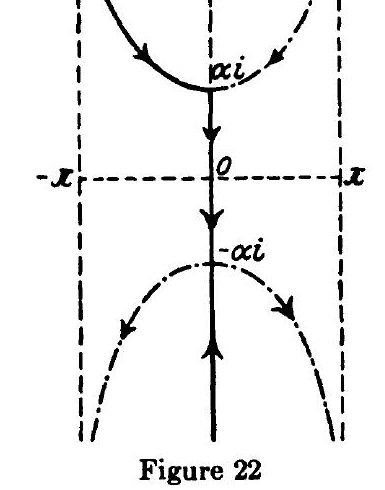
\includegraphics[width=0.30\textwidth]{figures/ch07_fig22.png}
\end{center}

% --- printed p.529 ---
\begin{align*}
\int_{(-\alpha-\epsilon)i}^{(-\alpha+\epsilon)i}e^{\lambda f(\tau)}\,d\tau
&=e^{\lambda(\alpha-\tanh\alpha)}
\int_{(-\alpha-\epsilon)i}^{(-\alpha+\epsilon)i}
 e^{\lambda\tanh\alpha(\tau+\alpha i)^2/2}\,d\tau
\bigl(1+O(\lambda^{-1/5})\bigr)\\
&=i\sqrt{\frac{2}{\lambda\tanh\alpha}}e^{\lambda(\alpha-\tanh\alpha)}
\int_{-\epsilon\sqrt{\lambda\tanh\alpha/2}}^{+\epsilon\sqrt{\lambda\tanh\alpha/2}}e^{-u^2}\,du
\bigl(1+O(\lambda^{-1/5})\bigr)\\
&=i\sqrt{\frac{2}{\lambda\tanh\alpha}}e^{\lambda(\alpha-\tanh\alpha)}
\int_{-\infty}^{\infty}e^{-u^2}\,du
\bigl(1+O(e^{-c_3\lambda\epsilon^2})\bigr)
\bigl(1+O(\lambda^{-1/5})\bigr)\\
&=i\sqrt{\frac{2\pi}{\lambda\tanh\alpha}}e^{\lambda(\alpha-\tanh\alpha)}
\bigl(1+O(e^{-c_3\lambda\epsilon^2})\bigr)
\bigl(1+O(\lambda^{-1/5})\bigr).
\end{align*}

\begin{center}
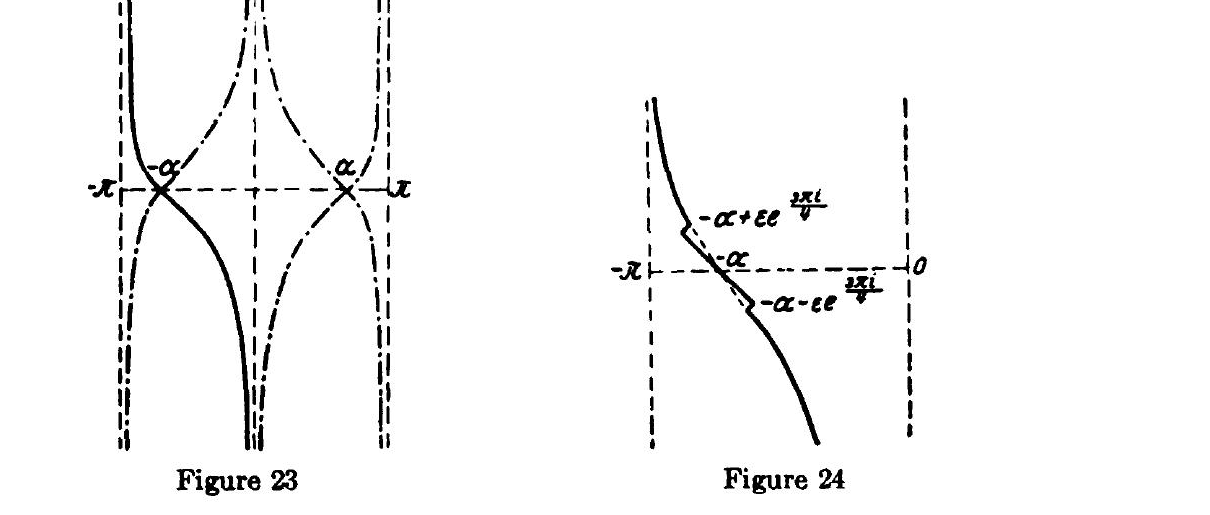
\includegraphics[width=0.70\textwidth]{figures/ch07_fig23_24.png}
\end{center}

Thus we have
\begin{equation}\tag{93}
H_\lambda^1(a\lambda)=-i\sqrt{\frac{2}{\pi\lambda\tanh\alpha}}
 e^{\lambda(\alpha-\tanh\alpha)}\bigl(1+O(\lambda^{-1/5})\bigr).
\end{equation}

(2) If $a>1$, say $a=1/\cos\alpha$ $(0<\alpha<\pi/2)$, we have the saddle points $\tau=\pm\alpha$ and the curves
\[
u-a\sin u\cosh v=\pm(\alpha-a\sin\alpha),
\qquad
\cosh v=\frac{u\mp(\alpha-\tan\alpha)}{a\sin u},
\]
which are reproduced in Figure 23; the solid path represents $H_\lambda^1(x)$. In the neighborhood of the saddle point, we replace this path by a line-segment making an angle $-\pi/4$ with the real axis, and by connecting segments of bounded length on which $\Im f(\tau)$ does not assume values larger than its value at the points $\tau=-\alpha\pm\epsilon e^{3\pi i/4}$ (see Figure 24). Again we set $\epsilon=\lambda^{-2/5}$, and obtain as before

% --- printed p.530 ---
\begin{align*}
\int_{L_1'} e^{\lambda f(\tau)}\,d\tau
&=e^{\lambda f(-\alpha)}
\int_{-\alpha-\epsilon e^{3\pi i/4}}^{-\alpha+\epsilon e^{3\pi i/4}}
 e^{(\lambda/2)f''(-\alpha)(\tau+\alpha)^2}\,d\tau
 \bigl(1+O(\lambda^{-1/5})\bigr)\\
&=e^{i\lambda(\tan\alpha-\alpha)}
\int_{-\alpha-\epsilon e^{3\pi i/4}}^{-\alpha+\epsilon e^{3\pi i/4}}
 e^{-(\lambda i/2)\tan\alpha\,(\tau+\alpha)^2}\,d\tau
 \bigl(1+O(\lambda^{-1/5})\bigr)\\
&=e^{3\pi i/4}\sqrt{\frac{2}{\lambda\tan\alpha}}\,
 e^{i\lambda(\tan\alpha-\alpha)}
\int_{-\epsilon\sqrt{\lambda\tan\alpha/2}}^{+\epsilon\sqrt{\lambda\tan\alpha/2}}
 e^{-u^2}\,du\bigl(1+O(\lambda^{-1/5})\bigr)\\
&=e^{3\pi i/4}\sqrt{\frac{2\pi}{\lambda\tan\alpha}}\,
 e^{i\lambda(\tan\alpha-\alpha)}
 \bigl(1+O(e^{-c_3\lambda\epsilon^2})\bigr)
 \bigl(1+O(\lambda^{-1/5})\bigr),
\end{align*}
whence
\begin{equation}\tag{94}
H_\lambda^1(a\lambda)
=-e^{3\pi i/4}\sqrt{\frac{2}{\pi\lambda\tan\alpha}}\,
 e^{i\lambda(\tan\alpha-\alpha)}\bigl(1+O(\lambda^{-1/5})\bigr).
\end{equation}

\begin{center}
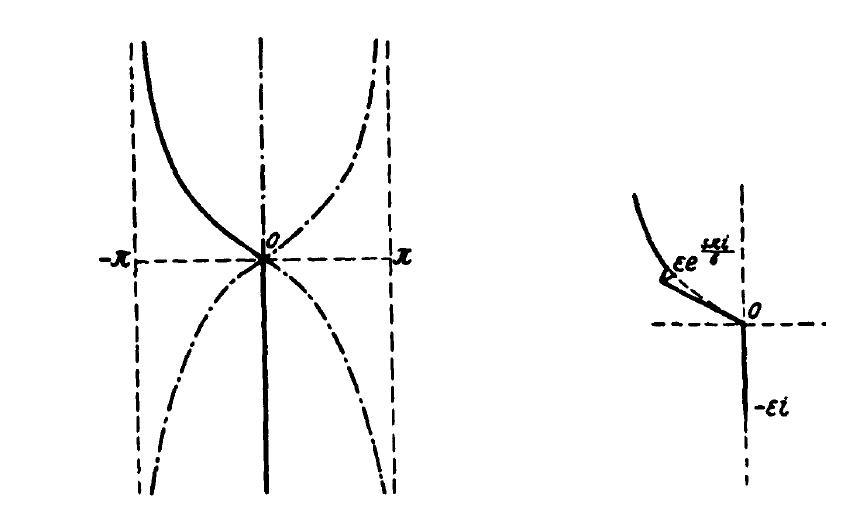
\includegraphics[width=0.58\textwidth]{figures/ch07_fig25_26.png}
\end{center}

(3) If $a=1$, $f''(\tau)$ also vanishes at the saddle point $\tau=0$ and the
curve $\Im f(\tau)=u-\sin u\cosh v=\Im f(0)=0$ has three branches
through $\tau=0$ (Figure 25), one of which is the imaginary axis. Again
we replace the curved part of the path $L_1$ (Figure 25) which is close
to $\tau=0$ by a straight segment of length $\epsilon=\lambda^{-1/4}$ inclined at the
angle $5\pi/6$ with the real axis (see Figure 26) and obtain for all $\tau$ of
the path of integration between $-\epsilon i$ and $\epsilon e^{5\pi i/6}$
\[
\left|f(\tau)-\frac{i\tau^3}{6}\right|\le c_1\epsilon^5.
\]
Moreover, we have
\[
\int_{L_1}e^{\lambda f(\tau)}\,d\tau
=\int_{-\epsilon i}^{\epsilon e^{5\pi i/6}}e^{\lambda f(\tau)}\,d\tau
+O(e^{-c_1\lambda\epsilon^3}),
\]

% --- printed p.531 ---
\[
\int_{-\epsilon i}^{\epsilon e^{5\pi i/6}}e^{\lambda f(\tau)}\,d\tau
=\int_{-\epsilon i}^{\epsilon e^{5\pi i/6}}e^{\lambda i\tau^3/6}\,d\tau
\bigl(1+O(\lambda^{-1/4})\bigr),
\]
\[
\int_{-\epsilon i}^{\epsilon e^{5\pi i/6}}e^{\lambda i\tau^3/6}\,d\tau
=\left(\int_0^{\epsilon e^{5\pi i/6}}-\int_0^{-\epsilon i}\right)e^{\lambda i\tau^3/6}\,d\tau
=\sqrt[3]{\frac6\lambda}\,(e^{5\pi i/6}+i)
\int_0^{\epsilon\sqrt[3]{\lambda/6}}e^{-u^3}\,du;
\]
in the last transformation we use the substitution
$\tau=\sqrt[3]{6/\lambda}\,e^{5\pi i/6}u$ in the first integral and
$\tau=-\sqrt[3]{6/\lambda}\,iu$ in the second. The right side of the last equation equals
\[
\sqrt[3]{\frac6\lambda}\,(e^{5\pi i/6}+i)
\int_0^\infty e^{-u^3}\,du\bigl(1+O(e^{-c_3\epsilon^3\lambda})\bigr),
\]
if $\epsilon^3\lambda$ remains greater than a positive bound. On the other hand we have
\[
\int_0^\infty e^{-u^3}\,du
=\frac13\int_0^\infty e^{-t}t^{-2/3}\,dt
=\frac13\Gamma\!\left(\frac13\right)
\]
and, therefore, finally
\begin{equation}\tag{95}
H_\lambda^1(\lambda)
=-\frac1{3\pi}\Gamma\!\left(\frac13\right)
(e^{5\pi i/6}+i)\sqrt[3]{\frac6\lambda}\,
\bigl(1+O(\lambda^{-1/4})\bigr).
\end{equation}

To find asymptotic formulas for $J_\lambda(a\lambda)$ in the cases $a\ge1$ we use
the formulas derived above for $H_\lambda^1(a\lambda)$ and the following three formulas which are found in a similar way:
\begin{equation}\tag{96}
H_\lambda^2(a\lambda)
=i\sqrt{\frac{2}{\pi\lambda\tanh\alpha}}\,
 e^{\lambda(\alpha-\tanh\alpha)}\bigl(1+O(\lambda^{-1/5})\bigr)
\qquad(a<1),
\end{equation}
\begin{equation}\tag{96'}
H_\lambda^2(a\lambda)
=-e^{-3\pi i/4}\sqrt{\frac{2}{\pi\lambda\tan\alpha}}\,
 e^{-i\lambda(\tan\alpha-\alpha)}\bigl(1+O(\lambda^{-1/5})\bigr)
\qquad(a>1),
\end{equation}
\begin{equation}\tag{96''}
H_\lambda^2(\lambda)
=-\frac1{3\pi}\Gamma\!\left(\frac13\right)(e^{-5\pi i/6}-i)
\sqrt[3]{\frac6\lambda}\,\bigl(1+O(\lambda^{-1/4})\bigr)
\qquad(a=1).
\end{equation}
We combine them by means of
\[
J_\lambda(x)=\tfrac12\bigl(H_\lambda^1(x)+H_\lambda^2(x)\bigr);
\]
the principal term turns out to be zero only in the case $a<1$. In this case we can take the path shown in Figure 27 for $J_\lambda$ also, obtaining by the same method

% --- printed p.532 ---
\[
J_\lambda(a\lambda)
=\frac{2}{\sqrt{2\pi\lambda\tanh\alpha}}\,
 e^{\lambda(\tanh\alpha-\alpha)}\bigl(1+O(\lambda^{-1/5})\bigr).
\]

\subsection{General Remarks on the Saddle Point Method}
Here the saddle point method has been used only to derive asymptotic formulas for the first terms of asymptotic series found as originally indicated. The reader is referred to the detailed presentation of these series in G. N. Watson, \emph{A Treatise on the Theory of Bessel Functions}, Cambridge University Press, Cambridge, 1922, and to the literature, in particular P. Debye, N\"aherungsformeln f\"ur die Zylinderfunktionen f\"ur grosse Werte des Arguments und unbeschr\"ankt ver\"anderliche Werte des Index, \emph{Math. Ann.}, Vol. 67, 1909, pp. 535--558.

\begin{center}
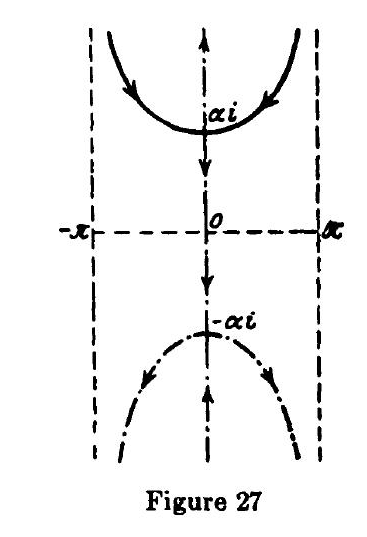
\includegraphics[width=0.24\textwidth]{figures/ch07_fig27.png}
\end{center}

In applications of the saddle point method it is not necessary to take the path of integration precisely in the manner described. It is enough if eventually, i.e. for large values of the parameter in terms of which the functions are expanded, the path comes sufficiently close to the one described. In this way Faber\footnote{G. Faber, Absch\"atzung von Funktionen grosser Zahlen, S.-Ber. Akad. M\"unchen (math.-phys. Kl.), 1922, pp. 285--304.} obtains a number of asymptotic series, e.g. for Hermite and Laguerre polynomials.

\subsection{The Darboux Method}
A different method for deriving asymptotic formulas is due to Darboux.\footnote{G. Darboux, M\'emoire sur l'approximation des fonctions de tr\`es-grands nombres, et sur une classe \'etendue de d\'eveloppements en s\'erie, J. de math. pures et appl., Ser. 3, Vol. 4, 1878, pp. 5--56 and 377--416. See also A. Haar, \"Uber asymptotische Entwicklungen von Funktionen, Math. Ann., Vol. 96, 1926, pp. 69--107.}
Let the quantities $a_\nu$ in question be given as the coefficients of a power series, hence by a generating function
$K(\zeta)=\sum_{\nu=0}^\infty a_\nu\zeta^\nu$. If we know the singularities of this function on the circle of convergence---say $|\zeta|=1$, $\zeta=e^{i\varphi}$---and if by subtracting known functions
$f_n(\zeta)=\sum_{\nu=0}^\infty \alpha_{n\nu}\zeta^\nu$ we can insure that the remainder $K-f_n$ converges uniformly, as we approach the circle of convergence, to an $n$-times continuously differentiable function

% --- printed p.533 ---
of $\varphi$, then the coefficients $a_\nu-\alpha_{n\nu}$ of the power series
\[
K(\zeta)-f_n(\zeta)=\sum_{\nu=0}^\infty(a_\nu-\alpha_{n\nu})\zeta^\nu
\]
are the Fourier coefficients of an $n$-times continuously differentiable (i.e. for $n=0$, just continuous) function of $\varphi$; hence, by Ch. II, \S5, 3, they satisfy the condition
\[
\lim_{\nu\to\infty}\nu^{n-1}|a_\nu-\alpha_{n\nu}|=0.
\]
Thus if $\nu$ is large, the approximation of $a_\nu$ by $\alpha_{n\nu}$ becomes better as $n$ increases.

\subsection{Application of the Darboux Method to the Asymptotic Expansion of Legendre Polynomials}
We apply the method to the Legendre polynomials $P_\nu(x)$ which are given by means of the generating function
\begin{equation}\tag{97}
K(z,\zeta)=\frac1{\sqrt{1-2z\zeta+\zeta^2}}
=\sum_{\nu=0}^\infty P_\nu(z)\zeta^\nu.
\end{equation}
Assume $-1<z<1$, $z=\cos\varphi$, $0<\varphi<\pi$. Then
$1-2z\zeta+\zeta^2=(\zeta-e^{\varphi i})(\zeta-e^{-\varphi i})$; the circle of convergence has radius 1, and on it lie the singular points $\zeta=e^{\pm\varphi i}$. In order to derive the series expansion of $K$ according to powers of $\zeta-e^{\pm\varphi i}$, we make the convention that
\[
\sqrt{\zeta-e^{\pm\varphi i}}
=e^{\pm i(\varphi+\pi)/2}\sqrt{1-\zeta e^{\mp\varphi i}},
\]
where the square root on the right denotes the branch presented by the binomial series.\footnote{Thus if $a$ is a positive number, for $\zeta=e^{\varphi i}-a$ the root $\sqrt{\zeta-e^{\varphi i}}$ is positive imaginary, while for $\zeta=e^{-\varphi i}-a$ the root $\sqrt{\zeta-e^{-\varphi i}}$ is negative imaginary. The above convention is in agreement with the requirement, which follows from formula (97), that for $\zeta=0$ the root $\sqrt{1-2z\zeta+\zeta^2}$ should take the value $+1$.}
We obtain
\begin{align*}
K(z,\zeta)
&=\frac1{\sqrt{\zeta-e^{\varphi i}}}
 \bigl[(\zeta-e^{\varphi i})+(e^{\varphi i}-e^{-\varphi i})\bigr]^{-1/2}\\
&=\frac{e^{3\pi i/4}}{\sqrt{2\sin\varphi}}\,
 \frac1{\sqrt{\zeta-e^{\varphi i}}}
 \sum_{\nu=0}^\infty\binom{-\tfrac12}{\nu}
 \left(\frac{\zeta-e^{\varphi i}}{e^{\varphi i}-e^{-\varphi i}}\right)^\nu\\
&=\frac{e^{-3\pi i/4}}{\sqrt{2\sin\varphi}}\,
 \frac1{\sqrt{\zeta-e^{-\varphi i}}}
 \sum_{\nu=0}^\infty\binom{-\tfrac12}{\nu}
 \left(\frac{\zeta-e^{-\varphi i}}{e^{-\varphi i}-e^{\varphi i}}\right)^\nu.
\end{align*}

% --- printed p.534 ---
If we set
\[
\begin{aligned}
f_n(z,\zeta)=\frac1{\sqrt{2\sin\varphi}}\sum_{\nu=0}^n\binom{-\tfrac12}{\nu}
\Biggl\{&e^{3\pi i/4}\frac{(\zeta-e^{\varphi i})^{\nu-1/2}}{(e^{\varphi i}-e^{-\varphi i})^\nu}\\
&+e^{-3\pi i/4}\frac{(\zeta-e^{-\varphi i})^{\nu-1/2}}{(e^{-\varphi i}-e^{\varphi i})^\nu}\Biggr\},
\end{aligned}
\]
then $K-f_n$ is $n$-times continuously differentiable on the circle of convergence. Hence if we expand $f_n$ in powers of $\zeta$ and, for convenience, write
$(3\pi/4)+(\varphi+\pi)(\nu-\tfrac12)=\omega$, we obtain
\begin{align*}
f_n(z,\zeta)
&=\frac1{\sqrt{2\sin\varphi}}\sum_{\nu=0}^n\binom{-\tfrac12}{\nu}
\left\{\frac{e^{i\omega}(1-\zeta e^{-\varphi i})^{\nu-1/2}}{(e^{\varphi i}-e^{-\varphi i})^\nu}
+\frac{e^{-i\omega}(1-\zeta e^{\varphi i})^{\nu-1/2}}{(e^{-\varphi i}-e^{\varphi i})^\nu}\right\}\\
&=\frac1{\sqrt{2\sin\varphi}}\sum_{\nu=0}^n\binom{-\tfrac12}{\nu}
\sum_{\mu=0}^\infty\binom{\nu-\tfrac12}{\mu}\zeta^\mu
\left\{\frac{e^{i[\omega-(\varphi+\pi)\mu]}}{(e^{\varphi i}-e^{-\varphi i})^\nu}
+\frac{e^{-i[\omega-(\varphi+\pi)\mu]}}{(e^{-\varphi i}-e^{\varphi i})^\nu}\right\}\\
&=\sum_{\mu=0}^\infty p_{n\mu}(z)\zeta^\mu
\end{align*}
with
\[
\begin{aligned}
p_{n\mu}=\frac1{\sqrt{2\sin\varphi}}\sum_{\nu=0}^n
\binom{-\tfrac12}{\nu}\binom{\nu-\tfrac12}{\mu}\frac1{(2\sin\varphi)^\nu}
\Bigl[&e^{i[\pi/4+(\nu-\mu-1/2)\varphi-(\mu-\nu/2)\pi]}\\
&+e^{-i[\pi/4+(\nu-\mu-1/2)\varphi-(\mu-\nu/2)\pi]}\Bigr],
\end{aligned}
\]
that is,
\begin{equation}\tag{98}
\begin{aligned}
p_{n\mu}=\frac{2}{\sqrt{2\sin\varphi}}\sum_{\nu=0}^n
\binom{-\tfrac12}{\nu}\binom{\nu-\tfrac12}{\mu}
\frac{(-1)^\mu}{(2\sin\varphi)^\nu}
\cos\left(\frac\pi4(1+2\nu)-(\nu-\mu-\tfrac12)\varphi\right).
\end{aligned}
\end{equation}
we obtain
\[
P_\mu(z)=p_{n,\mu}(z)+O(\mu^{-n})
\]
uniformly in every interval of the form $-1+\epsilon\le z\le1-\epsilon$ $(0<\epsilon<1)$. In view of the fact that $p_{n+1,\mu}-p_{n,\mu}=O(\mu^{-n-1})$, it follows that
\[
P_\mu(z)=p_{n,\mu}(z)+O(\mu^{-n-1}).
\]

% --- printed p.535 ---
The first term of this asymptotic expansion may be written as
\begin{equation}\tag{99}
P_\mu(z)=\frac{2}{\sqrt{2\sin\varphi}}
\frac{1\cdot3\cdots(2\mu-1)}{2\cdot4\cdots2\mu}
\cos\left(\frac\pi4-(\mu+\tfrac12)\varphi\right)+O\!\left(\frac1\mu\right).
\end{equation}
If $z$ is not real between $-1$ and $+1$, then since the singular points $\zeta_1,\zeta_2$ satisfy $\zeta_1\zeta_2=1$, one of them, say $\zeta_1$, has a modulus $|\zeta_1|<1$, the other a modulus $|\zeta_2|>1$. Only the singular point $\zeta_1$ lies on the circle of convergence $|\zeta|=|\zeta_1|$; hence we need consider only this singularity. Accordingly, if we transform the first $n$ terms of the expansion of $K(z,\zeta)$ in terms of powers of $\zeta-\zeta_1$ into a power series in $\zeta$, the coefficients provide asymptotic expressions for $P_\nu(z)$; however, now only
\[
|\zeta_1|^\nu(P_\nu-p_{n\nu})=O(\nu^{-n-1})
\]
holds.

\begin{center}
{\LARGE\bfseries\color{BellaInk} Appendix to Chapter VII}
\end{center}
\vspace{1em}

\section[Transformation of Spherical Harmonics]{Transformation of Spherical Harmonics\protect\footnotemark}
\footnotetext{The author is indebted to W. Magnus for this appendix, which is based on unpublished notes by the late G. Herglotz.}

\subsection{Introduction and Notation}
Let $x,y,z$ be Cartesian coordinates and let $r,\theta,\varphi$ be spherical polar coordinates defined by
\begin{equation}\tag{100}
x=r\cos\varphi\sin\theta,\qquad y=r\sin\varphi\sin\theta,\qquad z=r\cos\theta.
\end{equation}
Let $\Delta$ denote Laplace's operator
\begin{equation}\tag{101}
\begin{aligned}
\Delta&=\frac{\partial^2}{\partial x^2}+\frac{\partial^2}{\partial y^2}+\frac{\partial^2}{\partial z^2}\\
&=\frac{\partial^2}{\partial r^2}+\frac2r\frac{\partial}{\partial r}
+\frac1{r^2}\frac{\partial^2}{\partial\theta^2}
+\frac{\cot\theta}{r^2}\frac{\partial}{\partial\theta}
+\frac1{r^2\sin^2\theta}\frac{\partial^2}{\partial\varphi^2}.
\end{aligned}
\end{equation}
A function $u$ which satisfies $\Delta u=0$ is called harmonic. If $p_n(\theta,\varphi)$ is a one-valued function of $x,y,z$ such that $r^np_n$ is a harmonic function,

% --- printed p.536 ---
$p_n$ is called a spherical harmonic of order $n$. It was observed in \S5 that $r^np_n$ is a homogeneous harmonic polynomial of degree $n$ in $x,y,z$ and vice versa.

In several problems of mathematical physics the question arises how any set of linearly independent spherical harmonics is transformed if the coordinate system is rotated but the origin $r=0$ kept fixed. To answer this question, we shall characterize the orthogonal transformations in terms of independent parameters $q_\nu$ $(\nu=1,2,3,4)$. Coordinate rotation in a system of $2n+1$ linearly independent spherical harmonics of order $n$ is expressed by a linear substitution whose coefficients form a complete system of orthogonal hyperspherical harmonics of order $2n$ in the four-dimensional space of the parameters $q_\nu$.

There exists no analogue to this result in the case of more than three variables.

\subsection{Orthogonal Transformations}
Let $O$ be an orthogonal matrix of three rows and three columns; $O$ is characterized by
\begin{equation}\tag{102}
OO'=I
\end{equation}
where $O'$ is the transposed matrix of $O$ and $I$ denotes the identity or unit matrix. We shall consider only ``proper'' orthogonal matrices; i.e., we assume that the determinant $|O|$ of $O$ equals $+1$. Let
\begin{equation}\tag{103}
A=\begin{pmatrix}
0&q_3&-q_2\\
-q_3&0&q_1\\
q_2&-q_1&0
\end{pmatrix}
\end{equation}
be a skew-symmetric matrix, i.e. one for which $A'=-A$. Let $q_4$ be a fourth parameter and let
\begin{equation}\tag{104}
w=(q_1^2+q_2^2+q_3^2)^{1/2},\qquad
v=(q_1^2+q_2^2+q_3^2+q_4^2)^{1/2}.
\end{equation}
Then we have

\emph{Cayley's theorem: For any real values of the $q_\nu$ $(\nu=1,2,3,4)$ for which $v>0$, the matrix}
\begin{equation}\tag{105}
O=(q_4I+A)(q_4I-A)^{-1}
=\frac1{v^2}(v^2I+2q_4A+2A^2),
\end{equation}

% --- printed p.537 ---
or
\begin{equation}\tag{106}
O=\frac1{v^2}\begin{pmatrix}
q_4^2+q_1^2-q_2^2-q_3^2 & 2q_1q_2+2q_3q_4 & 2q_1q_3-2q_2q_4\\
2q_1q_2-2q_3q_4 & q_4^2+q_2^2-q_1^2-q_3^2 & 2q_2q_3+2q_1q_4\\
2q_1q_3+2q_2q_4 & 2q_2q_3-2q_1q_4 & q_4^2+q_3^2-q_1^2-q_2^2
\end{pmatrix},
\end{equation}
\emph{is orthogonal; $q_1/w$, $q_2/w$, $q_3/w$ are the direction cosines of the axis of rotation with respect to the $x$-, $y$-, and $z$-axes. If $\omega$ denotes the angle of rotation, then}
\begin{equation}\tag{107}
\cos\frac\omega2=\frac{q_4}{v},\qquad \sin\frac\omega2=\frac{w}{v}.
\end{equation}
\emph{We normalize the parameters $q_\nu$ in such a way that}
\begin{equation}\tag{108}
v^2=q_1^2+q_2^2+q_3^2+q_4^2=1
\end{equation}
\emph{holds; then any two sets $q_\nu$ and $q_\nu^*$ of values of the parameters define the same $O$ if and only if $q_\nu=q_\nu^*$ or $q_\nu=-q_\nu^*$ for $\nu=1,2,3,4$.} If $w=0$, every direction in the space remains fixed and $O$ becomes the identity $I$.

Proof: We say that two matrices $B$ and $C$ commute if $BC=CB$. We may then perform all algebraic operations as if $B$ and $C$ were numbers provided we do not divide by any matrix unless its determinant is different from zero; for instance, if $|B|\ne0$, $B^{-1}$ and $C$ also commute. Using this fact and the well-known relation $(B')^{-1}=(B^{-1})'$ (where the prime denotes a transposed matrix) we see at once: If $q_4I-A$ has an inverse and if, as in (105), we set
\begin{equation}\tag{109}
O=(q_4I+A)(q_4I-A)^{-1},
\end{equation}
then
\begin{equation}\tag{110}
O'=(q_4I'-A')^{-1}(q_4I'+A')=(q_4I-A)(q_4I+A)^{-1}=O^{-1}.
\end{equation}
Therefore $O$ is orthogonal. Similarly, we find for any orthogonal $O$ for which $|I+O|\ne0$ that
\begin{equation}\tag{111}
A=q_4(I-O)(I+O)^{-1}
\end{equation}
is a skew-symmetric matrix. But (111) is exactly the expression for $A$ which we obtain if we ``solve'' (109) with respect to $A$. This

% --- printed p.538 ---
proves the first part of Cayley's theorem (i.e. (105) and (106)) unless $|I+O|=0$. Even in this case, the right side in (109) has a meaning if we write it in a different form. Since every matrix satisfies its characteristic equation, we have
\begin{equation}\tag{112}
A^3+w^2A=0,
\end{equation}
which (for $v>0$) leads to
\begin{equation}\tag{113}
q_4I+A=v^{-2}(v^2I+2q_4A+2A^2)(q_4I-A).
\end{equation}
We may define the right side in (109) as $v^{-2}(v^2I+2q_4A+2A^2)$; then, however, we have to show that this is an orthogonal matrix even if $|q_4I-A|=0$, i.e. if $q_4$ is an eigenvalue of $A$. Since $A$ is skew-symmetric, its eigenvalues are pure imaginary. Hence $q_4=0$ and
\begin{equation}\tag{114}
v^{-2}(v^2I+2q_4A+2A^2)=I+2w^{-2}A^2;
\end{equation}
because of (112) we have
\begin{equation}\tag{115}
(I+2w^{-2}A^2)^2=I+4w^{-2}A^2+4w^{-4}A^4=I.
\end{equation}
Therefore, for $q_4=0$, $I+2w^{-2}A^2$ is a symmetric orthogonal matrix. It can be verified that all orthogonal matrices of this type can be written in the form $I+2w^{-2}A^2$. On the other hand, any orthogonal matrix for which $|O|=+1$ and $|I+O|=0$ is necessarily symmetric because such an $O$ must have the eigenvalues $+1,-1,-1$; its square has the eigenvalues $1,1,1$, and is therefore the identity. But $O^2=OO'=I$ implies that $O$ is symmetric.

In order to interpret the $q_\nu$ geometrically, we observe first that the vector $(q_1,q_2,q_3)$ is an eigenvector of $A$ belonging to the eigenvalue zero. It follows from (105) that $(q_1,q_2,q_3)$ is an eigenvector of $O$ belonging to the eigenvalue 1 and therefore defining the axis of rotation. Since the eigenvalues of $O$ are $\exp\{i\omega\}$, $\exp\{-i\omega\}$, and $1$, and since the sum of these is the trace of $O$, (107) follows from (106) except for the sign of $\cos(\omega/2)$, which need not be determined; for if we change $\omega/2$ by $\pi$, then $\omega$ changes by $2\pi$.

Apparently, Cayley's theorem can be extended to more than three dimensions, but then the explicit formulas (105) and (106) become more complicated. In three dimensions, (106) can be stated in a

% --- printed p.539 ---
simple manner by using quaternions.\footnote{Quaternions are ``hypercomplex'' numbers with three ``imaginary'' units $i,j,k$ which satisfy the relations $i^2=j^2=k^2=-1$, $ij=k$, $jk=i$, $ki=j$, $ij+ji=0$, $ik+ki=0$, $jk+kj=0$. The general quaternion is $a=a+bi+cj+dk$ where $a,b,c,d$ are real. All laws of algebra with the exception of the commutative law of multiplication are satisfied by quaternions.}
Let the vectors $\mathbf{x}$ and $\mathbf{x}'$ be defined by $\mathbf{x}=(x,y,z)$ and $\mathbf{x}'=O\mathbf{x}$. Let $\xi,\xi',\alpha$ be quaternions defined by
\begin{equation}\tag{116}
\xi=xi+yj+zk,\qquad \xi'=x'i+y'j+z'k
\end{equation}
and
\begin{equation}\tag{116'}
\alpha=-q_4+q_1i+q_2j+q_3k;
\end{equation}
then
\begin{equation}\tag{117}
\xi'=\alpha\xi\alpha^{-1}
\end{equation}
where $\alpha\alpha^{-1}=\alpha^{-1}\alpha=1$ and
$\alpha^{-1}=v^{-2}(-q_4-q_1i-q_2j-q_3k)$.

It may be observed that there exists a one-to-two correspondence between the elements of the orthogonal group and the points on a four-dimensional hypersphere. There also exists a group $G$ such that the orthogonal group is a quotient group of $G$ and the elements of $G$ are in a one-to-one correspondence with the points of the hypersphere. For a definition of this group see \S4; for its significance consult, e.g., B. L. van der Waerden, \emph{Die gruppentheoretische Methode in der Quantenmechanik}, \S16, J. Springer, Berlin, 1932.

\subsection{A Generating Function for Spherical Harmonics}
Let $P_{n,l}(x)$ denote the functions defined in Ch. VII, \S5, 1 for $l=0,1,2,\ldots,n$ and let
\begin{equation}\tag{118}
P_{n,-l}(x)=(-1)^l\frac{(n-l)!}{(n+l)!}P_{n,l}(x).
\end{equation}
Then we know that the $2n+1$ functions
\begin{equation}\tag{119}
P_{n,l}(\cos\theta)e^{il\varphi}\qquad(l=0,\pm1,\pm2,\ldots,\pm n)
\end{equation}

% --- printed p.540 ---
form a complete set of linearly independent spherical harmonics of order $n$. We assert that:

\emph{The homogeneous polynomials $h_{n,l}$ of degree $n$ in $x,y,z$ which are defined by}
\begin{equation}\tag{120}
\{x-iy-2zt-(x+iy)t^2\}^n
=t^n\sum_{l=-n}^{+n}h_{n,l}(x,y,z)t^l
\end{equation}
\emph{form a complete system of linearly independent harmonic polynomials of degree $n$. If spherical polar coordinates are introduced by equation (100), we have}
\begin{equation}\tag{121}
h_{n,l}(x,y,z)=r^np_{n,l}(\theta,\varphi)
\end{equation}
\emph{where}
\begin{equation}\tag{122}
p_{n,l}(\theta,\varphi)=(-1)^n\frac{2^nn!}{(n+l)!}P_{n,l}(\cos\theta)e^{il\varphi}.
\end{equation}
\emph{If $x,y,z$ are connected by a relation}
\begin{equation}\tag{123}
x^2+y^2+z^2=0,
\end{equation}
\emph{then $h_{n,l}$ can be expressed in terms of two parameters $w_1,w_2$ by}
\begin{equation}\tag{124}
h_{n,l}(x,y,z)=(-1)^n\binom{2n}{n+l}w_1^{n+l}w_2^{n-l}
\end{equation}
\emph{where}
\begin{equation}\tag{125}
x+iy=w_1^2,\qquad -x+iy=w_2^2,\qquad z=w_1w_2.
\end{equation}

Proof: If $a,b,c$ are any three numbers which satisfy $a^2+b^2+c^2=0$, then clearly $\Delta(ax+by+cz)^n=0$ holds; substituting $a=1-t^2$, $b=-i(1+t^2)$, $c=-2t$, we obtain (120). In order to prove equations (121) and (122) we substitute $t^{-1}$ for $t$ in (120) and find
\begin{equation}\tag{126}
h_{n,-l}=(-1)^l\overline{h_{n,l}}
\end{equation}
where the bar denotes a conjugate complex quantity. Therefore it suffices to prove (122) for $l\ge0$. Introducing $t=e^{-i\varphi}s$ in (120), we find
\begin{equation}\tag{127}
\{(1-s^2)\sin\theta-2s\cos\theta\}^n
=s^n\sum_{l=-n}^{+n}p_{n,l}(\theta,\varphi)e^{-il\varphi}s^l
\end{equation}

% --- printed p.541 ---
and see that
\[
p_{n,l}e^{-il\varphi}=f_{n,l}(\theta)
\]
is a real function of $\theta$ only. From (126) we obtain
\begin{equation}\tag{128}
f_{n,-l}(\theta)=(-1)^lf_{n,l}(\theta).
\end{equation}
If we multiply (127) by $s^{-n}$, substitute $\exp\{i(\omega+\pi/2)\}$ for $s$, and use (128), we obtain
\begin{equation}\tag{129}
(\cos\theta+i\cos\omega\sin\theta)^n
=(-2)^{-n}\left\{f_{n,0}+2\sum_{l=1}^n i^lf_{n,l}\cos l\omega\right\}.
\end{equation}
On the other hand, the integral representations for $P_{n,l}(x)$ with $l=0,1,2,\ldots,n$ (see \S4, 4) show that
\[
a_l=\frac{i^l}{(n+l)!}P_{n,l}(x)
\]
is the Fourier coefficient in the expansion of
\begin{equation}\tag{130}
(x+i\sqrt{1-x^2}\cos\omega)^n=a_0+2\sum_{l=1}^na_l\cos l\omega.
\end{equation}
Setting $x=\cos\theta$ and comparing equations (130) and (129), we see that (122) holds.

Finally, (124) becomes a trivial application of the binomial theorem if in (120) we substitute the expressions for $x,y,z$ given by (125).

It should be emphasized that equation (123) is not only a consequence of (125), but that any three numbers $x,y,z$ satisfying (123) define exactly two pairs of numbers $w_1,w_2$ such that equations (125) hold. Since $x+iy$ and $x-iy$ are algebraically independent, the polynomials in $w_1,w_2$ on the right side of (124) are linearly independent. Therefore, (125) maps the harmonic polynomials $h_{n,l}$ on the linearly independent polynomials (of even degree) in $w_1$ and $w_2$. This also shows that every harmonic polynomial can be characterized by exactly one polynomial in three variables the sum of the squares of which is zero. Earlier in this chapter, the same fact was established by showing that the harmonic polynomials can be obtained if we apply a polynomial in the differential operators $\partial/\partial x$, $\partial/\partial y$, $\partial/\partial z$ to $r^{-1}=(x^2+y^2+z^2)^{-1/2}$, where the sum of the squares of these operators (if applied to $r^{-1}$) is evidently zero.

% --- printed p.542 ---
\subsection{Transformation Formula}
The significance of the formulas (120) to (125) will become clear when we have shown that any orthogonal transformation of $x,y,z$ can be obtained from a linear substitution of $w_1$ and $w_2$. This expresses the well-known fact that the real orthogonal group in three variables has a representation by (complex) two-by-two matrices.

Lemma: Let $w_1,w_2,x,y,z$ be connected by (125) and assume that
\begin{equation}\tag{131}
w_1'=\alpha w_1+\beta w_2,\qquad
w_2'=-\overline\beta w_1+\overline\alpha w_2
\end{equation}
and
\begin{equation}\tag{132}
x'+iy'=w_1'^2,\qquad -x'+iy'=w_2'^2,\qquad z'=w_1'w_2'.
\end{equation}
Then (125), (131), (132) define a linear substitution $M$ by which the vector $\mathbf{x}=(x,y,z)$ is mapped on $\mathbf{x}'=(x',y',z')=M\mathbf{x}$. If we choose
\begin{equation}\tag{133}
\alpha=(q_4-iq_3)/v,\qquad \beta=(-q_2+iq_1)/v,
\end{equation}
then $M$ is the matrix $O$ defined by (106).

The proof is trivial. If we replace $\alpha,\beta$ by $-\alpha,-\beta$ we obtain the same matrix $M=O$ as before. This shows that there are (at least) two different substitutions (131) which lead to the same orthogonal substitution $O$. As a matter of fact, there are exactly two such substitutions (131)\ctnote{The supplied scan refers here to substitutions (132); the substitutions just discussed are those defined in (131).}, and the group of these is the group $G$ mentioned at the end of subsection 2 of this Appendix.

We may use this lemma to prove the following theorem which in its present form is due to G. Herglotz:

\emph{Let $\mathbf{x}=(x,y,z)$ be transformed into $\mathbf{x}'=(x',y',z')$ by the orthogonal transformation $O$ defined by (105), (106). Then the spherical harmonics $h_{n,l}(x',y',z')$ can be expressed in terms of the $h_{n,r}(x,y,z)$ (which are defined by (120)) by}
\begin{equation}\tag{134}
h_{n,l}(x',y',z')
=\sum_{r=-n}^{n}
\frac{\binom{2n}{l+n}}{\binom{2n}{r+n}}
 v^{-2n}H_{2n}^{(n+l,n+r)}(q_\mu)h_{n,r}(x,y,z)
\end{equation}
\emph{where the $H_{2n}^{(n+l,n+r)}$ are homogeneous polynomials of degree $2n$ in the variables $q_\mu$ $(\mu=1,2,3,4)$ which satisfy}
\begin{equation}\tag{135}
\sum_{\mu=1}^4\frac{\partial^2}{\partial q_\mu^2}H_{2n}^{(n+l,n+r)}(q_\mu)=0
\end{equation}

% --- printed p.543 ---
\emph{and can be defined in terms of the generating function}
\begin{equation}\tag{136}
G_{2n}(q_\mu;s,t)
\equiv\{iq_3(1-st)+iq_1(s+t)+q_2(s-t)+q_4(1+st)\}^{2n}
\end{equation}
\emph{by}
\begin{equation}\tag{137}
G_{2n}(q_\mu;s,t)=\sum_{j,k=0}^{2n}\binom{2n}{j}H_{2n}^{(j,k)}(q_\mu)t^js^k.
\end{equation}
Explicit expressions for the $H_{2n}^{(r,l)}$ and a modified form of equation (135) (in polar coordinates) will be given in subsection 5.

Equation (135) can be deduced from (136) in the same way that the statement $\Delta h_{n,l}=0$ was deduced from (120). To prove equations (134) and (136) we use (124) and consider the effect of the linear transformation (131) upon the $h_{n,l}$. From equation (124) and equations (133) and (131) we find
\begin{equation}\tag{138}
h_{n,l}(x',y',z')=(-1)^n\binom{2n}{n+l}w_1'^{n+l}w_2'^{n-l},
\end{equation}
\begin{equation}\tag{139}
\begin{aligned}
h_{n,l}(x',y',z')
&=(-1)^n\left(\frac{w_2}{v}\right)^{2n}\binom{2n}{n+l}\\
&\quad\times\{-q_2+iq_1+(q_4-iq_3)s\}^{n+l}
\{q_4+iq_3+(q_2+iq_1)s\}^{n-l},
\end{aligned}
\end{equation}
where $s=w_1/w_2$. On the other hand, the right side in equation (136) is
\[
\{[q_4+iq_3+(iq_1+q_2)s]+[iq_1-q_2+(q_4-iq_3)s]t\}^{2n};
\]
therefore, the coefficient of $(-1)^n(w_2/v)^{2n}$ in (139) is precisely the coefficient of $t^{n+l}$ in (137) with $s=w_1/w_2$. We obtain
\begin{equation}\tag{140}
h_{n,l}(x',y',z')=(-1)^n\binom{2n}{n+l}v^{-2n}
\sum_{k=0}^{2n}H_{2n}^{(n+l,k)}w_1^kw_2^{2n-k},
\end{equation}
which together with (124) proves equation (134).

\subsection{Expressions in Terms of Angular Coordinates}
In polar coordinates the standard spherical harmonics express themselves in terms of $r,\theta,\varphi$ as products of functions of a single variable; however, the transformation formulas become simple in Cartesian coordinates. Indeed, if we set
\begin{equation}\tag{141}
x'=r'\cos\varphi'\sin\theta',\qquad
y'=r'\sin\varphi'\sin\theta',\qquad
z'=r'\cos\theta',
\end{equation}
\ctnote{In (141), the supplied scan prints $z'=\cos\theta'$. Consistency with the spherical-coordinate definition (100), and with the immediately following statement $r'=r$, requires the factor $r'$.}

% --- printed p.544 ---
we have $r'=r$, but $\theta',\varphi'$ cannot be expressed in a simple manner in terms of $\theta$ and $\varphi$. Nevertheless, the spherical harmonics
\[
(r')^{-n}h_{n,l}(x',y',z')=(-1)^n\frac{2^nn!}{(n+l)!}P_{n,l}(\cos\theta')e^{il\varphi'}
\]
can be expressed in terms of the $P_{n,l}(\cos\theta)\exp\{il\varphi\}$ if we use (134). Only the problem of finding simple explicit expressions for the $H_{2n}^{(n+l,n+r)}(q_\mu)$ remains. If we were to introduce four-dimensional (hyperspherical) polar coordinates in the space of the variables $q_\mu$, we would still obtain rather complicated formulas; however, there exists a particular coordinate system in which the expressions for the $H_{2n}^{(n+l,n+r)}$ become fairly simple. We may summarize the results as follows:

\emph{Let $v\ge0$, $0\le\rho\le2\pi$, $0\le\sigma\le2\pi$, $0\le\tau\le\pi/2$ and}
\begin{equation}\tag{142}
q_1=-v\sin\sigma\sin\tau,\qquad q_2=v\cos\sigma\sin\tau,
\qquad q_3=v\sin\rho\cos\tau,\qquad q_4=v\cos\rho\cos\tau.
\end{equation}
\emph{Then $v,\rho,\sigma,\tau$ are orthogonal coordinates; the line element is}
\begin{equation}\tag{143}
dq_1^2+dq_2^2+dq_3^2+dq_4^2
=dv^2+v^2\{\cos^2\tau\,d\rho^2+\sin^2\tau\,d\sigma^2+d\tau^2\}
\end{equation}
\emph{and the surface element of the hypersphere $\Omega$ (defined by $v=1$) is}
\begin{equation}\tag{144}
d\Omega=\cos\tau\sin\tau\,d\rho\,d\sigma\,d\tau.
\end{equation}
\emph{In these coordinates}
\begin{equation}\tag{145}
\begin{aligned}
v^{-2n}H_{2n}^{(n+l,n+r)}(q_\mu)
&=S_{2n}^{(l,r)}(\rho,\sigma,\tau)\\
&=\frac1{(n+r)!}e^{-i(l+r)\rho}e^{-i(r-l)\sigma}
(\cos\tau)^{l+r}(\sin\tau)^{r-l}F_{2n}^{(l,r)}(\cos^2\tau)
\end{aligned}
\end{equation}
\emph{where}
\begin{equation}\tag{146}
F_{2n}^{(l,r)}(t)=\frac{d^{n+r}}{dt^{n+r}}t^{n-l}(t-1)^{n+l}.
\end{equation}
\emph{The $S_{2n}^{(l,r)}$ and their conjugate complex functions are biorthogonal on the unit-hypersphere $\Omega$:}
\begin{equation}\tag{147}
\iiint_\Omega S_{2n}^{(l',r')}\,\overline{S_{2n}^{(l,r)}}\,d\Omega
=\begin{cases}
0,&l'\ne l\text{ or }r'\ne r,\\[4pt]
\displaystyle \frac{2\pi^2}{2n+1}\frac{\binom{2n}{r+n}}{\binom{2n}{l+n}},&l'=l\text{ and }r'=r.
\end{cases}
\end{equation}

% --- printed p.545 ---
\emph{The transformation formulas of the spherical harmonics are}
\begin{equation}\tag{148}
P_{n,l}(\cos\theta')e^{il\varphi'}
=\sum_{r=-n}^{n}\frac{(n-r)!}{(n-l)!}S_{2n}^{(l,r)}
P_{n,r}(\cos\theta)e^{ir\varphi}.
\end{equation}
Proof: If in (136) and (137) we substitute the expressions (142) for the $q_\nu$ and introduce $s^*$ and $t^*$ by
\[
s^*=se^{-i(\sigma+\rho)},\qquad t^*=te^{-i(\sigma-\rho)}
\]
we find, for the $S_{2n}^{(l,r)}$ in (145),
\begin{equation}\tag{149}
\begin{aligned}
\{(1+s^*t^*)\cos\tau+(s^*-t^*)\sin\tau\}^{2n}
=\sum_{l,r=-n}^{n}\binom{2n}{n+l}S_{2n}^{(l,r)}
 e^{i(r+l)\rho}e^{i(r-l)\sigma}(t^*)^{n+l}(s^*)^{n+r}.
\end{aligned}
\end{equation}
which proves that $S_{2n}^{(l,r)}\exp\{i[(r+l)\rho+(r-l)\sigma]\}=U_{2n}^{(l,r)}$ depends only on $\tau$. Comparing the coefficients of $(t^*)^{n+l}$ on both sides of (149), we find
\begin{equation}\tag{150}
\begin{aligned}
\sum_{r=-n}^{+n}U_{2n}^{(l,r)}(s^*)^{n+r}
&=(\cos\tau+s^*\sin\tau)^{n-l}(-\sin\tau+s^*\cos\tau)^{n+l}\\
&=(\cos\tau)^{l-n}(\sin\tau)^{-n-l}
[\cos^2\tau+s^*\cos\tau\sin\tau]^{n-l}\\
&\qquad\times[\cos^2\tau-1+s^*\cos\tau\sin\tau]^{n+l}.
\end{aligned}
\end{equation}
Application of Taylor's formula to the last line in (150) yields equations (145) and (146). From these formulas and from (144) we can derive (147) by repeated integration by parts if we observe that
\[
\overline{S_{2n}^{(l,r)}}=(-1)^{l+r}S_{2n}^{(-l,-r)}.
\]
We mention without proof that, according to a formula which was discovered by Jacobi, the $U_{2n}^{(l,r)}$ can also be expressed in terms of hypergeometric series (see Chapter II, equation (24) on page 90). These series are, for $l+r\le0$,
\[
U_{2n}^{(l,r)}=(-1)^{n+l}\binom{n-l}{n+r}
(\cos\tau)^{-l-r}(\sin\tau)^{l-r}
\,{}_2F_1(-n-r,n+1-r;1-l-r;\cos^2\tau),
\]
and, for $r+l\ge0$,
\[
U_{2n}^{(l,r)}=(-1)^{n+r}\binom{n+l}{n-r}
(\cos\tau)^{l+r}(\sin\tau)^{r-l}
\,{}_2F_1(r-n,n+r+1;1+l+r;\cos^2\tau).
\]
